\section{Background Estimates}
\label{sec:bg_estimates}

In \sec\ref{sec:www_bg_samples}, three categories of backgrounds
were listed based on the source
of final state leptons: prompt, photon, and fake
backgrounds. In this section, we will elaborate on how
each of these backgrounds are determined as well
as provide validation for each of these estimates using
control regions. Control regions are regions of phase space
that are selected to be enriched in a specific background
or collection of backgrounds while at the same time being
orthogonal to the signal regions of \sec\ref{sec:signal_regions},
or at least far enough removed so as not to bias the signal region
estimate.

The prompt and photon backgrounds are estimated using 
the MC simulation samples listed earlier in \sec\ref{sec:www_bg_samples}.
The most important of these backgrounds are the $WZ$, $ZZ$, 
and $Z\gamma$ backgrounds. The predictions for these backgrounds
are studied in \sec\ref{sec:mcbg}. Where appropriate, corrections
to the normalization
of these samples are applied to take into account higher order 
corrections; uncertainties on these corrections are also evaluated.

Even though the $WZ$ and $ZZ$ backgrounds predict
at least one SFOS pair from \z-boson decay,
they contaminate the 0 SFOS signal region,
explained in \sec\ref{sec:signal_regions}, in part because
of electron charge mis-identification.  The effect of 
electron charge mis-identification is evaluated in the data
and applied as a correction to the $WZ$ and $ZZ$ MC backgrounds
in the 0 SFOS region. This is covered in \sec\ref{sec:charge_misid}.

Finally, the fake backgrounds are determined 
using the data as a model. The details of the fake background
estimate and validation are presented in \sec\ref{sec:bg_fake}.





\subsection{Monte Carlo Backgrounds}
\label{sec:mcbg}

Details of the MC based background estimations are described below.
Any additional normalizations or uncertainties are summarized
in Table~\ref{tab:mcnorm}.

\begin{table}[htp]
\centering
    \begin{tabular}{|c|cc|}
    \hline
    Background & Normalization Factor & Uncertainty \\ 
    \hline\hline
    $WZ$ & 1.08 & 10~\% \\
    $ZZ$ & 1.05 & 15~\% \\
    %$Z\gamma$ & & 30~\% \\
    $\ttbar +V$ & 1.0 & 30~\% \\
    $ZWW+ZZZ$ & 1.0 & 50~\% \\
    \hline
  \end{tabular}
  

\caption{Summary of normalizations and their uncertainties for the
MC based background estimates used in the analysis.}
\label{tab:mcnorm}
\end{table}



\subsubsection{$WZ$ Background}
\label{sec:wzbg}

The $WZ$ background is the most important prompt background 
to the $WWW$ signal process. Thus, it must be studied carefully.
The most recent measurements of the $WZ$ process at the LHC
\cite{Aad:2012twa,Anger:1663539,CMS-PAS-SMP-12-006} 
show some tension with the current NLO MC predictions for this process, 
with differences of about 10 to 15\%. 
Studies of other di-boson processes 
\cite{Grazzini:2015nwa,Cascioli:2014yka}
suggest that this could be resolved by 
moving to a NNLO calculation.
For the $WZ$ process, however, this type of calculation is not yet available.
As a result, we instead use the so-called ``2D Sideband'' method
\cite{Aad:2013izg} to derive a correction
to the $WZ$ background using the data itself.

The 2D sideband method is able to determine an estimate
for the process of interest using the data while also correcting
for background contamination. 
To do this, first a signal region 
is chosen which is enriched in the process of interest.
This signal region should have at least two 
independent selection requirements which when inverted suppress
the signal and enhance the backgrounds to that signal.
Next, by inverting one, the other, or both selection requirements, 
three different control regions can be formed
where the signal is suppressed and the backgrounds are enhanced 
with respect to the signal region. 
These control regions are referred to as ``sidebands''.
Furthermore, the three sidebands and the signal region may
related to each other assuming independence of the two different selection
requirements such that the relative change in the backgrounds is the same
when inverting one cut while keeping the other fixed, and vice-versa.
In so doing, one may solve algebraically for the background contamination 
in the signal region and subtract it out, resulting in a pure
estimate of the signal from the data. 


In this case, the signal region is chosen to be enhanced in the $WZ$ process.
The backgrounds to this process are from electroweak contributions (like
$ZZ$, \ttV, and $VVV$) and from backgrounds with fake leptons.
The contributions to the signal region are thus parameterized as
\begin{equation}
\label{eq:wzparam}
N^{\textrm{Data}} =  N^{WZ} + N^{\textrm{Fake}} + N^{\textrm{Electroweak}}
\end{equation}
These backgrounds include processes without \z-bosons, 
thus presence of the \z-boson in the signal means that applying a \z-veto of 
$|m_{\textrm{SFOS}}-m_{\z}|<15\GeV$
will remove these contributions to the background.
Also, requiring that the leptons be isolated does a good job of 
removing the fake background.
Thus, the same track and calorimeter isolation requirements
are applied to electrons as muons as in the $WWW$ signal regions
described in \sec\ref{sec:object_selection}.
The \z-veto and the isolation requirements are indepently inverted
\footnote{The thresholds are also slightly shifted so that there 
is a ``dead'' region between the signal regions and sidebands 
which is not used by either. This ensures separation
between all regions.}
to form the three sidebands.
The expectation in each sideband can be parameterized
in the same way as \eqn\eqref{eq:wzparam}, resulting in one
equation for each region.
One more equation can be found by assuming that the effect of 
the isolation cut on the fake background is independent of the \z-veto.
be indendent of the \z-veto.
That is to say, it is assumed that:
\begin{equation}
\label{eq:wz_constraint}
R^{\textrm{Fake}}_{\textrm{With \z-veto}} = R^{\textrm{Fake}}_{\textrm{Without \z-veto}}
\end{equation}
where 
\begin{equation}
R^{\textrm{Fake}}_{A} = 
\frac{N^{\textrm{Fake}}_{A,\textrm{Isolated}}}
{N^{\textrm{Fake}}_{A,\textrm{Non-Isolated}}}
\end{equation}
and where $N^{Fake}_{A,B}$ is the number of fake background
events under conditions $A$ and $B$.
Using this notation we can rewrite \eqn\eqref{eq:wzparam} as:
\begin{equation}
\label{eq:wzparam2}
N^{\textrm{Data}}_{A,B} =  N^{WZ}_{A,B} + N^{\textrm{Fake}}_{A,B} + N^{\textrm{Electroweak}}_{A,B}
\end{equation}
This results in five equations: the expectation,
\eqn\eqref{eq:wzparam2}, from varying the conditions $A$ and $B$ independently.
and \eqn\eqref{eq:wz_constraint}.

If we can solve the equations above for $N^{WZ}_{A,B}$ in the signal region
(when $A=\textrm{With \z-veto}$ and $B=\textrm{Isolated}$)
then we have our estimate. 
This is 5 equations and 16 unnkowns. The four unknowns, $N^{\textrm{Data}}_{A,B}$,
are determined using the data directly while 
the electroweak backgrounds, $N^{\textrm{Electroweak}}_{A,B}$,
and the $WZ$ contributions in the sidebands, $N^{WZ}_{A,B}$ (
(when $A=\textrm{With \z-veto}$ and $B=\textrm{Isolated}$ are not both true)
are determined using $WZ$ MC. This reduces the problem to 5 equations
and 5 unknowns and so we can solve algebraically for the remaining unkowns
including the desired value for the $WZ$ estimate in the signal region.

The inputs to the system of equations are summarized in 
Tables \ref{tab:wz_data}, \ref{tab:wz_ew}, and \ref{tab:wz_wzmc}.
The measured values in data are shown for each region in \tab\ref{tab:wz_data}, 
the predicted values for the electroweak backgrounds from MC in 
\tab\ref{tab:wz_ew}, and the predicted values for the $WZ$ from MC
\footnote{Note that the $WZ$ MC prediction in the signal region is not used
expect as a comparison.} in
\tab\ref{tab:wz_wzmc}.
The derived values for the remaining unknowns are summarized in 
\tab\ref{tab:wz_out}. The derived estiamte for the $WZ$ contribution to 
the signal region is 
$N^{WZ}_{\textrm{With \z-veto},\textrm{Isolated}}(\textrm{Measured}=537 \pm 35$
events, where the uncertainty is purely statistical. 
Compare this to the estimate from MC of 
$N^{WZ}_{\textrm{With \z-veto},\textrm{Isolated}}(\textrm{MC}=498 \pm 1$ events.
The ratio of the two can be used to derive a k-factor of
$1.08\pm0.07$.

...I need to put in tables...
Systematic uncertainties are also derived on the method...


STOP

When applying the 
The effect of removing hadronic backgrounds 

Electroweak bacgkrounds to the signal ($ZZ$, \ttV, $VVV$) 
are determined using MC.




It is important that these selections are uncorrelated

quantities used in its definition that can be inverted
Next, three control regions are defined that
are composed 

in a signal region
(not the $WWW$ signal regions)
while also correcting for background contamination
as estimated from the data in 
control regions which are just outside the phase space
of the signal region along two dimensions.
These control regions are referred to as sidebands.
By making assumptions about...
we may relate the sideband regions to the signal regions.

The signal region used for isolating the $WZ$ process
is identified starting at pre-selection, with exactly 
one SFOS lepton pair, and a third lepton with a different
flavor from the lepton pair.  All three leptons are required
to have a $\pt > 25\GeV$. Two additional quantities are used
that function to further isolate the signal and 
also as the criteria used to distinguish the sidebands, they are 
the SFOS invariant mass and the isolation. Both track based
and calorimeter isolation is considered, defined in the same
way as listed in \sec\ref{sec:object_selection}.
In the signal region, the SFOS invariant mass is required
to be within 15\GeV of the \z-mass, the track isolation 
to be less than 4\% of the track \pt, and the calorimeter
isolation to be less than 10\% of the calorimeter \et.
For the sidebands, inverted selections are specified where
the SFOS invariant mass is required to be at least 25\GeV
\emph{away} from the \z-mass, the track isolation is
required to be \emph{more} than 10\% of the track \pt, and
the calorimeter isolation is required to be \emph{more} than
15\% of the calorimeter \et.
Three sideband control regions are defined: one
where the invariant mass cut is inverted, one where the calorimeter
and track isolation cuts rare inverted, and one where both invariant
mass and isolation requirements are inverted.

this might be too much and too little...







The 2D Sideband method isolates the process of interest, in this case
the $WZ$ process, in a control region, while also attempting
to estimate the contamination from backgrounds to the process in the control 
region. processby taking into account
information from just outside this control region 

OLD

The normalization of this process is determined from data using a two-dimensional sideband method (2D sideband method or so-called ABCD method~
). Events are requested to pass the event pre-selection and contain exactly one SFOS lepton pair, and one third lepton from a different flavor. In order to suppress contributions from fake-lepton backgrounds as much as possible, all leptons must satisfy the following transverse momentum requirement: $p_{T}>25~\GeV$. The two dimensions of the method are defined as the invariant mass of the two SFOS leptons on one axis and the isolation of the non-SFOS lepton as the other one. This leads to 4 regions defined as follows:
\begin{itemize}
	\item Signal Region (A): Isolated and in Z-peak $|m_{\ell\ell}^{SFOS}-m_{Z}|<15~\GeV$, $E_{T}^{Iso(R<0.2)}/E_{T}<0.10$ and $p_{T}^{Iso(R<0.2)}/p_{T}<0.04$.
	\item Control Region (B): Isolated and off Z-peak $|m_{\ell\ell}^{SFOS}-m_{Z}|>25~\GeV$, $E_{T}^{Iso(R<0.2)}/E_{T}<0.10$ and $p_{T}^{Iso(R<0.2)}/p_{T}<0.04$.
	\item Control Region (C): Non-isolated and in Z-peak $|m_{\ell\ell}^{SFOS}-m_{Z}|<15~\GeV$, $E_{T}^{Iso(R<0.2)}/E_{T}>0.15$ and $p_{T}^{Iso(R<0.2)}/p_{T}>0.10$.
	\item Control Region (D): Non-isolated and off on Z-peak $|m_{\ell\ell}^{SFOS}-m_{Z}|>25~\GeV$, $E_{T}^{Iso(R<0.2)}/E_{T}>0.15$ and $p_{T}^{Iso(R<0.2)}/p_{T}>.10$.
\end{itemize}


The 2D-sideband method is based on the following two assumptions:
\begin{itemize}
\item The presence of $WZ$ signal events in the three control regions (B,
  C, and D) is negligible. This allow us to consider all
  reconstructed leptons falling in one of these regions as coming from a
  background (non $WZ$)event. The number of events $N^{jet}$ with jet faking leptons can then
  be extracted by subtracting from the data the contribution from processes containing 
  3 real leptons ($ZZ$, $ttV$, tri-boson) or 2 real lepton and 1 photon ($Z\gamma$)
  and noted in the following as $N^{EW}$. These are estimated from Monte Carlo. The total number of
  observed events in each of these three regions can be expressed as:
  \begin{align}
  N_A &= N_A^{WZ}(measured)+N_A^{jet}+N_A^{EW} \\
  N_B &= N_B^{jet}+N_B^{EW} \\
  N_C &= N_C^{jet}+N_C^{EW} \\
  N_D &= N_D^{jet}+N_D^{EW} 
  \end{align}

\item The ratio of isolated to non-isolated background candidates from
  jet-fakes in the Z-peak bin ($\frac{N_D^{jet}}{N_C^{jet}}$)
  is equal to the same ratio computed in the off Z-peak bin ($\frac{N_B^{jet}}{N_A^{jet}}$).
\end{itemize}

From these equations, the number of $WZ$ events in the signal region A can be calculated as:

\begin{equation}
N_A^{WZ}(Measured)=(N_A-N_A^{EW})-\frac{1}{R^{jet}} \frac{(N_B-N_B^{EW}-c_B (N_A^{WZ}(MC))) (N_C-N_C^{EW}-c_C (N_A^{WZ}(MC)))}{N_D-N_D^{EW}-c_D (N_A^{WZ}(MC))}
\label{Equ:NWjet1}
\end{equation}

Where 
\begin{itemize}
\item $R^{jet}=\frac{N^{jet}_B N^{jet}_C}{N^{jet}_A
  N^{jet}_D}$ is defined to account for the bias on the background correlation between region A-B to C-D. These numbers are estimated from MC simulations, they are obtained from summing together samples containing 2 real leptons and a fake lepton ($Z+$jets, $t\bar{t}$ and $WW$). The MC samples used for these processes are summarized in Tables~\ref{tab:sample_bkg_dibosons},~\ref{tab:sample_bkg_dibosons_gg2DPI}, and~\ref{tab:sample_bkg_Zjets} in Section~\ref{sec:subsection_datasets_MC}.
\item $C_X=\frac{N_X^{WZ}(MC)}{N_A^{WZ}(MC)}$, X=(B,C,D) is defined to account for the signal leakage. These numbers are estimated from MC simulations.
\item $N_X^{EW}$, X=(A,B,C,D), is evaluated from MC and defined as the number of events containing 3 real leptons ($ZZ$, $t\bar{t}V$, tri-boson) or 2 real lepton and 1 photon ($Z\gamma$).
\end{itemize}
The signal leakage $C_X$ is estimated using the signal $WZ$ Monte Carlo, whereas, when computing the measurement central value, the $R^{jet}$ factor is fixed to 1. A systematic uncertainty is associated to this assumption. 



Table~\ref{tab:WZ_Nominal_Numbers} summarizes the number of events measured in all 4 regions.

\begin{table}[htp]
\centering
\begin{tabular}{c|cccc}
  \hline
  Regions & N data events & N EWbkg      & N fakes (MC)    & CX \\
  \hline
	    A & $724 \pm 27$ & $172 \pm 3$   & $25 \pm 4$ & $1 \pm 0$ \\ 
	    B & $67 \pm 8$   & $29 \pm  2$   & $5 \pm 2$ & $0.0639 \pm 0.0007$ \\ 
	    C & $272 \pm 16$ & $7.7 \pm 0.9$ & $282 \pm 12$ & $0.0018 \pm 0.0001$ \\ 
	    D & $118 \pm 11$ & $1.9 \pm 0.6$ & $103 \pm 7$ & $0.00019 \pm 0.00003$ \\ 
  \hline
\end{tabular}
\caption{Number of data and MC events recorded in each regions, used for the determination of the $WZ$ normalization using the 2D-sideband method.}
\label{tab:WZ_Nominal_Numbers}
\end{table}

In region A the total predicted number of $WZ$ events is $N_A^{WZ}(MC)=498{}\pm 1$, while the measurement with the 2D-sideband method gives $N_A^{WZ}(measured)=537.\pm{}35$ events, this yield a correction factor of $1.08 \pm 0.07$(stat). This normalization factor is found to agree well with the measurements done by the ATLAS and CMS collaborations. 
The number of fake leptons events can also be evaluated with this method, subtracting the number of EW and $WZ$ events to the total number of data events in region A. Doing so, one find $N^{jet}_{A}(measured)=8. \pm 23.$, to be compared to the MC expectation of $N^{jet}_{A}(MC)=25 \pm 4.$. The error on this number is large, but since the contamination of fake events in this region A is small, the impact on the correction factor is also small.
% Due to the high contamination of $WZ$ and EW events in region B, the evaluation of the fake component has a large uncertainty. But this high uncertainty is counterbalanced by the small fraction of events expected in th
% The way the 2d-sideband method is used The number of fake events measured in the data in region A is  $N^{jet}_{A}(measured)=8. \pm 23.$ to be compared with the expectation in MC: $N^{jet}_{A}(MC)=25 \pm 4.$.

Figure~\ref{fig:WZ_CR} shows the $m_{\ell\ell}^{SFOS}$ distribution for the two isolation regions. As it can be seen the backgrounds do not model perfectly the data, especially in the non-isolated region. It is important to notice that the fake backgrounds are here completely determined from Monte Carlo simulations, as well as the $WZ$ normalization.

\begin{figure}[htp]
\centering
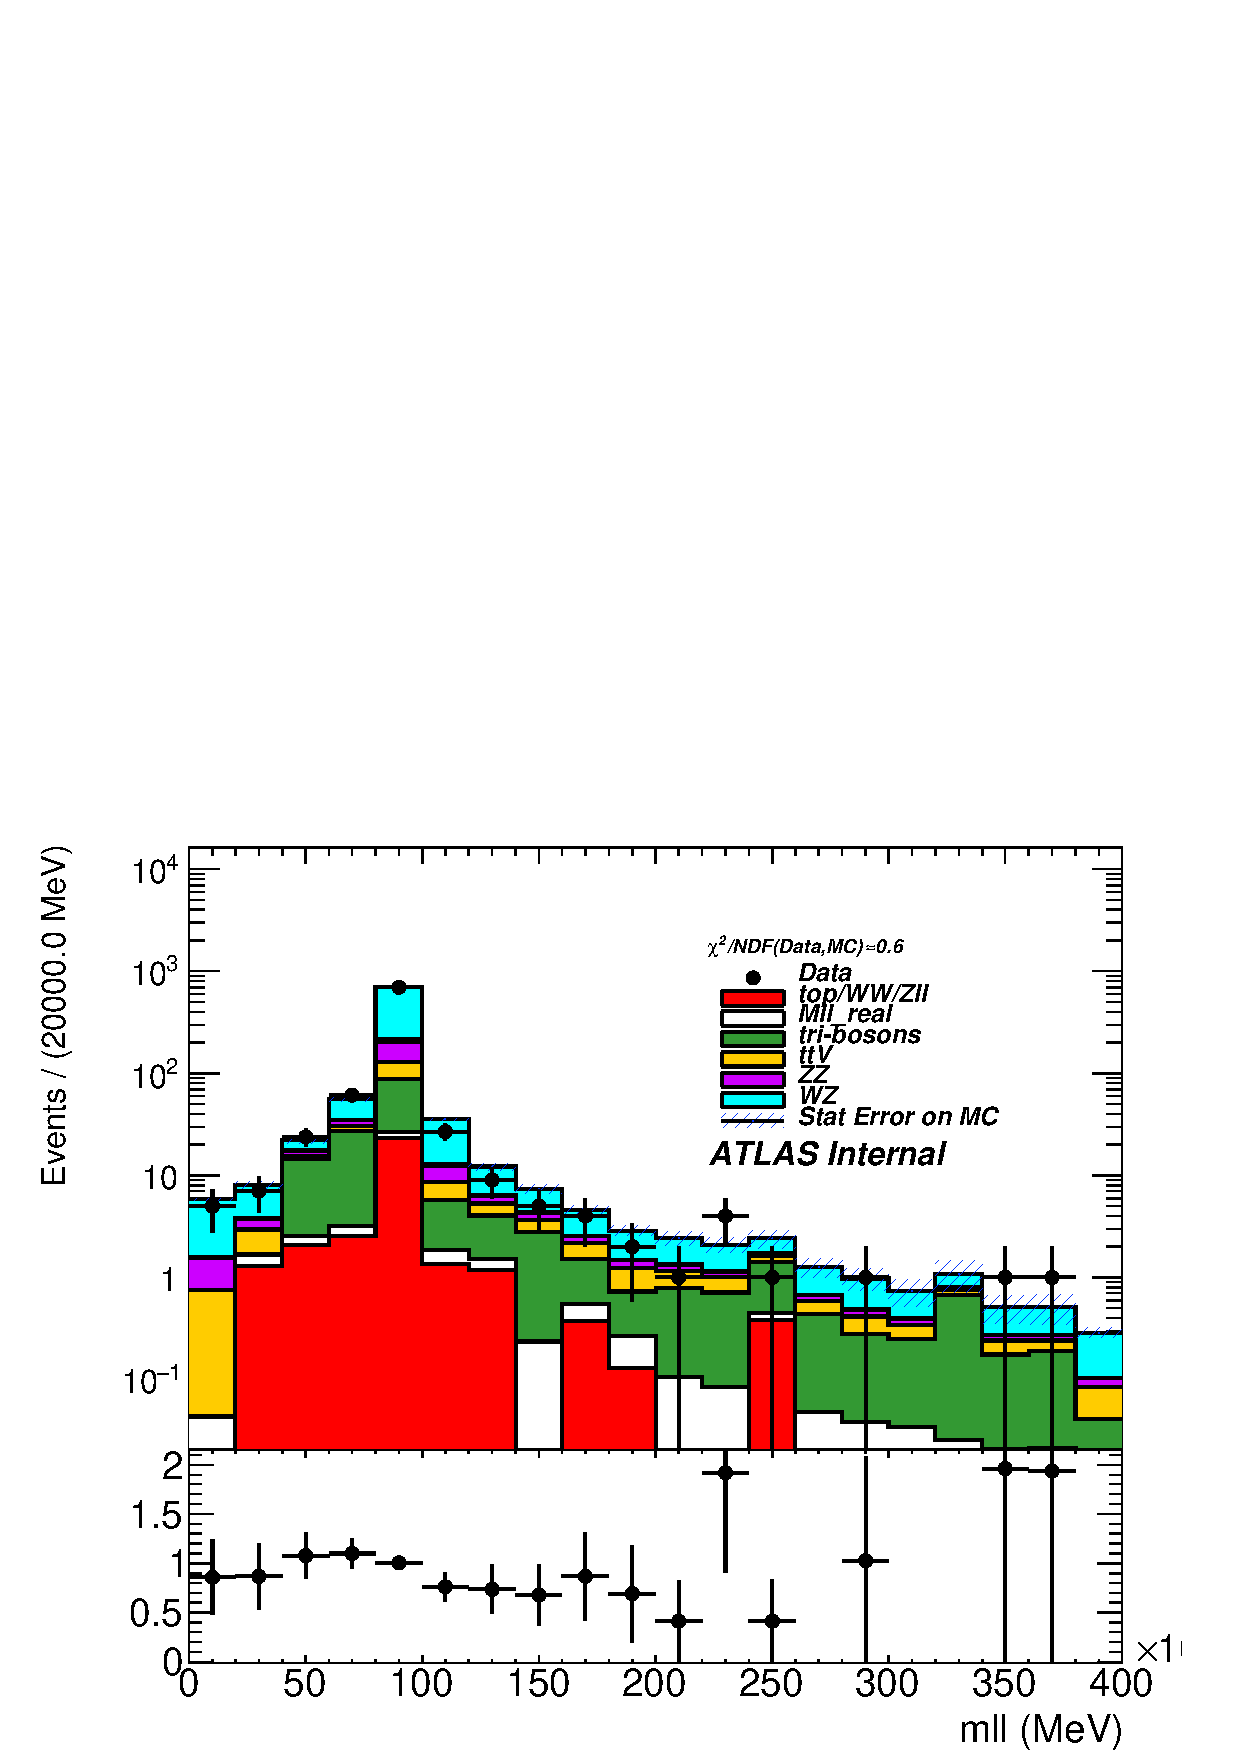
\includegraphics[width=0.45\textwidth]{figures/WZ_CR/2DSideband_WZCR_Isolated}
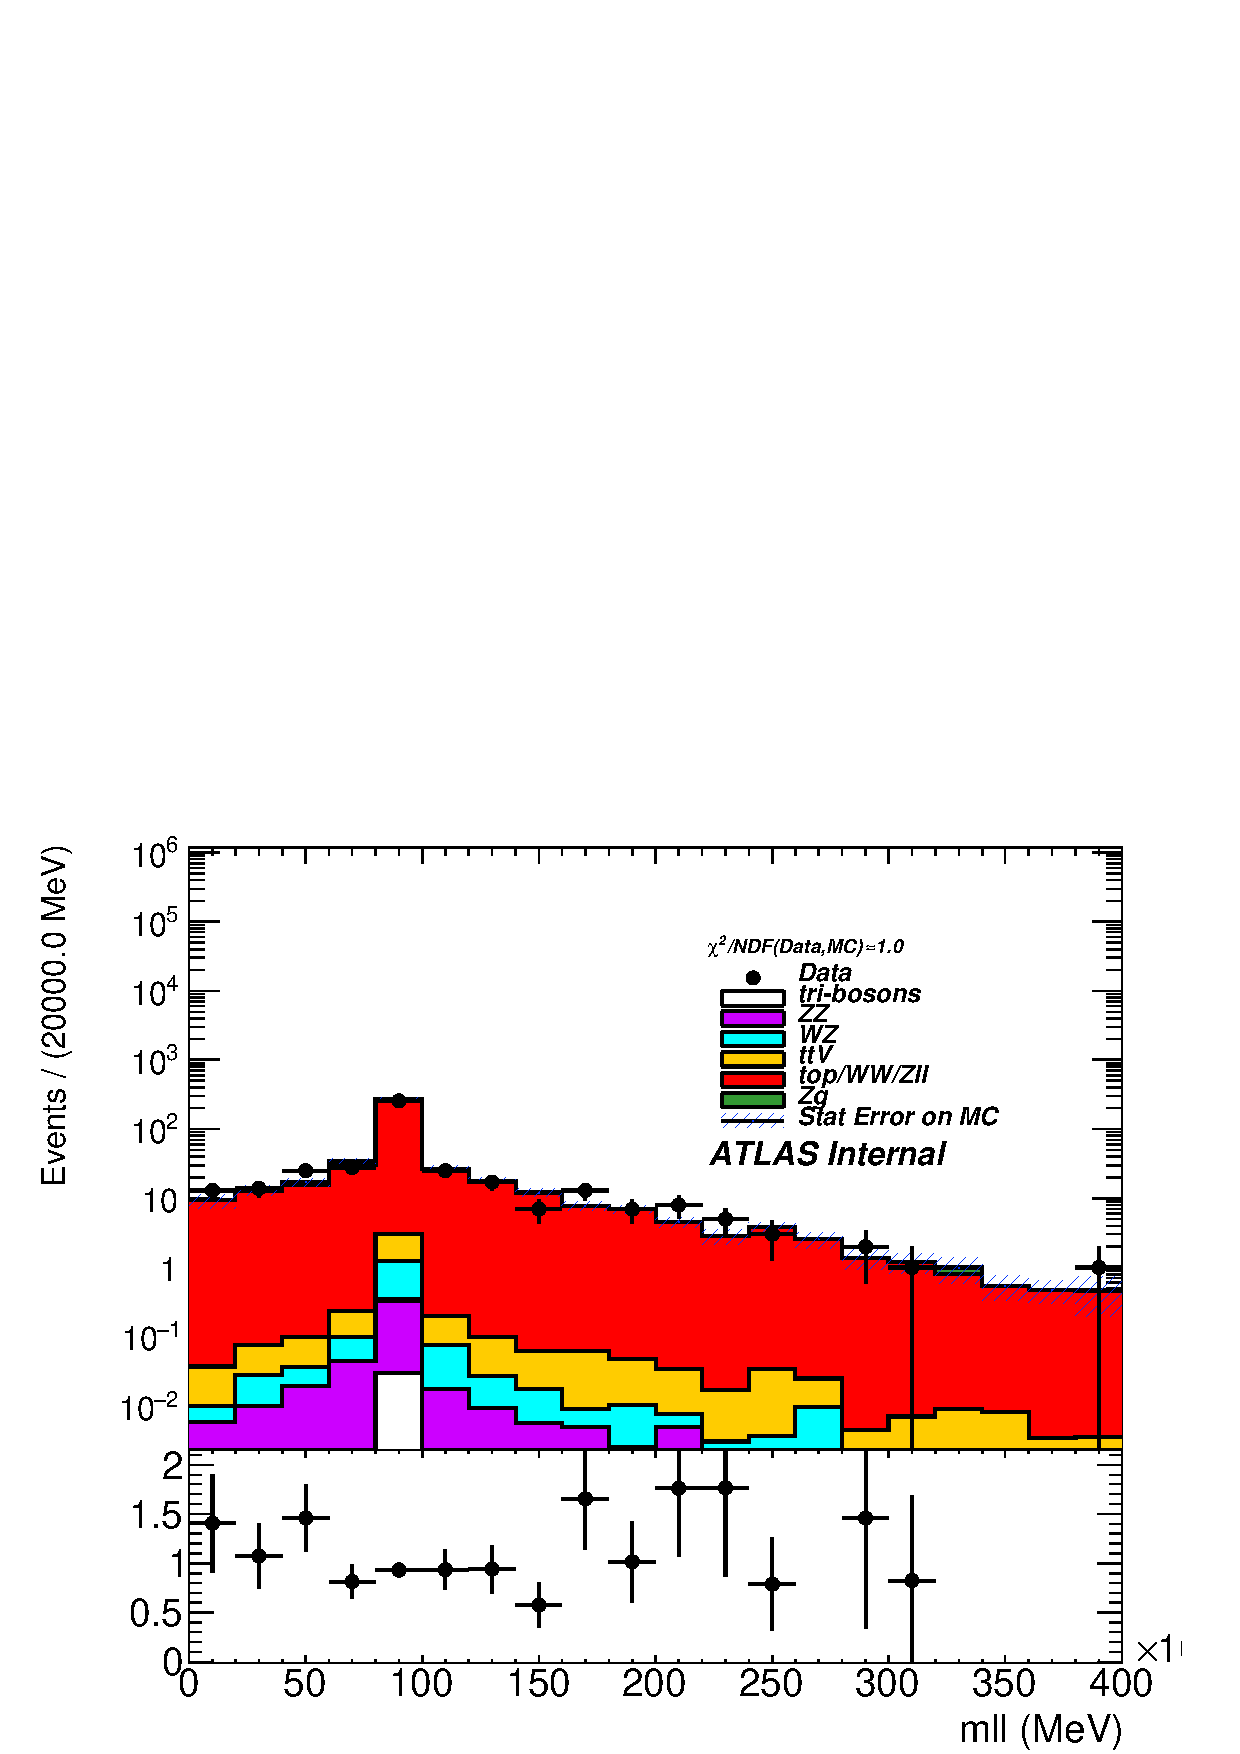
\includegraphics[width=0.45\textwidth]{figures/WZ_CR/2DSideband_WZCR_NonIsolated}
\caption{$WZ$ Control regions. Distribution of the $m_{\ell\ell}^{SFOS}$ in the isolated and anti-isolated CR.}
\label{fig:WZ_CR}
\end{figure}  

\paragraph{Closure test and systematic uncertainties}


To prove that the 2D-sideband method can determine accurately the $WZ$ normalization, MC closure tests are performed. The MC processes of the two isolations regions showed on Figure~\ref{fig:WZ_CR} are summed up. Two templates are obtained, and they are used as if they were data in region A, B, C and D. These templates are used to generate pseudo-datasets which will serve to recompute the number of $WZ$ events with the 2D-sideband method.
Once again the NLO prediction in region A gives $N_A^{WZ}(MC)= 498 \pm 1$, using the pseudo-data one find $N_A^{WZ}(measured)=495.\pm{}39$ events. Other tests are performed: 

\begin{itemize}
\item Scaling up the $WZ$ signal by $20\%$.
\item Scaling up the fake background by $50\%$.
\item Scaling up the EW background by $20\%$.
\end{itemize}

In all these cases the 2D-sideband method allows to retrieve the proper normalization of the $WZ$ signal injected. More information can be found in the Appendix~\ref{appendix:2dsideband}.



Several sources of systematic effects are investigated. The difference between the number of $WZ$ events measured in region A after varying one variable and the central value reported above is taken into account as a systematic. They are listed below, more details can be found in appendix~\ref{appendix:2dsideband}.
\begin{itemize}
\item The isolation cuts are varied to $E_{T}^{Iso(R<0.2)}/E_{T}>0.25$ and $p_{T}^{Iso(R<0.2)}/p_{T}>0.2$, in order to check the impact of this cut on the measured number of events. The total number of $WZ$ events found in this case is: $N_A^{WZ}(measured)=539 \pm 35$, which yield a systematic uncertainty of $0.5\%$ on the normalization factor.

% \item The $p_{T}$ cut on the 3rd lepton is varied by $\pm{}1~\GeV$, the largest deviation found is taken as a systematic on the normalization factor. It is found that the largest difference in the normalization factor is found when varying the lepton $p_{T}$ to $26~\GeV$. In this case the predicted number of events is found to be: $N_A^{WZ}(\mbox{MC})=468{}\pm 1$ while the measured number of events in the data is found to be $N_{\mbox{WZ}}^{\mbox{data}(Ori)} =492 \pm 34$, which yield a ratio of $1.05 \pm 0.07$, or a difference of $2.9\%$ with the nominal normalization factor.
 
\item The cut on the $m_{\ell\ell}$ is increased to $35~\GeV$ in the definition of region B and D. The total number of $WZ$ events found in this case is: $N_A^{WZ}(measured)=557. \pm 35$ , which yield a ratio of $1.12 \pm 0.07$, or a difference of $3.7\%$ with the nominal normalization factor.

\item The normalization of the backgrounds taken from MC, which are subtracted, is varied by $20\%$ up and down and the largest difference is taken as another systematic uncertainty. It is found that the largest uncertainty is obtained by varying up the normalization of these backgrounds. In this case one find $N_A^{WZ}(measured)=558 \pm 35$, which gives a ratio of $1.12 \pm 0.07$, or an uncertainty of $3.8\%$ compared to the central prediction.

 
\item Finally the $R^{jet}$ factor is varied from $R^{jet} =1.$ to the value measured in MC: $R^{jet} =0.61 \pm 0.24$. The uncertainty on this factor is quite large due to the very low statistics available in MC in the isolated control regions. $N_A^{WZ}(measured)=527. \pm 136.$, which gives a correction factor of $1.06 \pm 0.23$. This yield a systematic uncertainty of $2.4\%$ on the normalization factor.

\end{itemize}

All these uncertainties are added in quadrature giving a total systematic uncertainty of $5.9\%$ on the scale factor. The final correction factor on the normalization of the $WZ$ background is therefore: $k_{WZ}=1.08 \pm 0.07^{stat} \pm 0.07^{sys}$.

\paragraph{Validation}

In order to check the consistency of the scale factor determined above, the agreement between the data and the model is checked in a region passing the event pre-Selection cuts and containing exactly two SFOS lepton pairs. Figure~\ref{fig:WZ_2SFOS_CR} show the leading lepton \pt{}, the \MET{}, the invariant mass distribution of the two leading lepton \pt{}, and the jet multiplicity in this region. Table~\ref{tab:presel_2sfos_wzval} show the overall yields predicted by the model and observed on the data. The data agrees very well with the model in this region after using the k-factor presented above.

\begin{table}[ht!]
\centering
\begin{tabular}{|c||c|c|c|c|}
\hline
 & $eee$ & $ee\mu$ & $e\mu\mu$ & $\mu\mu\mu$\\ 
\hline\hline
$WZ$ &  $240.28 \pm 0.67$(stat) $\pm 21$(syst) &  $0.0 \pm 0$ &  $0.0 \pm 0$ &  $567.0 \pm 1$ $\pm 50$(syst)\\ 
$ZZ$ &  $60.07 \pm 0.13$ &  $0.0 \pm 0$ &  $0.0 \pm 0$ &  $91.48 \pm 0.17$\\ 
$Z\gamma$ &  $69.9 \pm 2.7$ &  $0.0 \pm 0$ &  $0.0 \pm 0$ &  $0.17 \pm 0.12$\\ 
$ZWW+ZZZ$ &  $0.435 \pm 0.019$ &  $0.0 \pm 0$ &  $0.0 \pm 0$ &  $0.864 \pm 0.028$\\ 
$t\bar{t}+V$ &  $4.845 \pm 0.044$ &  $0.0 \pm 0$ &  $0.0 \pm 0$ &  $10.509 \pm 0.066$\\ 
Fake (data-driven) &  $44.9 \pm 2.2$ &  $0.0 \pm 0$ &  $0.0 \pm 0$ &  $42.4 \pm 1.2$\\ 
$WWW$ &  $0.768 \pm 0.011$ &  $0.0 \pm 0$ &  $0.0 \pm 0$ &  $1.843 \pm 0.018$\\ 
\hline
Expected Background &  $420.4 \pm 3.5$ $\pm 21$(syst)&  $0.0 \pm 0$ &  $0.0 \pm 0$ &  $712.5 \pm 1.6$ $\pm 50$(syst)\\ 
Expected Signal + Background &  $421.2 \pm 3.5$ $\pm 21$(syst)&  $0.0 \pm 0$ &  $0.0 \pm 0$ &  $714.3 \pm 1.6$ $\pm 50$(syst)\\ 
\hline
Observed Data &  $425 \pm 21$ &  $0.0 \pm 0$ &  $0.0 \pm 0$ &  $757 \pm 28$\\ 
\hline
\end{tabular}

\caption{Expected and observed event yields binned by lepton flavor combination for the following selection: event pre-selection + 2 SFOS. Only the systematic uncertainties on the $WZ$ background due to the k-factor is given. The other uncertainties are only statistical.}
\label{tab:presel_2sfos_wzval}
\end{table}


\begin{figure}[htp]
\centering
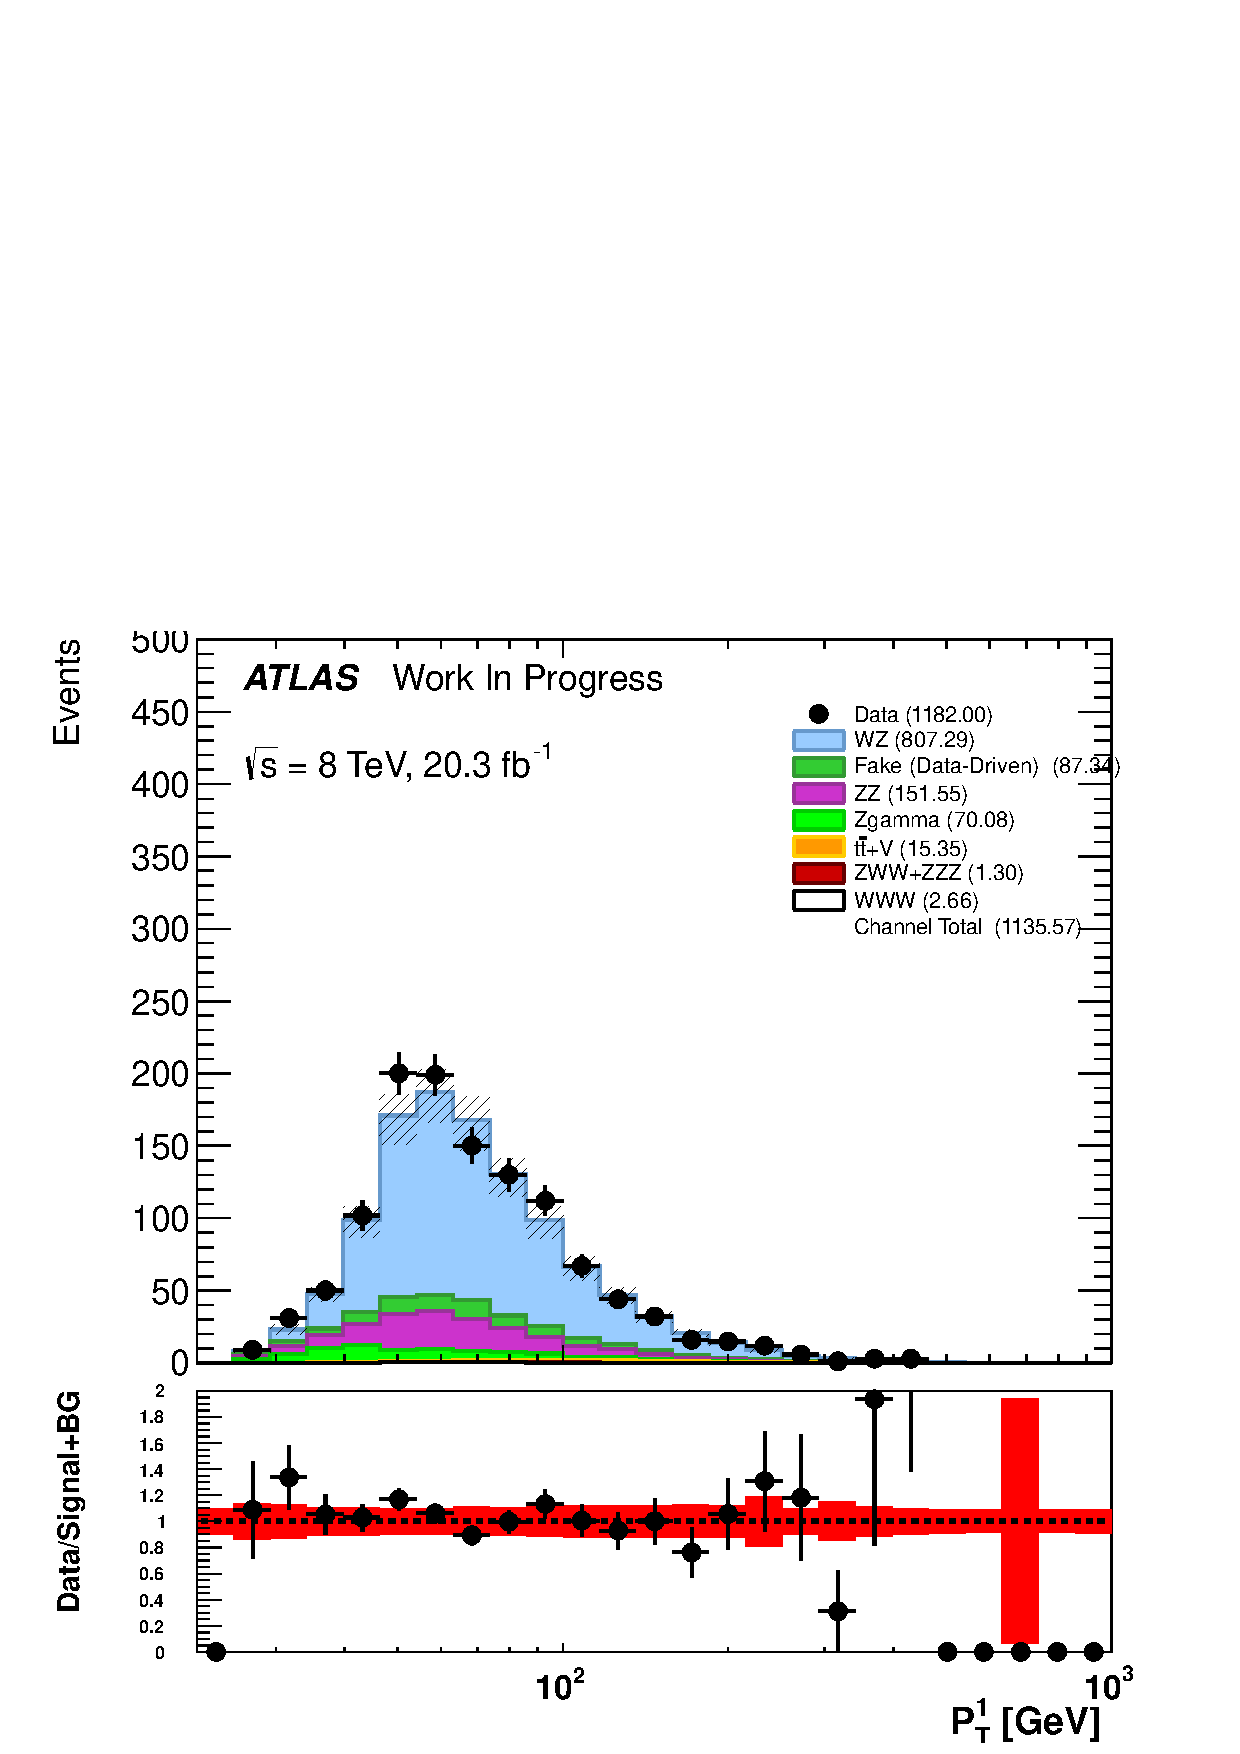
\includegraphics[width=0.4\textwidth]{figures/WZ_CR/LeadingLeptonPt_histratio.png}
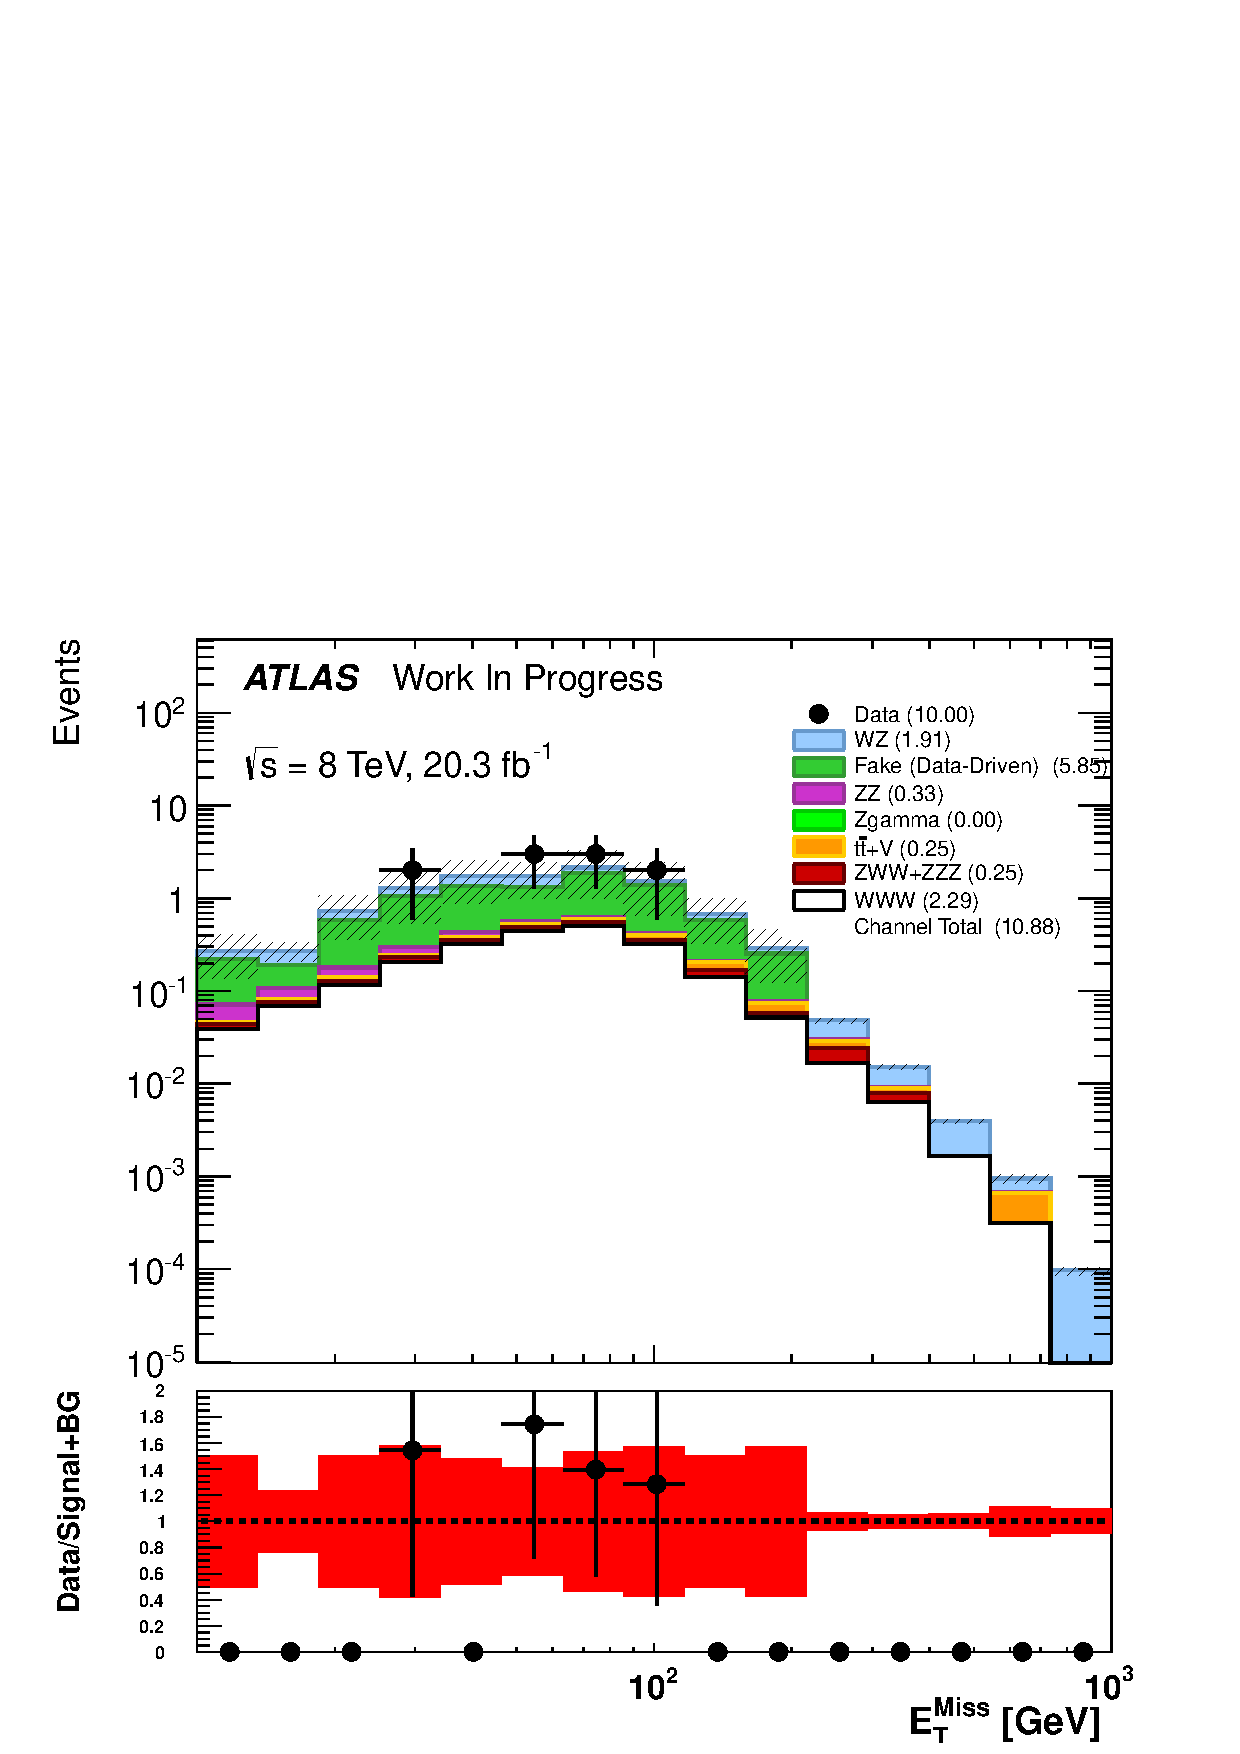
\includegraphics[width=0.4\textwidth]{figures/WZ_CR/MET_Et_histratio.png}
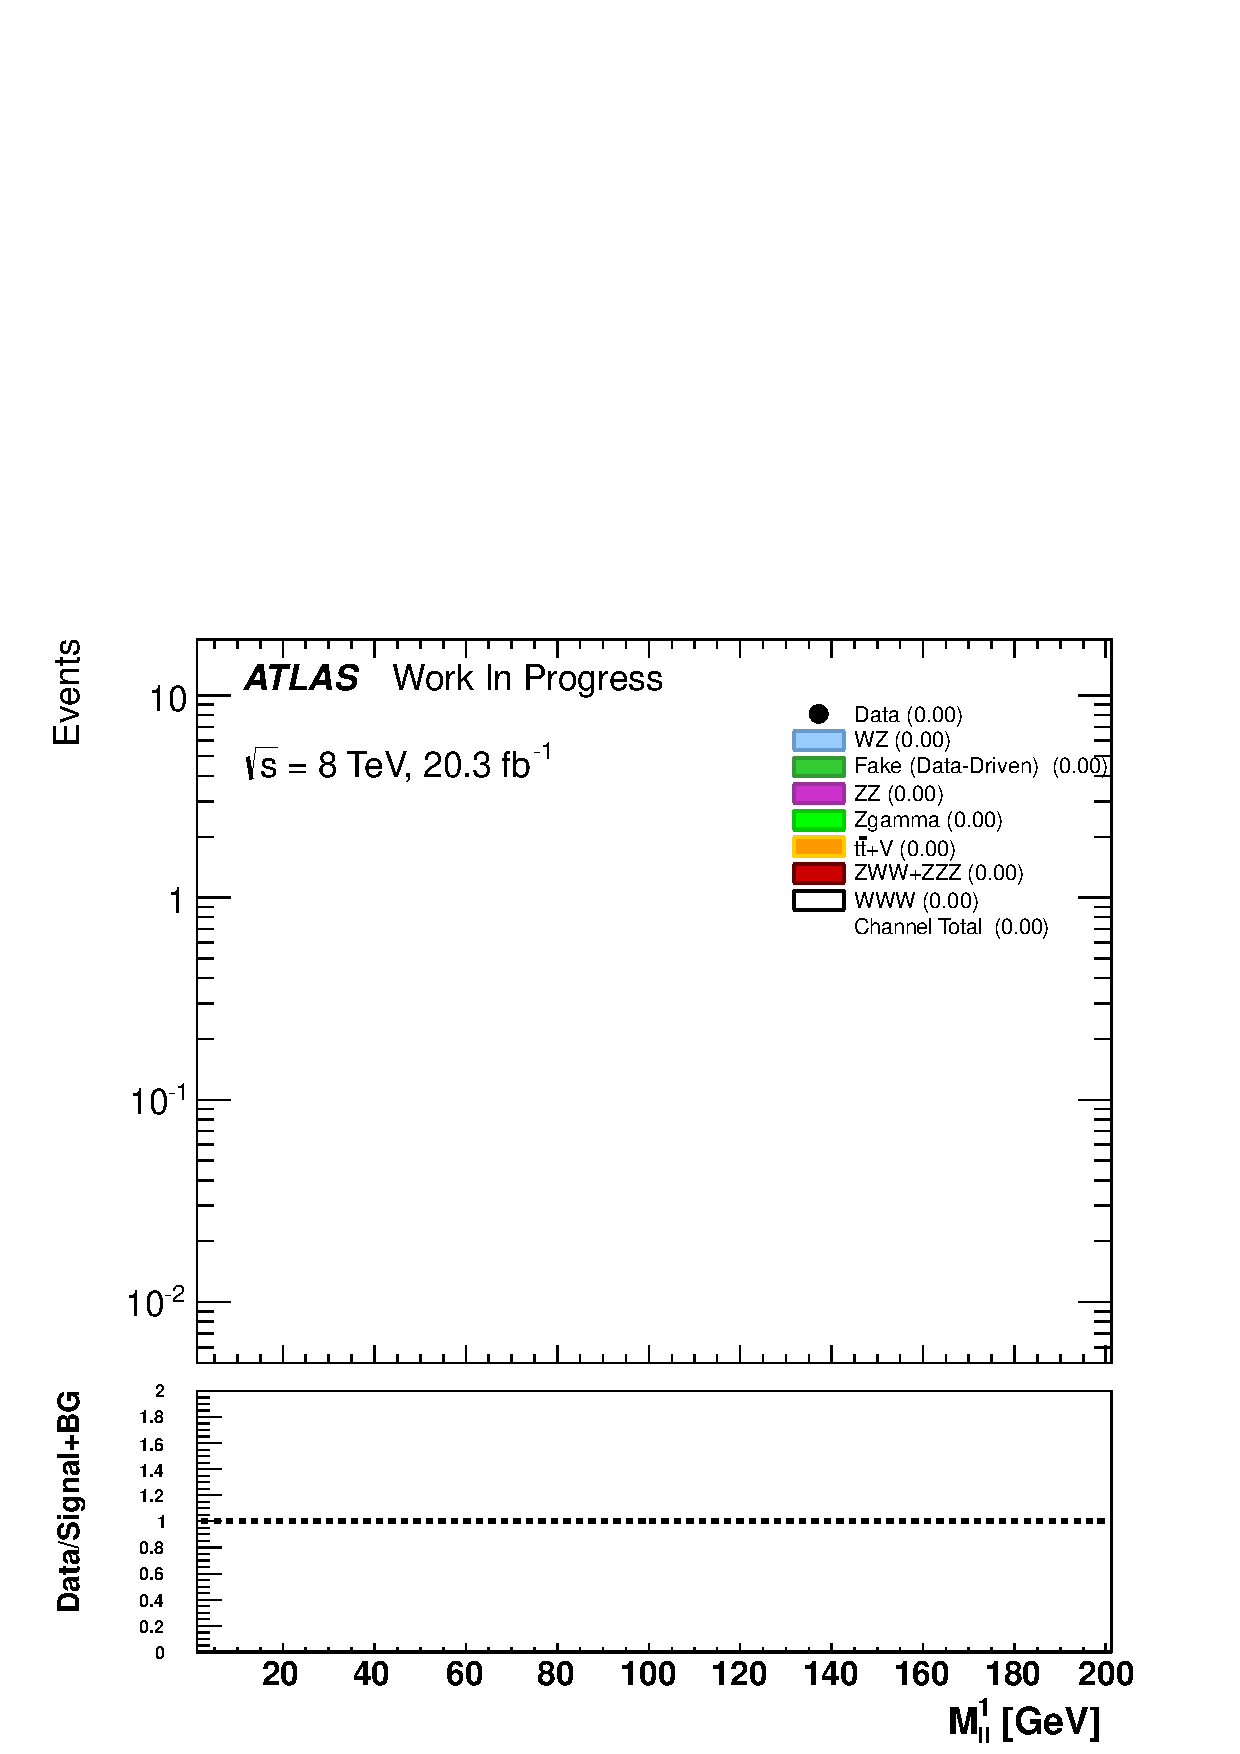
\includegraphics[width=0.4\textwidth]{figures/WZ_CR/InvariantMassSFOS_histratio.png}
\includegraphics[width=0.4\textwidth]{figures/WZ_CR/NJets_histratio.png}

\caption{$WZ$ 2SFOS Control regions. Distribution of leading lepton $p_{T}$, $\MET$, $m_{12}$, and jet multiplicity. The systematic band shows the uncertainty on the WZ k-factor.}
\label{fig:WZ_2SFOS_CR}
\end{figure}  


\clearpage

\subsubsection{$ZZ$}
\label{sec:zzbg}

Another important process that participate to the 3 lepton final state, is due to the $ZZ^{*}$ production, where one lepton goes out of the detector acceptance, or doen't pass the selection criteria. The $ZZ^{*}$ backgrounds are modelled using the Powheg generator, and the $gg2ZZ$ generator for the loop induced processes. The normalization of the non-loop induced processes are scaled up to NNLO predictions using a kfactor which is 1.05, as defined in~\cite{Cascioli:2014yka,Baglio:2013toa,Bierweiler:2013dja}. The total systematic uncertainty associated to the theoretical predictions in this final state is taken to be $15\%$~\cite{Cascioli:2014yka,Baglio:2013toa,Bierweiler:2013dja}.

The agreement between data and the model is then checked in a control region, where 2 same flavors opposite sign pairs leptons ($e$ and $\mu$) are requested. The leptons must follow the quality requirements defined in Section~\ref{sec:Object_selection}. The transverse momentum of the leptons should be: $p_{T}^{1}>25~\GeV$, $p_{T}^{2}>15~\GeV$, $p_{T}^{3}>15~\GeV$, and  $p_{T}^{4}>10~\GeV$. The pairing of the leptons follows the algorithm defined in~\cite{Aad:2014wra}. In order to remove any contribution from fake backgrounds, only the events where the two $Z$ bosons are on shell are kept, \textit{ie}: $60<m_{12}<120~\GeV$ and $60<m_{34}<120~\GeV$. Figure~\ref{fig:ZZ_CR}, show the distributions of $m_{12}$, $m_{34}$, $m_{4l}$, and the leptons $p_{T}$ for this selection, while Table~\ref{tab:ZZ_CR} gives the total number of event measured in this CR and the prediction on the different processes in the same region.

The agreement between the data and the MC predictions is very good, for the shape or for the prediction of the total number of events in this control region.

It was also checked whether or not the contribution of $ZZ^{*}$ where the $Z^{*}$ boson is very offshell, $m_{Z^{*}} < 4$~GeV, while the other boson
has a  mass $m_Z > 4$~GeV has any impact on the signal regions. This was evaluted by looking at the samples with channel numbers
$181471$ through $181479$ in Table~\ref{tab:sample_bkg_dibosons}.  The contribution from these samples were found to be negligible, with a statistical
uncertainty compatible with exaxtly 0 events in the individual signal regions. As a result, these samples were not considered any further and are not
included in the final background  estimate for the signal regions or in the ZZ control regions.


\begin{figure}[htp]
\centering
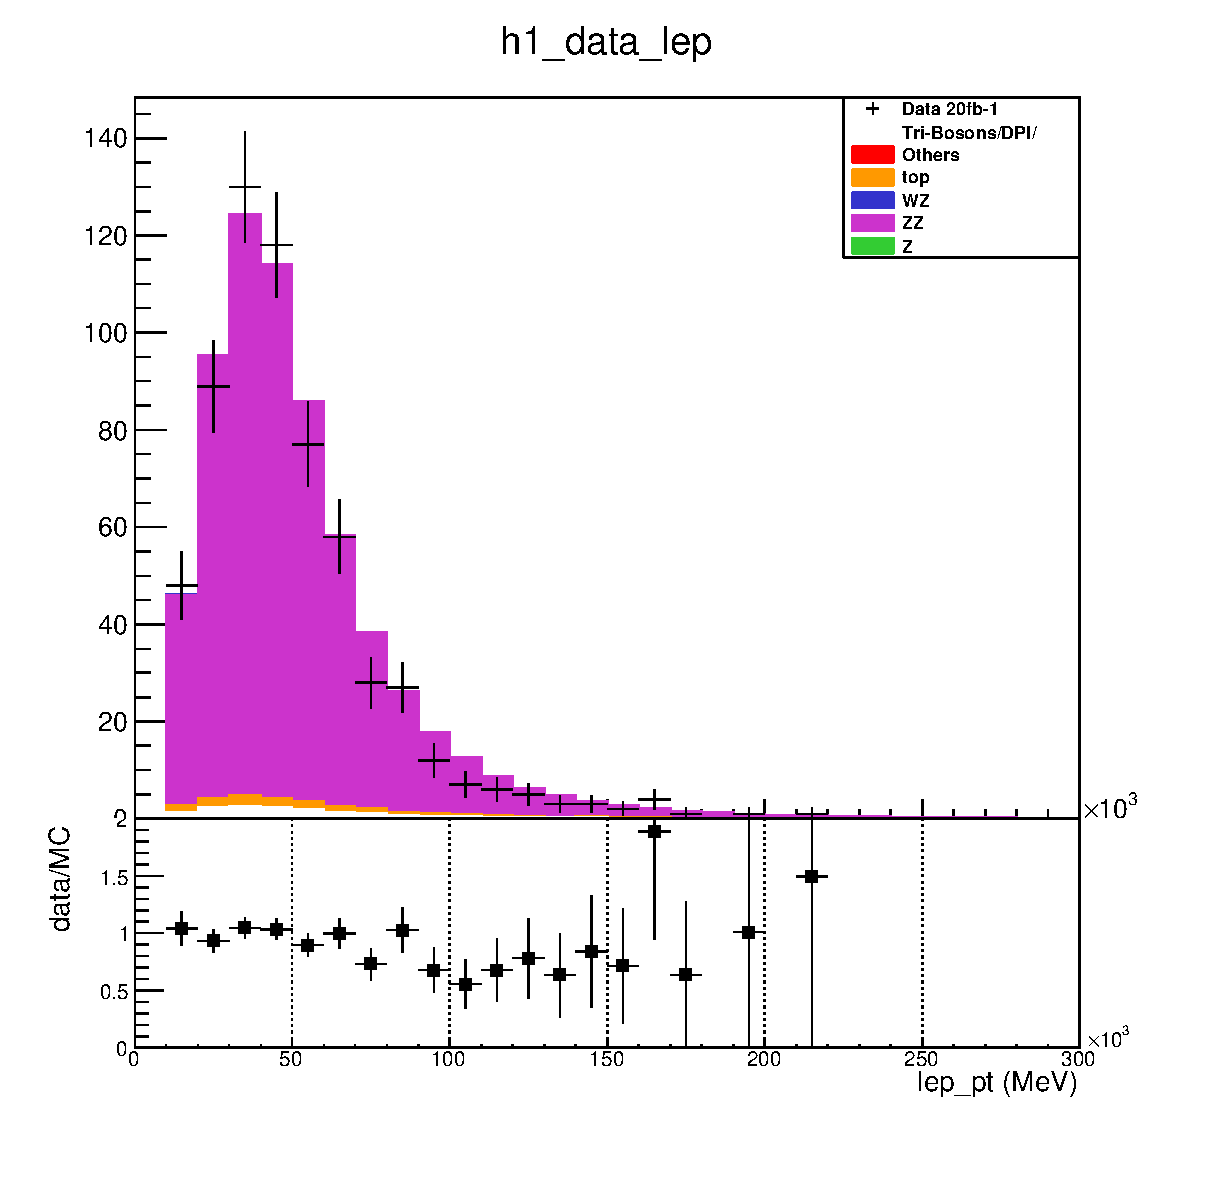
\includegraphics[width=0.4\textwidth]{figures/ZZ_CR/ZZ_CR_lep_pt.eps}
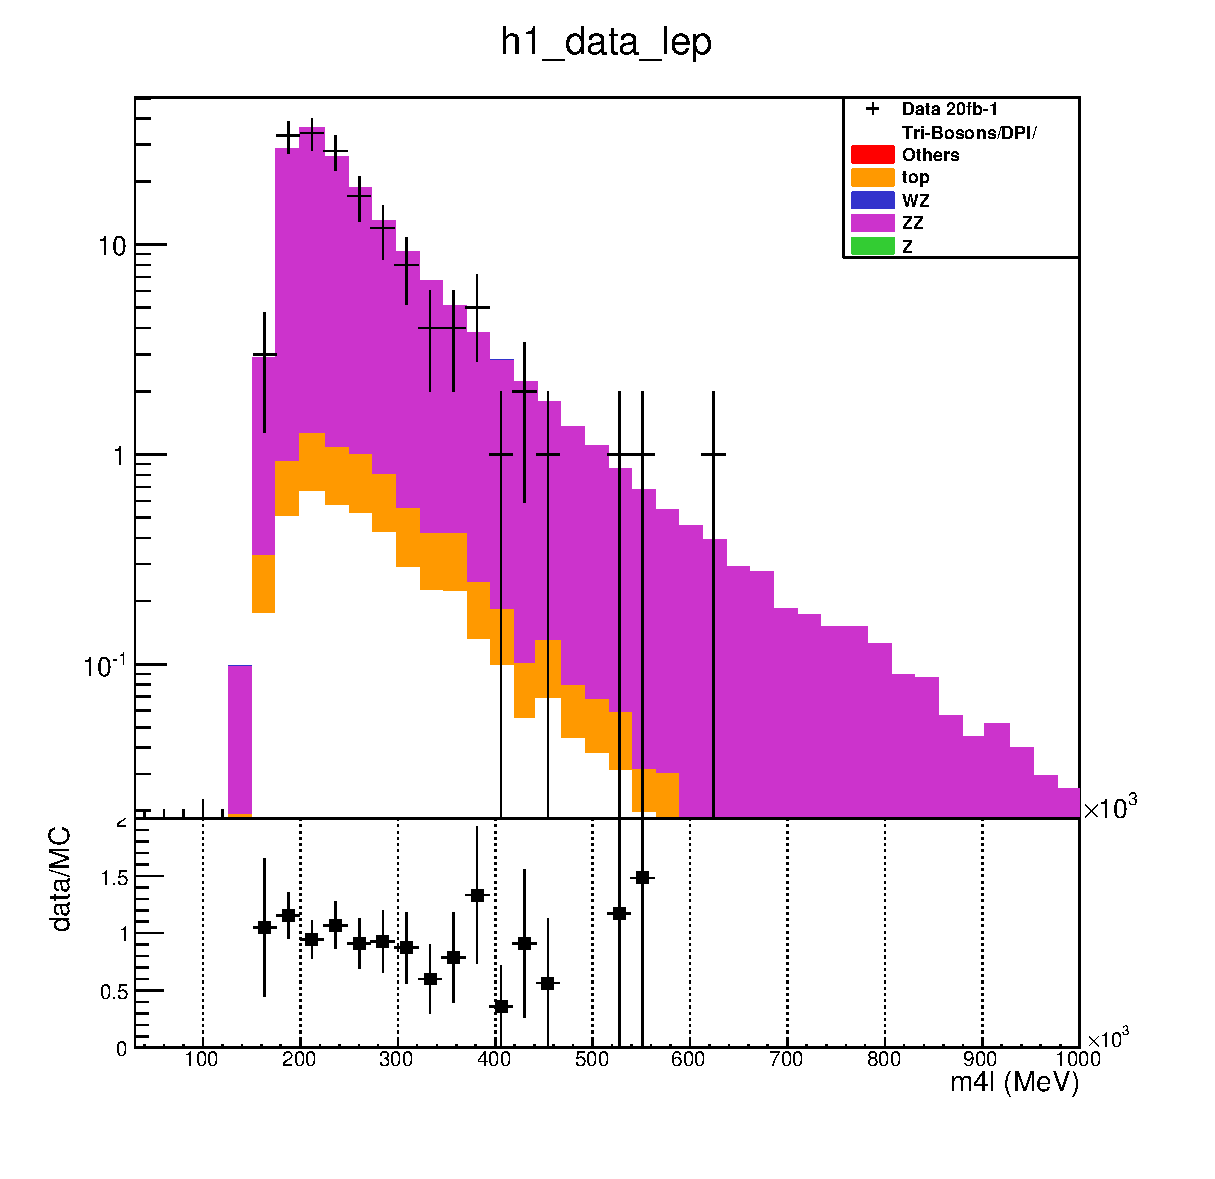
\includegraphics[width=0.4\textwidth]{figures/ZZ_CR/ZZ_CR_m4l.eps}
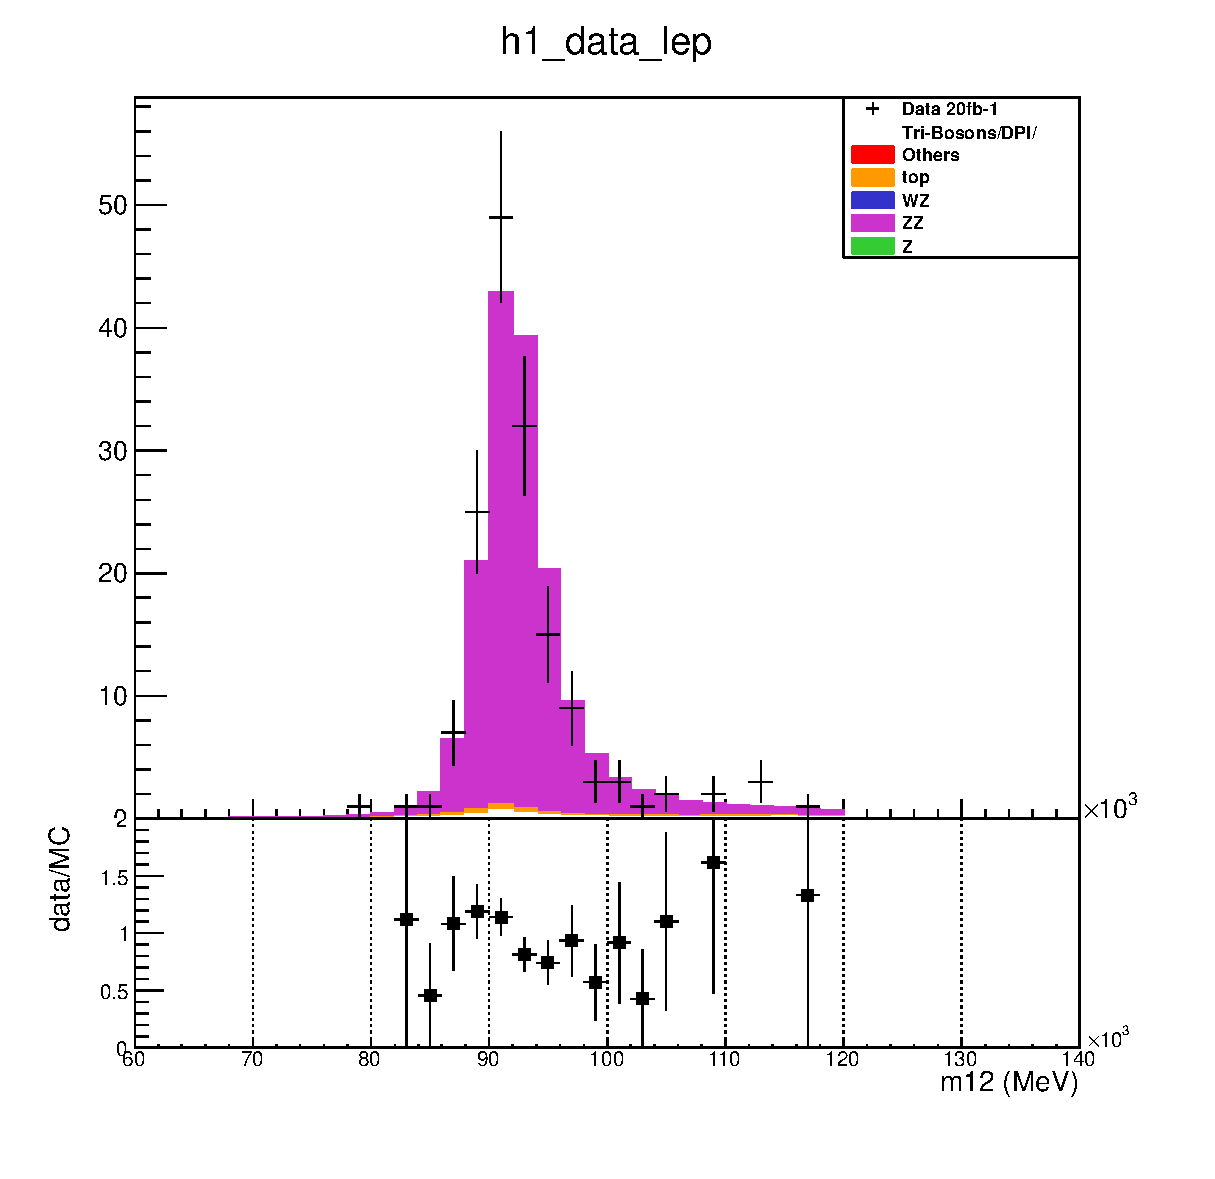
\includegraphics[width=0.4\textwidth]{figures/ZZ_CR/ZZ_CR_m12.eps}
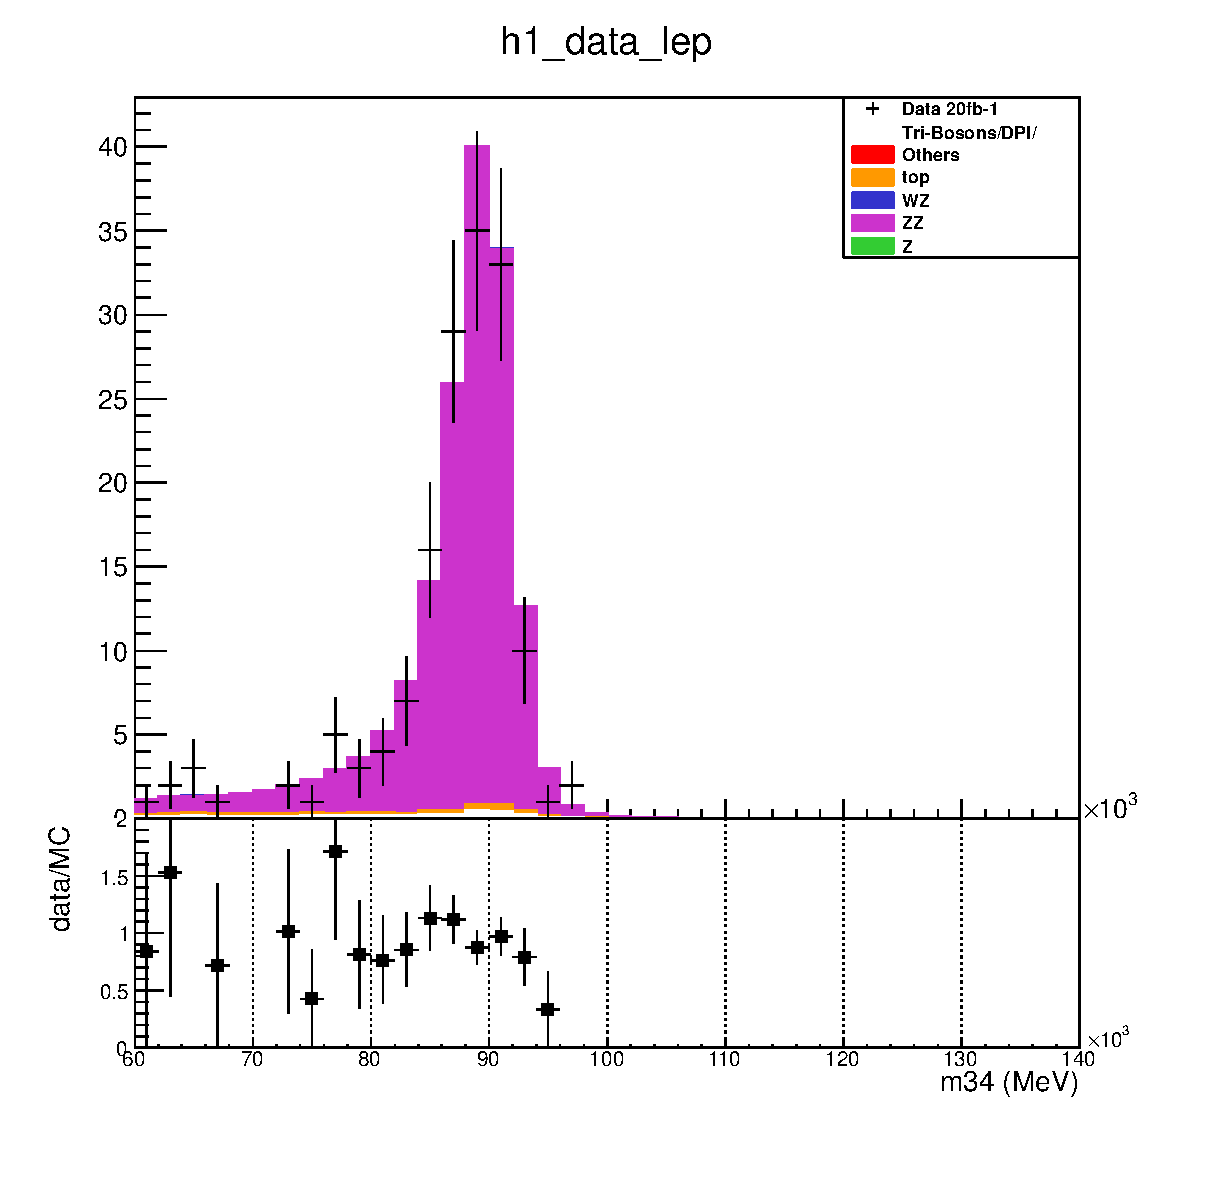
\includegraphics[width=0.4\textwidth]{figures/ZZ_CR/ZZ_CR_m34.eps}

\caption{$ZZ\to{}4\ell$ Control regions. Distribution of leptons $p_{T}$, $m_{12}$, $m_{34}$, $m_{4l}$.}
\label{fig:ZZ_CR}
\end{figure}  

\begin{table}[htp]
\centering
\begin{tabular}{|c||c|c|c|c|}
\hline
 & Event Yield\\ 
\hline\hline
$WZ$ &  $0.05 \pm 0.01$\\ 
$ZZ$ &  $156.2 \pm 0.3$(stat) $\pm 22.3$(syst) \\ 
% $gg2ZZ$ &	$21.3 \pm 0.2$ \\
$Z\gamma$ &  $0.0 \pm 0.0$\\ 
Fake (MC) &  $3.6 \pm 0.2$\\ 
triboson and $t\bar{t}+V$ &  $4.1 \pm 0.2$\\ 
\hline
Expected Signal + Background &  $164.0 \pm 0.3$ (stat) $\pm 22.3$(syst)\\ 
\hline
Observed Data &  $155 \pm 12$\\ 
\hline
\end{tabular}
\caption{Number of data and predicted events in the ZZ CR. The error quoted on the MC samples represents only the statistical error on the MC samples. The systematic error due to theoretical normalization on the $ZZ$ sample is also showed.}
\label{tab:ZZ_CR}
\end{table}


\clearpage

\subsubsection{$Z\gamma$}

The $Z\gamma$ process, where the $Z$ boson decays to a pair of leptons ($e$ and $\mu$), is estimated from MC. This proces is obtained using the Sherpa generator. It was found that Sherpa describes accurately the shape and normalization of data in the $7~\TeV$ and $8~\TeV$ datasets~\cite{Aad:2013izg,Auerbach:1631102}. Therefore the normalization of these sample is taken to be the cross-section provided by the Sherpa generator. These processes are contributing to our selection, via the conversion of one photon into a pair of electrons, and then the loss of one of these electrons in the acceptance. 

These effects are expected to be properly described by the simulation, but the agreement between the data and the model is checked in a control region where the events are requested to contains exactly two muons and one electron, and the tri-body invariant mass of this system, should be close to the $Z$-pole mass~\cite{PDG:2014}: $|m_{\mu\mu{}e}-91.19|<15~\GeV$.

Figure~\ref{fig:Zgamma_CR} shows the invariant mass distribution of the 3 leptons, the leptons $p_{T}$, the $\eta$ distribution of the electron, and the jet multiplicity. The normalization in the CR is also checked and is provided in Table~\ref{tab:Zgamma_CR}.
All the distributions and the event yield show a very good agreement between the data and the model.

\begin{figure}[htp]
\centering
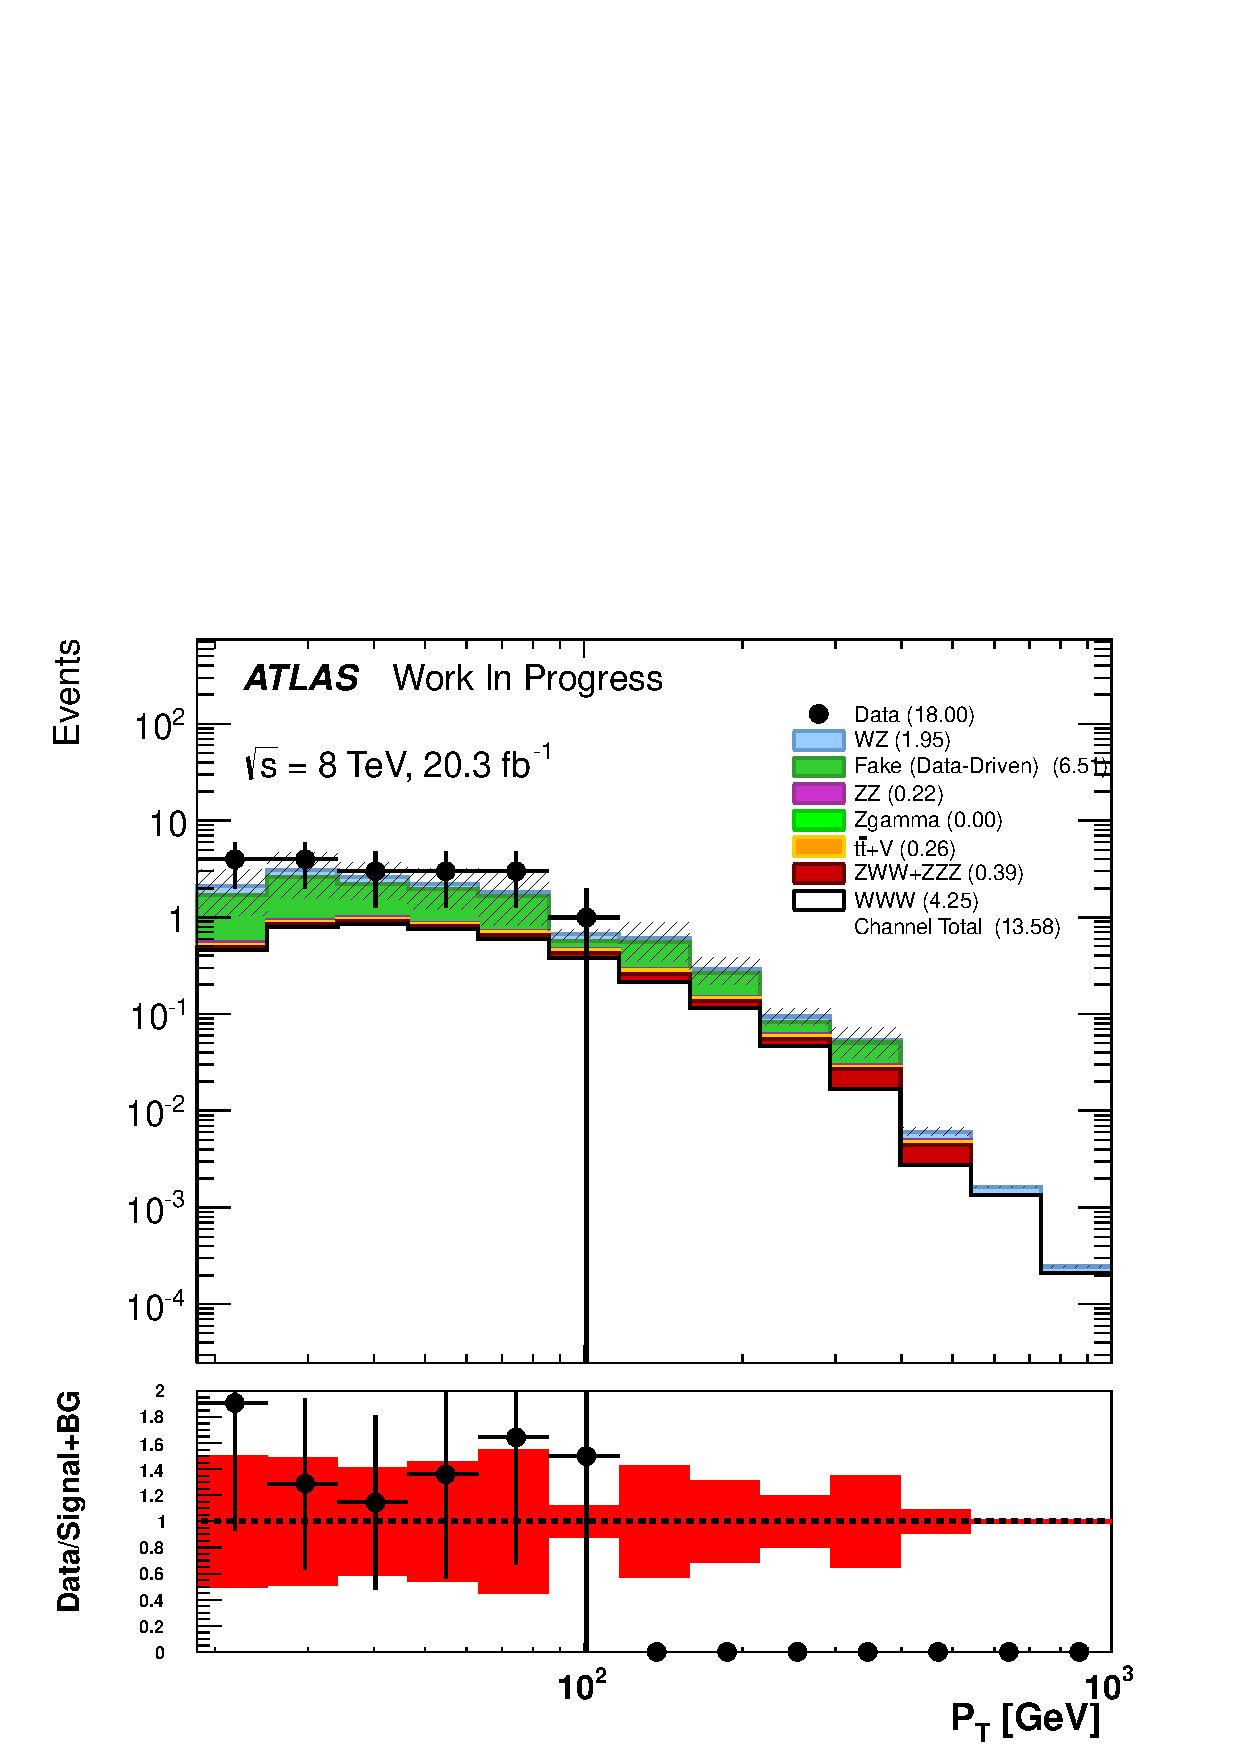
\includegraphics[width=0.4\textwidth]{figures/ZG_CR/AllLeptonPt_histratio.png}
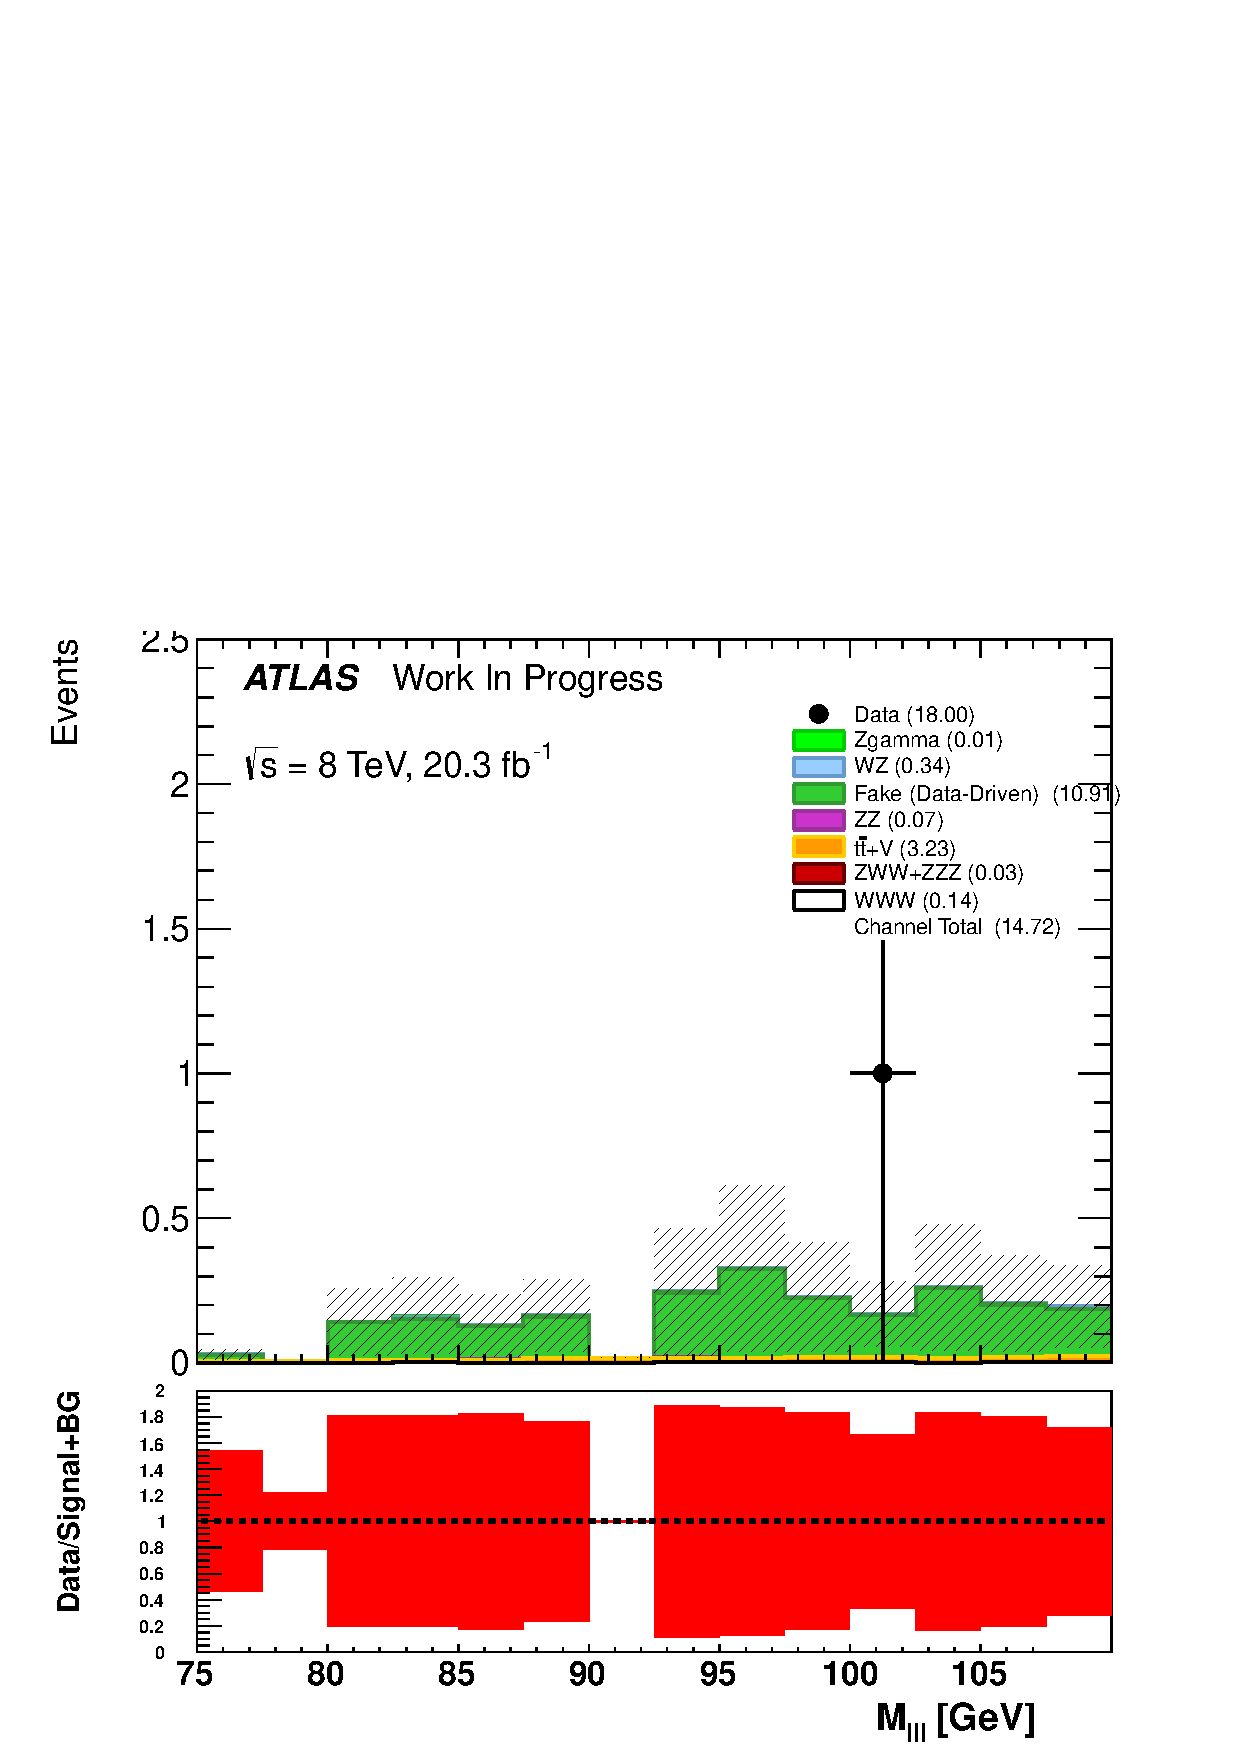
\includegraphics[width=0.4\textwidth]{figures/ZG_CR/InvariantMassThreeLep_histratio.png}
\includegraphics[width=0.4\textwidth]{figures/ZG_CR/ElectronEta_histratio.png}
\includegraphics[width=0.4\textwidth]{figures/ZG_CR/NJets_histratio.png}

\caption{$Z\gamma$ Control region. Distribution of leptons $p_{T}$, invariant mass of the 3leptons, electron $\eta$, and jet multiplicity.}
\label{fig:Zgamma_CR}
\end{figure}  


\begin{table}[ht!]
\centering
\begin{tabular}{|c||c|c|c|c|}
\hline
 & Event Yield\\ 
\hline\hline
$WZ$ &  $7.47 \pm 0.11$\\ 
$ZZ$ &  $9.116 \pm 0.075$\\ 
$Z\gamma$ &  $80.3 \pm 2.8$\\ 
$ZWW+ZZZ$ &  $0.0285 \pm 0.0046$\\ 
$t\bar{t}+V$ &  $0.338 \pm 0.012$\\ 
Fake (data-driven) &  $21.9 \pm 1.2$\\ 
$WWW$ &  $0.3142 \pm 0.0072$\\ 
\hline
Expected Background &  $119.2 \pm 3.1$\\ 
Expected Signal + Background &  $119.5 \pm 3.1$\\ 
\hline
Observed Data &  $119$\\ 
\hline
\end{tabular}

\caption{Expected and observed event yields for the Z$\gamma$ control region. Only the statistical uncertainties are showed.}
\label{tab:Zgamma_CR}
\end{table}



\subsubsection{Double parton scattering, $\ttbar + V$, and $VVV$}

\paragraph{DPS}
\label{sec:bkg_DPS}
Double parton scattering (DPS) backgrounds are also taken into account in the analysis. To estimate their contribution a list of samples used in the same sign WW analysis~\cite{Aad:2014zda,DPS:Twiki} has been used. The cross section of these processes can not be taken directly from MC, but it must be further studied. Considering the DPS production of $A+B$, where $A$ and $B$ can be products of any single-parton, the cross section can can be factorised as~\cite{Gaunt:2010pi}:
\begin{equation}
	\sigma^{DPS}_{(A+B)}=\frac{m}{2}\times{}\frac{\sigma^{S}_{A}\times{}\sigma^{S}_{B}}{\sigma_{eff}}
\end{equation}	

Where $\sigma^{S}_{(A/B)}$ is the single-parton scattering production cross-section of the process $A/B$, $m$ is a factor which takes the value of 1 when $A=B$ and 2 when $A\ne B$, $\sigma_{eff}$ is the effective cross section of the proton. A measurement of $\sigma_{eff} =15\pm3(stat)^{+5}_{-3}(syst)$ mb for 7~\TeV{} $p-p$ collisions has been recently performed by ATLAS~\cite{Aad:2013bjm}. By factorizing the cross-section in this form, the correlation between the two parton interactions are neglected.

The samples and cross section that have been used in this analysis are given in Table~\ref{tab:sample_bkg_dibosons_gg2DPI}. An uncertainty of $50\%$ is applied on the normalization of these processes. Among these processes the one that can give a tri-lepton final state are: $WZ$, $ZZ$, and $Z\gamma$.
	
Their contributions are found to be negligible.


\paragraph{Other backgrounds}
The other backgrounds evaluated from MC are the one containing three real leptons: $t\bar{t}+V$, $WWZ$, and $WZZ$.
The PDF and scale uncertainties for the $t\bar{t}+V$ processes have been evaluated by other member of the ATLAS collaboration~\cite{ttV:Twiki}, and found
to be about $30\%$ of their normalization. These processes have been recently measured by the ATLAS collaboration~\cite{ATLAS-CONF-2015-032}, and their normalization are found to be consistent with the NLO predictions.

An equivalent $30\%$ uncertainty is assigned for the other $VVV$ contributions ($ZWW^{*}$ and $ZZZ^{*}$) that are not coming from our signal.

% Other background contributions are arising from tt¯+V, t+V and VVV processes. They will be estimated
%  using MC samples and global normalization uncertainties are associated to these MC predictions. An
%  uncertainty of 30\% is assigned to the tt¯+ V contribution, according to [27]. An uncertainty of 30\% is
%  also assigned to the VVV contribution.

\subsection{Electron Charge Mis-identification}
\label{sec:charge_misid}

%include diagram

High energy electrons\footnote{Throughout this section we use 
electrons to collectively refer to both electrons and positrons
unless otherwise specified.} produced from the 
hard scatter of the proton-proton
collisions of the LHC
will frequently radiate photons in the presence of the ATLAS
detector material. Furthermore, it is also common %how common?
for high energy photons to decay into an electron-positron pair.
These two processes are shown as Feynman diagrams 
separately in \fig\ref{}.
Chaining these two processes together will cause 
an electron (positron) to radiate a photon which then produces an
electron-positron pair, resulting in a three body final state with
two electrons (positrons) and a positron (electron).
Often, the energy difference between the products in the final state will
be large, such that the most of the energy is carried away in only one
product.  It is thus possible that majority of the energy of the initial
electron (positron) is carried away in the positron (electron), which
has an opposite charge.  If the energy imbalance is large enough,
the other two final state electrons (positrons) may not have enough
energy to be reconstructed. As a result, the initial electron
(positron) will instead be measured as a positron (electron), and the 
charge of initial state electron (positron) will have effectively 
been mis-identified. 


%need to do some research on bethe-bloche.
The probability of this to occur is non-negligible in the presence of the material 
from the ATLAS detector. This is due to bremstraahlung...
Look in 'experimental foundations' and in 'particle detection'


While muons are also technically also capable of such a phenomenon, the 
energies required are too large, according to bethe-bloche.
Indeed, we observe that the rate of charge mis-identification for muons
is vanishingly small and so we neglect it. %or should I just say that it should be?

The strong dependence upon the ATLAS material means that care must be
taken when describing this process. In particular, the material 
description in MC, while sophisticated, is not perfect. Thus, the use of MC
for determining the rate of electron charge mis-identification is inherently
flawed. Instead, it would be better to use the data itself to determine
a model for these rates. 
Thus, we extract the rates of electron charge 
mis-identificatoin using the data and only use the rates determined
in MC as a cross-check.

The background due to electron charge mis-identification is most important 
for this analysis
in the 0 SFOS signal region, described in \sec\ref{sec:signal_regions},
where it is one of the only mechanisms by which the $WZ$ and $ZZ$ 
processes enter this region\footnote{The $WZ$ and $ZZ$ processes
can also enter in the 0 SFOS region if the $Z$ bosons
decay to $\tau$ leptons which then subsequently decay into 
either electrons or muons with the proper charge and flavor combination.}.
Without electron charge mis-identification, these events would fall
equally in the 1 and 2 SFOS regions.
As will be seen shortly, the overall rate of electron charge mis-identification
is quite small (calculate???). 
Furthermore, it will be seen that the total background in the 0 SFOS region is 
a good deal smaller than the the 1 and 2 SFOS regions. Thus, the
migration of events from the 1 and 2 SFOS regions to the 0 SFOS 
region, resulting from electron charge mis-identification, has
a larger relative impact on the background in the 0 SFOS 
region\footnote{There is also a migration from the 0 SFOS to the 1 and 2 SFOS 
regions, but the relative number of 0 SFOS events to 1 and 2 SFOS
events before electron mis-identification is so small as to make this
effect completely negligible.}.
As a result, we focus only on modelling the background due to electron
charge mis-identification in the 0 SFOS region and assume that an 
out of the box estimate of this background from MC is adequate for the 
1 and 2 SFOS regions.


The electron charge mis-identification background is determined
for the 0 SFOS signal region by first extracting the electron charge
mis-identification rates using the data as a model
described below. The extracted
rates are compared to an alternative method using only MC. 
The difference between the two is used as a systematic on the
rates. The rates are then used to reweight the $WZ$ and $ZZ$ MC samples
on an event-by-event basis 
according to the probability that electron charge mis-identification
could cause the event to migrate into the 0 SFOS region. In this way, 
the full statistics of the MC samples can be utilitized to get a model of
the behvaior of these processes in the 0 SFOS region, while also taking 
into account a more accurate material description. Other backgrounds
due to electron charge mis-identification are assumed to be negligible.
More details on the methods used to extract the rates and the re-weighting
method are provided below.




\subsubsection{Charge Mis-identification Rate Extraction}

The rate of electron charge mis-identification is defined as 
the probability that an electron has it's charge mis-identified.
These rates depend highly on the kinematics of the individual electrons.
In particular, the sensitivity to material dependence described above 
means that the rate depends on where in the detector the electrons
pass through. In general, the material density of the ATLAS
detector increases for high \eta~(i.e. as the electron gets closer to the
beam pipe), as seen in \sec\ref{sec:atlas_id}. The rate also increases as a function of the electron energy, 
or \pt. These are the two most important kinematic variables for determining
the rate\footnote{The material also varies as a function of the azimuthal angle,
$\phi$, in the detector. However, this is a sub-dominant effect. Furthermore,
increasing the dimensionality further significantly harms the statistical 
power of the method. Thus it is ignored.}, and 
so the rate extraction is binned as a function of both with nine $\eta$ 
bins ranging from 0 to 2.5 and six \pt~bins ranging from 15 to 120 \GeV~plus
an additional overflow bin for $\pt>120\GeV$.



The rates are studied in a region with two electrons passing the object
selection from \sec\ref{sec:www_object_selection} and that have
a di-lepton mass within 10~\GeV of the \z mass. No requirements are placed
on their charge. Two different methods
are used: one using purely MC and one using the data.
The method using MC takes $\z\rightarrow ee$ MC simulation 
and relies on being able to determine the charge of each electron from the 
\z decay by looking 
directly from at hard scattering process as provided by the generator.
This is called ``truth'' information, at which point the processes of radiation
and pair-production have not occured. It then compares
these truth electrons to the reconstructed electrons 
measured after all processes, including those of radiation and pair-production,
have been simulated and have been reconstructed
in the detector. The truth electrons and reconstructed electrons
are matched by asking that they are nearby eachother in $\eta$ and $\phi$.
The charge of the matched truth and reconstruction electrons 
are then compared and it is recorded whether or not the charges agree
in the appropriate $\pt$ and $\eta$ bin. Once all MC events
have been recorded, the rate per bin may be determined simply 
by taking the ratio of the number of electrons where the truth and reconstructed
electron charge disagreed per bin to the total number of electrons per bin. 

The nominal method for extracting the electron charge mis-identification
rates is instead one that uses the data exclusively. 
We attempt to subtract backgrounds to the $Z\rightarrow ee$
process using a method described later.
It uses the same selection as in the MC method, with the events
categorized based on whether the electrons from the \z
decay are of the same-sign or of opposite-sign.
However, in this case
there is no truth information to tell which electron's charge
has been mis-identified. Instead, we assume that those events in
the same-sign cateogry are due purely to charge mis-identification
and attempt to extract the rates by minimizing a likelihood.
Refer to the rate for an electron in a 
particular $\pt$ and $\eta$ bin $i$ as $\varepsilon_i$.
Also, refer to the total number of events observed in data with one electron
in bin $i$ and the other in bin $j$ as $N_{i,j}$.
Given the rates, the expected number of same-sign events
should be approximately $N_{i,j}(\varepsilon_i + \varepsilon_j)$,
where we have ignored the probability for both electrons to have their
charges flipped since it should be small. We do
not know the rates \emph{a priori}, but they should follow 
a Poisson likelihood given the observed total number of events,
$N_{i,j}$, and the the observed number of same sign events,
$N_{i,j}^{\textrm{SS}}$, with the following form:
\begin{equation}
\curlyl( \varepsilon_i,\varepsilon_j | N_{i,j}^{\textrm{SS}},N_{i,j})
=
\frac{(N_{i,j}(\varepsilon_i+\varepsilon_j))^{N^{\textrm{SS}}_{i,j}} e^{-N_{i,j}(\varepsilon_i+\varepsilon_j)}}{N^{\textrm{SS}}_{i,j}!}
\end{equation}
From this, we may construct a log likelihood which can be minimized
as a function of $\varepsilon_i$ and $\varepsilon_j$:
\begin{equation}
-\ln \curlyl( \varepsilon_i,\varepsilon_j | N_{i,j}^{\textrm{SS}},N_{i,j}) = 
N_{i,j}(\varepsilon_i+\varepsilon_j)
- N^{\textrm{SS}}_{i,j} \ln(N_{i,j}(\varepsilon_i+\varepsilon_j))
\end{equation}
where the terms that are not dependent on $\varepsilon_i$
and $\varepsilon_j$ have been dropped.
Thus, given the data, the values of $\varepsilon_i$ and $\varepsilon_j$
at the minimum value of the log likelihood are taken as the estimate
of the rates.

\begin{figure}[htp]
\centering
\includegraphics[width=0.45\columnwidth]{figures/ChargeMisID/Nov5_2015_TruthRates_Plot.eps}
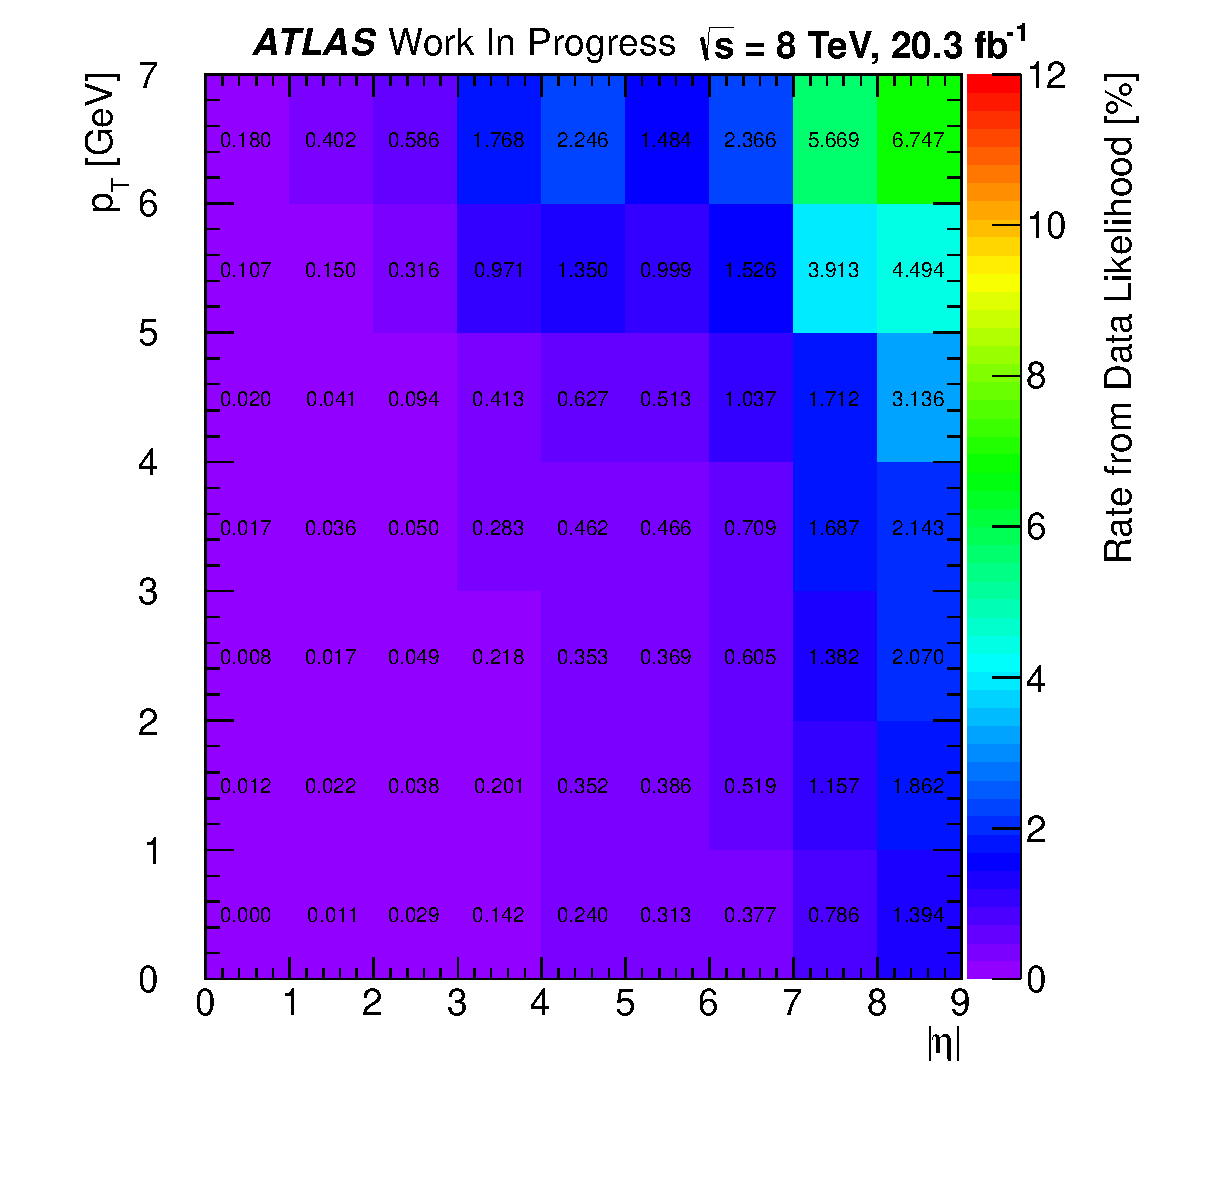
\includegraphics[width=0.45\columnwidth]{figures/ChargeMisID/Nov5_2015_DataRates_Plot.eps}
\caption{Electron charge mis-identification rates as a function of
the electron \pt and $\eta$ extracted using the MC
truth method (left) and the likelihood method in data (right). }
\label{fig:chargemisid_rates_contour}
\end{figure}

The rates for the two different methods are 
shown in \fig\ref{fig:chargemisid_rates_contour}.
For low values of \pt and $\eta$, the rate is small enough to be negligible. 
The rate increases gradually along both dimensions, reaching as much as
6.7\% in the region $\pt > 120\GeV$ and $2.4 < |\eta| < 2.5$ as measured
in the data, which corresponds to the highest bin in both dimensions. 
The rates measured using MC truth information are systematically higher
than those measured in data, almost by a factor of two. The MC simulation
tends to overestimate the amount of material (figure?) actually in the
detector, which could explain this difference....
%figure 4.45 in jinst?
%or maybe https://atlas.web.cern.ch/Atlas/GROUPS/PHYSICS/PAPERS/PERF-2013-05/
%or https://atlas.web.cern.ch/Atlas/GROUPS/PHYSICS/PAPERS/PERF-2013-03/
%might it be that the material description was improved in a later version of the MC?
%mc12b is known to have a maybe 20-30% lower rate of photon conversions overall
%according to Jake, I guess because of the material description.
%could the imporved simulation referred to in one of the papers above
%be for something that was included after mc12b? probably
%ruiqi used this sample for the MC generation:
%mc12 8TeV.147806.Powheg Pythia8 AU2CT10 Zee.merge.NTUP COMMON.e1169 s1469 s1470 r3542 r3549 p1562
%this twiki
%https://twiki.cern.ch/twiki/bin/view/Atlas/MC12cWiki?rev=3
%claims that improvements to the geometry came in mc12c
%However, these improvements claim that the improved geometry
%describes more material at high eta. It seems like this would only 
%make the disagreement between the mc and data rates, assuming
%that more material really does cause more conversion
%the paper claims the difference is in part to an incomplete
%description of SCT cooling pipes.
%the most discrepant region is between eta of 1.4 and 1.6, where the 
%difference would be consistent if material were removed.
%but this then would seem to suggest that the differences show up mostly
%in eta bin 3, which they do not. Instead it grows starting
%for eta > 2.0




%note: the material description shouldn't be affecting our zgamma
%estimate since it requires a b-layer hit so these are converting early

Some additional alternatives to these two methods are also performed
in order to better assess the performance of the mehtods
and to determine systematic uncertainties.
One alternative is to perform the same likelihood extraction
as in the data, but using only reconstructed MC. This produces
similar rates to the truth MC method, suggesting that the differences
seen between the data likelihood method and the truth MC method
are not due to the method itself. 

Another method is to extract the rates from the data with the 
likelihood method but without performing the background
subtraction mentioned earlier. In the original method, 
the background subtraction is performed by... 
...with a template fit like in \fig\ref{fig:chargemisid_fitexample}.

\begin{figure}[htp]
\centering
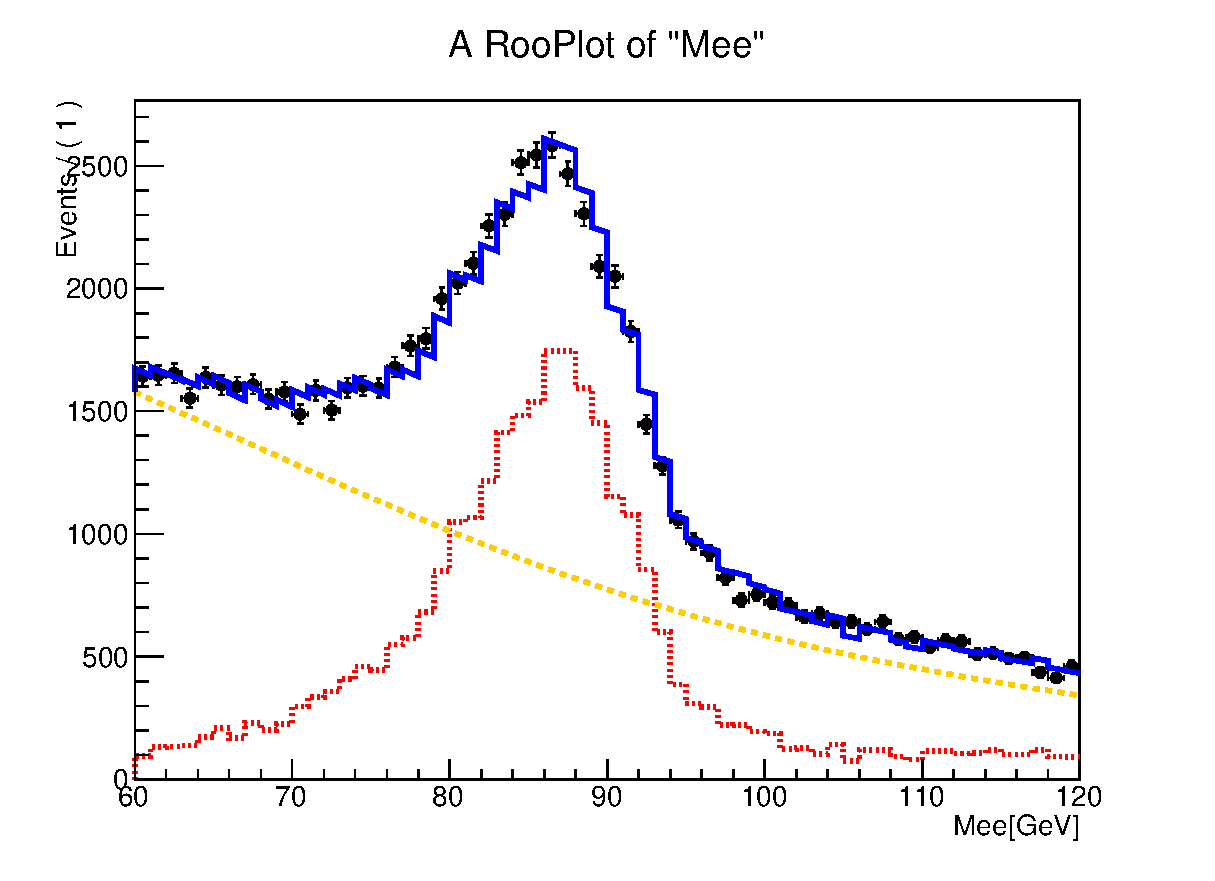
\includegraphics[width=0.6\textwidth]{figures/ChargeMisID/Tot_Polynomial_0_2.eps}
\caption{Plot of the di-lepton invariant mass 
in the region where one electron has $0 < |\eta_1| < 0.8$
and the other has $1.15 < |\eta_2|<1.6$. The data (black points)
are shown in a region where the electron isolation cuts are removed
and the electron quality requirements are loosened.
A template from $Z\rightarrow ee$ MC (red line) and a polynomial
curve (orange line) are used to fit the data. The sum of the fit
(blue line) is seen to fit the data well.}
\label{fig:chargemisid_fitexample}
\end{figure} 


The different methods of rate estimation are compared to extract
a final systematic. In \fig\ref{fig:ChargeMisID_truthRate_finalFig},
the two-dimensional rates are unfolded into one-dimension
with the bins numbered counting from low values of $\eta$ and \pt~to
high values. The nominal rate is the one shown as black points
using a likelihood fit in data with background subtraction. The vertical
bars on the black points show the statistical uncertainty on this method.
The solid black line shows the same method but without background subtraction.
These methods follow eachother quite closely, uniformly differing by 
5-6\% throughout.  The blue curve shows the rates evaluated
using the MC truth method. As was already mentioned, these tend
to be larger than the rates in data by about a factor of two. Finally, 
the red curve shows the rates evaluated using the same likelihood method
applied to the data, but using only reconstructed MC. This is seen to follow
closely the MC truth method closely, except in a few bins where the statistics
are low. The relative difference between the MC truth and MC likelihood methods
is transported to the nominal estimate in data and used as another systematic.
The difference between the methods using data and those using MC is not
used as a systematic since such a difference is expected.
The systematic uncertainties are combined in quadrature with the statistical
uncertainty on the nominal estimate to arrive at a final uncertainty on the
rates, shown as a hashed band.


\begin{figure}[htp]
\centering
\includegraphics[width=0.9\textwidth]{figures/ChargeMisID/Validation_ChargeMisIDRates_PTvsEta_FinalRateWithSys.png}
\caption{Summary of electron charge mis-identification rates using
the likelihood method in data with background subraction (black points) 
and without background subtraction (black line), the MC truth 
method (blue line), and the likelihood method in MC (red).
Systematic uncertainties are extracted as described in the text and are shown
in the gray hashed band pointing from bottom left to top right. 
The systematic uncertainties are combined with the statistical uncertainties
on the black points to arrive at a total uncertainty on the rates, shown 
in the hashed band pointing from bottom right to top left.}
\label{fig:ChargeMisID_truthRate_finalFig}
\end{figure}




\subsubsection{Di-boson MC Reweighting}


The electron charge mis-identification  rates are primarily important for the determination of the $WZ$ and $ZZ$ background contamination in the 0 SFOS region,
as mentioned already.
Once derived, the rates are applied to $WZ$ and $ZZ$ MC samples based on 
whether or not a charge flip could cause the event to appear in the 0 SFOS region.  
In particular, the following di-boson decays are considered:
\begin{itemize}
\item $WZ\rightarrow e^{\pm}\nu~ e^{+}e^{-}$
\item $WZ\rightarrow \mu^{\pm}\nu~ e^{+}e^{-}$
\item $WZ\rightarrow \tau^{\pm}\nu~ e^{+}e^{-}$
\item $ZZ\rightarrow e^{+}e^{-}~e^{+}e^{-}$
\item $ZZ\rightarrow \mu^{+}\mu^{-}~ e^{+}e^{-}$
\end{itemize}
No other decay channels are considered.  These all share in common that they 
have at least one electron-positron pair.  
Except for the $WZ\rightarrow \tau^{\pm}\nu~e^{+}e^{-}$ decay channel, 
decay channels with tau leptons are not considered
because they are suppressed by the tau branching fraction and are 
considered to be negligible.

The charge mis-identification rates are then applied to these channels on an 
event-by-event basis as follows.
For each event that is processed, its decay channel is identified 
at truth level. Each reconstructed lepton
is examined  and assigned a rate, or a probability to charge flip, 
based on its reconstructed $\pt$ and $\eta$ values.
The probability for a charge flip to occur in an event is then approximately 
the sum of rates for the individual electrons:
\begin{equation}
p(\textrm{Charge Mis-Identification in Event}) \approx \sum_{i \in \textrm{Electrons}}  \textrm{Rate}(\pt^i,\eta^i) 
\end{equation}
Higher order terms where multiple electrons are charge mis-identified is 
small and considered to be negligible.
We are only concerned with the probability that a charge flip results in the 
event falling into the 0 SFOS region. 
Consider a step function, $\Theta(e)$, defined for an individual event:
\[
\Theta(e) = 
\begin{cases}
\hfill 1 \hfill & \text{if flipping charge of $e$ classifies event as 0 SFOS} \\
\hfill 0 \hfill & \text{if flipping charge of $e$ does NOT classify event as 0 SFOS}\\
\end{cases}
\]
Then the probability that a charge mis-identification occurs and results in 
the event falling in the 0 SFOS region is:
\begin{equation}
p(\textrm{Event is classified as 0 SFOS}) \approx \sum_{i \in \textrm{Electrons}}  \textrm{Rate}(\pt^i,\eta^i)\Theta(i) 
\end{equation}
Again, we ignore the case where multiple electrons have their charge 
mis-identified.  This probability is then used as an event by event weight. 


Once the weight has been determined, we then artificially flip the charge of 
one of the electrons/positrons in the event.
If there is only one electron in the event that will lead the event 
to fall in the 0 SFOS region, its charge is flipped
and one proceeds to the next event.  However, if there are multiple electrons 
in the event, there is an ambiguity that must be resolved
about which electron's charge should be flipped. One must then be careful in 
this case to not introduce any bias.
We decided to choose a procedure where we pick a single electron from the 
event at random based on the charge flip rates
of the individual electrons. Thus, for an individual electron in an 
event, the probability that it is chosen to have its charge
flipped is:
\begin{equation}
p(\textrm{$e$ has been charge flipped}) = \textrm{Rate}(\pt^e,\eta^e)\Theta(e)~/\sum_{i \in \textrm{Electrons}} \textrm{Rate}(\pt^i,\eta^i)\Theta(i)
\end{equation}

Consider an example where the event under consideration comes from the 
decay $WZ\rightarrow e^{+}\nu e^{+}e^{-}$. Assume all three charged leptons 
pass reconstruction and are selected then label 
them as: $e^{+}_1~e^{+}_2e^{-}_3$. In this case,
the only way that this event could be classified as 0 SFOS when 
flipping the charge of only one electron/positron is to flip the 
charge of the electron.
Thus, $\Theta(e^{+}_1)=\Theta(e^{+}_2)=0$ and $\Theta(e^{-}_3)=1$.  The event 
weight will then be equal to the rate of charge mis-identification 
for  $e^{-}_3$ and it will have it's charge flipped to be positive.

Now consider an example of an event with 
the decay of $ZZ\rightarrow \mu^{+}\mu^{-}~ e^{+}e^{-}$.
If all four leptons are reconstructed and selected, the event will not 
be considered at all in the three lepton selection of this analysis, so 
consider the case where the $\mu^{+}$ is not selected leaving three leptons 
labeled as: $\mu^{-}_1 e^{+}_2 e^{-}_3$.  The probability for the muon to 
charge flip is negligible which leaves the electron and the positron. Flipping 
the charge of either one at a time will result in the event being 
classified as 0 SFOS.  Thus, in
this case $\Theta(\mu^{-}_1)=0$ and $\Theta(e^{+}_2)=\Theta(e^{-}_3)=1$. The 
event weight will then be the sum of the rates for $e^{+}_2$ and $e^{-}_3$.
The probability that the electron has its charge flipped is then 
$\frac{\textrm{Rate}(e^{-}_3) }{ \textrm{Rate}(e^{+}_2)+ \textrm{Rate}(e^{-}_3)}$ 
and similarly for the positron.

\subsubsection{Validation}
This procedure has been validated on the $WZ$ and $ZZ$ samples by comparing 
the predictions taken directly from MC to the predictions reweighted in the 
0 SFOS signal region using the procedure just described. This is done in 
Figure~\ref{fig:ChargeMisID_Validation_WZ} for the $WZ$ samples and on 
Figure~\ref{fig:ChargeMisID_Validation_ZZ} for the $ZZ$ samples. It can be seen 
the agreement in the shape looks good for all the distributions. An offset 
between the two distributions is observed. This difference is covered partially by 
the systematic uncertainties of the method.  Any remaining difference could 
be expected from the difference in rates observed at high $\eta$ and 
high $E_{T}$ as seen in Fig.~\ref{fig:ChargeMisID_truthRate_finalFig} and 
serves as justification for using the data-driven method.

There is no special treamtent of the charge mis-identification contribution to 
other background contributions in the 0 SFOS region or to any contributions to the 
1 and 2 SFOS signal regions, including diboson processes, as the effect is 
expected to be very small.  Any charge mis-identification events are thus 
taken directly from MC in this case.


 \begin{figure}[htp]
 \centering
 \includegraphics[width=0.4\textwidth]{figures/ChargeMisID/Validation_ChargeMisIDRates_WZ_PTLepton.png}
 \includegraphics[width=0.4\textwidth]{figures/ChargeMisID/Validation_ChargeMisIDRates_WZ_EtaLepton.png}
 \includegraphics[width=0.4\textwidth]{figures/ChargeMisID/Validation_ChargeMisIDRates_WZ_DeltaPhi.png}
 \includegraphics[width=0.4\textwidth]{figures/ChargeMisID/Validation_ChargeMisIDRates_WZ_MET.png}
 \includegraphics[width=0.4\textwidth]{figures/ChargeMisID/Validation_ChargeMisIDRates_WZ_Mee.png}
 \includegraphics[width=0.4\textwidth]{figures/ChargeMisID/Validation_ChargeMisIDRates_WZ_JetMultiplicity.png}

 \caption{Validation of the charge mis-ID rates comparing 
 MC $WZ\rightarrow \ell ee$ ($\ell=e,\mu$) samples reweighted with the 
 charge misID rates measured in the MC $Z\to{}ee$ 
 sample to the original MC predictions. Distribution of 
 lepton $p_{T}$, $\eta$, $\Delta \phi(3l,E_{T}^{Miss})$,\met{}, Same-sign 
 di-electron invariant mass, and jet multiplicity.}
 \label{fig:ChargeMisID_Validation_WZ}
 \end{figure}
 
 
 \begin{figure}[htp]
 \centering
 \includegraphics[width=0.4\textwidth]{figures/ChargeMisID/Validation_ChargeMisIDRates_ZZ_PTLepton.png}
 \includegraphics[width=0.4\textwidth]{figures/ChargeMisID/Validation_ChargeMisIDRates_ZZ_EtaLepton.png}
 \includegraphics[width=0.4\textwidth]{figures/ChargeMisID/Validation_ChargeMisIDRates_ZZ_DeltaPhi.png}
 \includegraphics[width=0.4\textwidth]{figures/ChargeMisID/Validation_ChargeMisIDRates_ZZ_MET.png}
 \includegraphics[width=0.4\textwidth]{figures/ChargeMisID/Validation_ChargeMisIDRates_ZZ_Mee.png}
 \includegraphics[width=0.4\textwidth]{figures/ChargeMisID/Validation_ChargeMisIDRates_ZZ_JetMultiplicity.png}

 \caption{Validation of the charge mis-ID rates comparing 
 MC $ZZ\rightarrow \ell \ell ee$ ($\ell=e,\mu$) samples reweighted with the 
 charge misID rates measured in the MC $Z\to{}ee$ 
 sample to the original MC predictions. Distribution of 
 lepton $p_{T}$, $\eta$, $\Delta \phi(3l,E_{T}^{Miss})$,\met{}, Same-sign 
 di-electron invariant mass, and jet multiplicity.}
 \label{fig:ChargeMisID_Validation_ZZ}
 \end{figure}



  
\subsection{Fake lepton background}
\label{sec:bg_fake}
\subsection{Fake lepton background}
\label{sec:bg_fake}

This background consists of the events with at least one non-prompt lepton denoting the hadrons misidentified as leptons and leptons originating from heavy-flavour decays, such as $b-$meson decays. We refer to these non-prompt leptons as ``fake'' leptons and subsequently refer to prompt leptons as ``real'' leptons. It is estimated using a generalised matrix method \cite{Arguin:1558979,Gillam:2014xua} which is a fully data-driven technique. All leptons are firstly classified as ``loose'' or ``tight'' according to their identification and/or isolation quality. The loose leptons must pass all lepton preselection requirements and fail any of the signal selection criteria defined in Tables \ref{tab:eledef} and \ref{tab:muondef}. Once the efficiencies for real and fake preselected leptons to satisfy the tight lepton selections are measured, the number of events with fake lepton background can be predicted. This measurement is done as a function of $\pt$. %and/or \pt\ bin.


\tabcolsep=0.11cm
\begin{table}[ph!]
\begin{center}
\small{
    \begin{tabular}{lc}
%      \hline
%      Cut            & Value/description \\
      \hline
      \hline
      \multicolumn{2}{c}{\textbf{Preselected electron}}\\
      \hline
      Algorithm      & Central Electrons (author is 1 or 3)\\
      \hline
      Acceptance     & $\pt > 10\,\GeV, |\eta| < 2.47$ excluding crack region \\
      \hline
      Quality & \texttt{Medium++} \\
%      \hline
%      Further cuts & not touching dead OTX region\\
      \hline
      Impact parameter & $|d_0/\sigma(d_0)| < 3.0$\\ 
      & $|z_0 \cdot sin(\theta)|<$ 0.5 mm \\
      \hline
      $e$-$e$ isolation             & $\Delta{}R(e,e)>0.2$ \\
      \hline
      $e$-$\mu$ isolation      & $\Delta{}R(e,\mu)>0.2$ \\
      \hline
      \multicolumn{2}{c}{\textbf{Signal electron}}\\
      \hline
      Quality & \texttt{Tight++} \\
%      \hline
%      Track   & with match \\
      \hline
      Track isolation   & \pt cone20/\pt $<0.04$\\
      \hline
      Calorimeter isolation & \ET cone20/\ET$<0.10$\\% for \pt$>20$\GeV\\
      					  % & \ET cone20/\ET$<0.07$ for \pt$<20$\GeV\\
     \hline
     \hline
\end{tabular}
}
\end{center}
\caption{Summary of the electron selection criteria used for the global matrix method. The signal requirements defined in Section~\ref{sec:Object_selection} are applied on top of the lepton preselection.}
\label{tab:eledef}
\end{table}

\tabcolsep=0.11cm
\begin{table}[ph!]
  \begin{center}%\renewcommand\arraystretch{1.2}
  \small{
    \begin{tabular}{lc}
%      \hline
 %     Cut            & Value/description \\
      \hline
      \hline
      \multicolumn{2}{c}{\textbf{Preselected muon}}\\
      \hline
      Algorithm      & STACO combined \\
      \hline
      Acceptance     & $\pt > 10\,\GeV, |\eta| < 2.5$ \\
      \hline
      Quality        & Tight    \\
      \hline
      Inner detector track quality & MCP ID Hits selection\\
      \hline
            Impact parameter & $|d_0/\sigma(d_0)| < 3.0$\\ 
      & $|z_0 \cdot sin(\theta)|<$ 0.5 mm \\
      \hline
      $\mu$-$\mu$ isolation             & $\Delta{}R(\mu,\mu)>0.2$ \\
      \hline
      \multicolumn{2}{c}{\textbf{Signal muon}}\\
      \hline
      Track isolation   & \pt cone20/\pt $<3.0$\\
      \hline
      Calorimeter isolation & \ET cone20/\ET $<0.10$\\% for \pt$>20$\GeV\\
      						%& \ET cone20/\ET $<0.07$ for \pt$<20$\GeV\\
      \hline
      \hline
    \end{tabular}
    }
  \end{center}
   \caption{Summary of the muon selection criteria used for the global matrix method. The signal requirements defined in Section~\ref{sec:Object_selection} are applied on top of the lepton preselection.} 
    \label{tab:muondef}
\end{table}

\subsubsection{Generalized matrix element method}

The advantage of the matrix method used in this analysis is that an arbitrary number of preselected leptons can be present in the event. In case of single lepton events, the equation relating the number of events with real ($n_R$) and fake ($n_F$) lepton in $\pt$ bin $i$ to the expected number of events with the lepton reconstructed as tight ($n_T$) or loose ($n_L$) can be written as following:
\begin{align*}
  \begin{pmatrix} n_T \\ n_L \end{pmatrix} 
  &= 
  \begin{pmatrix}
  \varepsilon_i & \zeta_i \\ 1-\varepsilon_i & 1-\zeta_i
  \end{pmatrix} 
  \begin{pmatrix} n_R \\ n_F \end{pmatrix}
\end{align*}
where $\varepsilon_i$ and $\zeta_i$ are the real and fake efficiencies measured in $\pt$ bin $i$. Given the measurements of $n_T$ and $n_L$, the expected real and fake contributions can be calculated from the inverted relation:
\begin{align*}
  \begin{pmatrix} n_R \\ n_F \end{pmatrix} 
  &= 
  \frac{1}{\varepsilon_i-\zeta_i}
  \begin{pmatrix}
  1-\zeta_i & -\zeta_i \\ \varepsilon_i-1 & \varepsilon_i	
  \end{pmatrix} 
  \begin{pmatrix} n_T \\ n_L \end{pmatrix}
\end{align*}
%Take an event selection requiring exactly one baseline lepton, which we additionally require to pass tight quality requirements. We have measured nT and nL, and want n'T the expected number of tight leptons that are fake.
%The procedure to obtain an estimate for the fake lepton contribution passing the tight requirements $n'_T$ in single lepton events is:
The procedure to obtain an estimate for the number of fake leptons passing the tight requirements $n'_T$ is:
\begin{align*}
  \begin{pmatrix} n'_T \\ n'_L \end{pmatrix} 
  &= 
  \begin{pmatrix}
  \varepsilon_i & \zeta_i \\ 1-\varepsilon_i & 1-\zeta_i
  \end{pmatrix} 
  \begin{pmatrix} 0 \\ n_F \end{pmatrix}
  =  
  \begin{pmatrix}
  \varepsilon_i & \zeta_i \\ 1-\varepsilon_i & 1-\zeta_i
  \end{pmatrix} 
  \begin{pmatrix}0&0\\0&1\end{pmatrix} 
  \begin{pmatrix} n_R \\ n_F \end{pmatrix}\\
  &=
  \begin{pmatrix}
  \varepsilon_i & \zeta_i \\ 1-\varepsilon_i & 1-\zeta_i
  \end{pmatrix} 
  \begin{pmatrix}0&0\\0&1\end{pmatrix} 
  \frac{1}{\varepsilon_i-\zeta_i}
  \begin{pmatrix}
  1-\zeta_i & -\zeta_i \\ \varepsilon_i-1 & \varepsilon_i	
  \end{pmatrix} 
  \begin{pmatrix} n_T \\ n_L \end{pmatrix}
\end{align*}
This is typically calculated as a weight $w_i$ for each event where the lepton in \pt\ bin $i$ is either tight ($n_T=1$ and $n_L=0$) or loose ($n_T=0$ and $n_L=1$).

For compactness, it is useful to introduce the following notation where summation convention is implied over repeated indices:
\begin{align*}
  r = \begin{pmatrix} n_R \\ n_F \end{pmatrix} , \quad
  t = \begin{pmatrix} n_T \\ n_L \end{pmatrix} , \quad
  \phi  = 
  \begin{pmatrix}
    \varepsilon_i & \zeta_i \\
    1-\varepsilon_i & 1-\zeta_i
  \end{pmatrix} 
  \quad\Rightarrow
  \quad
  t_\beta = {\phi}_\beta^{\ \alpha} r_\alpha
\end{align*}
where $\alpha$ takes values corresponding to $R$ or $F$, and similarly $\beta$ for $T$ or $L$. The expected number of tight leptons that are fake is then:
\begin{align*}
  t'_\nu = {\phi}_\nu^{\ \mu} \omega_\mu^{\ \beta} {{\phi}^{-1}}_\beta^{\ \alpha} t_\alpha
\end{align*}
where $\omega$ represents the selection of only the expected fake component. 

In case of an event with $N$ preselected leptons, the formula can be written in this compacted notation as following:
\begin{align*}
  t'_{\nu_1\cdots\nu_N} = \phi_{\nu_1}^{\ \mu_1}\cdots\phi_{\nu_N}^{\ \mu_N}\ \omega_{\mu_1\cdots\mu_N}^{\ \beta_1\cdots\beta_N}\ {\phi^{-1}}_{\beta_1}^{\ \alpha_1}\cdots{\phi^{-1}}_{\beta_N}^{\ \alpha_N} t_{\alpha_1\cdots\alpha_N}.
\end{align*}
Each $\phi$ is computed with the efficiencies $\varepsilon$ and $\zeta$ appropriate for the lepton index. The ``real/fake configuration selector'' $\omega$ picks out the sets of indices ${\beta_i}$ corresponding to components one wish to count as fake background. In general, it looks like:
\begin{align*}
  \omega_{\mu_1\cdots\mu_N}^{\ \beta_1\cdots\beta_N} = \delta_{\mu_1}^{\ \beta_1}\cdots\delta_{\mu_N}^{\ \beta_N} \ f(\beta_1,\,\ldots,\,\beta_N)
  % \omega_{\mu_1\cdots\mu_N}^{\ \beta_1\cdots\beta_N} = \delta_{\mu_1}^{\ \beta_1}\cdots\delta_{\mu_N}^{\ \beta_N} \ f(\beta_1,\,\ldots,\,\beta_N,\nu_1,\,\ldots,\,\nu_N)
\end{align*}
where $\delta_i^j$ is the Kronecker delta and $f$ is a function of the indices taking values 1 (for a fake combination) and 0 (for a real combination).
%where the function $f$ takes values 0 or 1 to pick out the sets of indices ${\beta_i}$ that correspond to components we wish to count as fake background. In general it will depend on the output tight/loose configuration being computed, and we choose it such that the number of real leptons (out of the $N$ in the event) in the intermediate configuration $\{\beta\}$ is less than the number of tight leptons in the output configuration $\{\nu\}$.

This method assigns a set of weights for each event with $N$ leptons and a measured tight/loose combination -- one for each output tight/loose configuration separately. Therefore, for each of these matrix method output combinations, different leptons will be defining the event and passing through the signal selections. It is important to stress that the correlations between each configuration must be taken into account.
%
%For each event with $N$ leptons and a measured tight/loose combination $\{\alpha\}$, this method hence gives a weight for each output tight/loose combination $\{\nu\}$. Since, for each of these combinations, different leptons will be defining the event, each combination is propagated through the final channel selection and trigger matching procedure separately, with the leptons being treated as tight or loose according to the output of the matrix method. Variables such as invariant mass of $Z$ boson are also computed using the appropriate leptons.
%
%For example, if one measures an event with three pre-selected leptons,
%$e^+e^-\mu^+$, with configuration TLL, then the matrix method will produce
%the following
%\begin{align*}
%  \textrm{\textbf{Input}} \qquad\qquad & \qquad\qquad\textrm{\textbf{Output}} \\
%  e^+e^-\mu^+, TLL \longrightarrow& \left\{
%  \begin{array}{ll}
%    LLL & w_{LLL} \quad e^+_Le^-_L\mu^+_L \quad \textrm{Fails cuts} \\
%    \cdots & \cdots \\
%    TTL & w_{TTL} \quad e^+_Te^-_T\mu^+_L \quad \textrm{Fails cuts} \\
%    TLT & w_{TLT} \quad e^+_Te^-_L\mu^+_T \quad \textrm{Fails cuts} \\
%    LTT & w_{LTT} \quad e^+_Le^-_T\mu^+_T \quad \textrm{Fails cuts} \\
%    TTT & w_{TTT} \quad e^+_Te^-_T\mu^+_T \quad \textrm{Exactly 3 leptons with 1SFOS}
%  \end{array}
%  \right.
%\end{align*}
%Of the possible combinations, only one passes the signal selection cuts,
%presuming trigger matching, $b$-jet veto and other requirements are also satisfied.

For example, if one measures an event with four preselected leptons,
$e^+e^-e^+\mu^+$, with configuration TTLL, then the matrix method will produce
the following:
\begin{align*}
  \textrm{\textbf{Input}} \qquad\qquad & \qquad\qquad\textrm{\textbf{Output}} \\
  e^+e^-e^+\mu^+, TTLL \longrightarrow& \left\{
  \begin{array}{ll}
    LLLL & w_{LLLL} \quad e^+_Le^-_Le^+_L\mu^+_L \quad \textrm{Fails cuts} \\
    \cdots & \cdots \\
    TTTL & w_{TTTL} \quad e^+_Te^-_Te^+_T\mu^+_L \quad \textrm{Exactly 3 leptons with 2SFOS} \\
    TTLT & w_{TTLT} \quad e^+_Te^-_Te^+_L\mu^+_T \quad \textrm{Exactly 3 leptons with 1SFOS} \\
    TLTT & w_{TLTT} \quad e^+_Te^-_Le^+_T\mu^+_T \quad \textrm{Exactly 3 leptons with 0SFOS} \\
    LTTT & w_{LTTT} \quad e^+_Le^-_Te^+_T\mu^+_T \quad \textrm{Exactly 3 leptons with 1SFOS} \\
    TTTT & w_{TTTT} \quad e^+_Te^-_Te^+_T\mu^+_T \quad \textrm{Fails cuts}
  \end{array}
  \right.
\end{align*}
If one presumes that trigger matching and other requirements are satisfied, only four of all possible combinations pass the event pre-selection cuts. In addition, each of these ``subevents'' falls into specific channel according to the number of same flavour opposite sign (SFOS) pairs.

To propagate uncertainties on the efficiencies, the derivatives of $t'_{\nu_1\cdots\nu_N}$ with respect to $\varepsilon_i$ and $\zeta_i$ for each lepton $i$ need to be calculated. This can be evaluated exactly and efficiently at runtime. Correlations between the real efficiencies $\varepsilon$ measured in different  $\pt$ bins are neglected since the uncertainty on the measurement is small. Correlations between the fake efficiencies $\zeta$ binned in \pt\ are preserved by propagating the systematic variation for each bin separately. Finally, there is a statistical correlation between two output configurations from one input event falling into one signal region which need to be taken into account. Using the previous example, the variance of each subevent in 1SFOS treated as separately is $w^2_{TTLT}$ and $w^2_{LTTT}$. However, it should be in fact $(w_{TTLT} +w_{TTLT})^2$. %for a signal region 1SFOS

\subsubsection{Real lepton efficiency}

The efficiencies for real preselected leptons to pass the tight requirements are measured in data as a function of the lepton $\pt$. The measurement is performed in data samples enriched with real leptons from $Z\rightarrow l^+l^-$ decay with a standard tag-and-probe method. The tag passes all signal lepton selections and is trigger matched, while the requirement imposed to the probe is to satisfy only the lepton preselection cuts. Their invariant mass has to be within $Z$-mass window: $m_{ll}\in[80, 100]$~\GeV{}. If both leptons satisfy the tag requirements, they are alternatively considered as the tag in order to avoid any bias introduced by its selection. The invariant mass for two opposite sign same-flavour leptons is illustrated in Fig. \ref{fig:realEff_CRs}.

The $\pt$ distributions for both the number of probes passing the signal requirements, $n^{\mathrm{Tight}}$, and the total number of probes, $n$, are shown separately in the electron and muon control regions used to derive the rates in Figure~\ref{fig:realEff_CRsPt}.
The efficiency, $\varepsilon_i$, is calculated in each $\pt$ bin, $i$, by taking the ratio of $n_{i}^{\mathrm{Tight}}$ over $n_i$. That is,
\begin{align*}
%\varepsilon_i=\frac{n_T^{\mathrm{probe}}}{n^{\mathrm{probe}}}
\varepsilon_i=\frac{n_{i}^{\mathrm{Tight}}}{n_{i}}
\end{align*}
The final binning of the efficiency is chosen to be coarse enough
to have good statistics in the ratio while also preserving shape information as a function
of $\pt$. 
The final efficiencies determined using both data and MC 
can be seen in Fig. \ref{fig:realEff}.

Two sources of systematic uncertainties are taken into account. Firstly, the measurement may be affected by the selection of $20$~\GeV\ $Z$-mass window. It has been thus varied by $5$~\GeV\ and the final effect has been proved to be negligible. Secondly, the measurement is done in Drell-Yan data without any  specific treatment of the other background. Therefore, the difference between the efficiencies measured in data and MC is taken as a systematic.  A summary of the rates measured in
data and MC used to compute the systematic uncertainties are shown for electrons
in Table~\ref{table:realEff_El} and for Muons in Table~\ref{table:realEff_Mu}.

\begin{figure}[h!]
\centering
\subfigure{
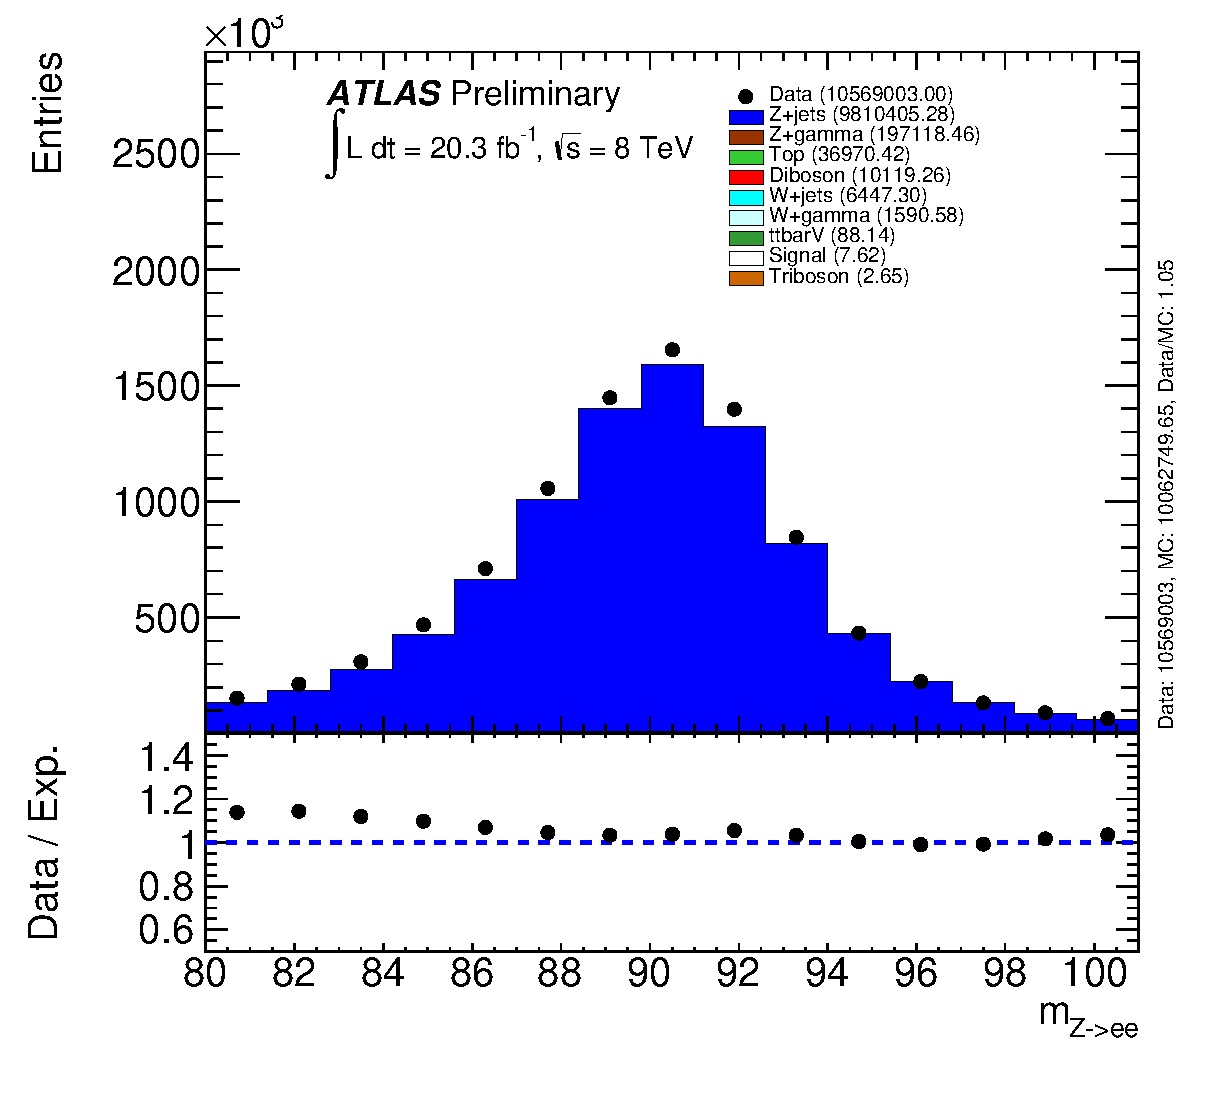
\includegraphics[width=0.4\columnwidth]{figures/fakes_bkg/CRs/hPtElectronZBosonloosecut_total_new.eps}
}
\centering
\subfigure{
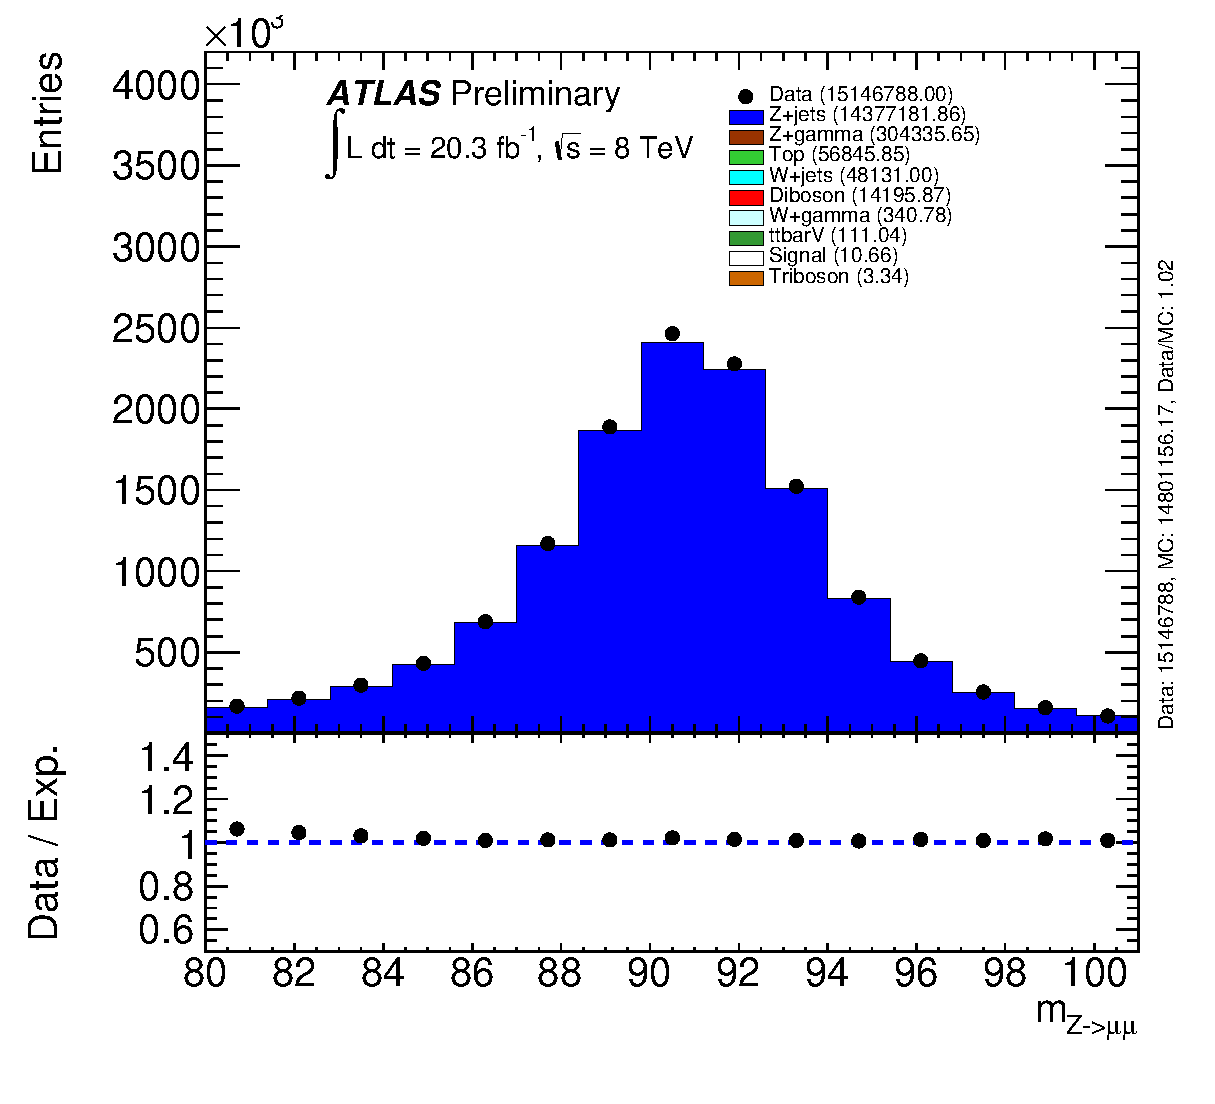
\includegraphics[width=0.4\columnwidth]{figures/fakes_bkg/CRs/hPtMuonZBosonloosecut_total_new.eps}
}
\vspace{-10mm}\caption{Invariant mass distribution of two opposite charge and same flavor di-lepton invariant mass electrons (left) and muons (right).}
\label{fig:realEff_CRs}
\end{figure}


\begin{figure}[h!]
\centering
\includegraphics[width=0.4\columnwidth]{figures/fakes_bkg/CRs/RealTP/ProbeTightElectronPt_histratio.png}
\includegraphics[width=0.4\columnwidth]{figures/fakes_bkg/CRs/RealTP/ProbeTightMuonPt_histratio.png}
\includegraphics[width=0.4\columnwidth]{figures/fakes_bkg/CRs/RealTP/ProbeElectronPt_histratio.png}
\includegraphics[width=0.4\columnwidth]{figures/fakes_bkg/CRs/RealTP/ProbeMuonPt_histratio.png}
\caption{Probe lepton \pt\ distributions in SFOS tag and probe control regions used to derive real rates.  Electron (left) and muon (right) are shown
when the probe lepton is either tight (top) or no additional selection (besides the preselection) is required (bottom)}
\label{fig:realEff_CRsPt}
\end{figure}


\begin{figure}[h!]
\centering
\includegraphics[width=0.45\columnwidth]{figures/fakes_bkg/Efficiencies/ElectronRealRates.png}
\includegraphics[width=0.45\columnwidth]{figures/fakes_bkg/Efficiencies/MuonRealRates.png}
\caption{Real lepton efficiency as a fucntion of \pt\ and measured in data (red) and MC (blue) for electrons (left) and muons (right).}
\label{fig:realEff}
\end{figure}

\clearpage

%\tabcolsep=0.11cm
\begin{table}[h!]
\centering
\begin{tabular}{|l||c|c||c|c||c|}
\hline
&\multicolumn{2}{c||}{Data}&\multicolumn{2}{c||}{MC}&\multicolumn{1}{c|}{}\\ & $\varepsilon_r$ & $\sigma_{stat}$ & $\varepsilon_r$ & $\sigma_{stat}$ & $\sigma_{sys}$\\ 
\hline\hline
%$p_{T}\in[10,15]$ GeV &  $0.6285$ &  $0.0034$ &  $0.6420$ &  $0.0036$ &  $0.0135$\\ 
%$p_{T}\in[15,20]$ GeV &  $0.6960$ &  $0.0024$ &  $0.7056$ &  $0.0025$ &  $0.0096$\\ 
$p_{T}\in[20,30]$ GeV &  $0.8105$ &  $0.0011$ &  $0.8134$ &  $0.0013$ &  $0.0028$\\ 
$p_{T}\in[30,50]$ GeV &  $0.8732$ &  $0.0005$ &  $0.8794$ &  $0.0006$ &  $0.0062$\\ 
$p_{T} > 50$ GeV &  $0.9097$ &  $0.0012$ &  $0.9150$ &  $0.0012$ &  $0.0053$\\ 
\hline
\end{tabular}

\caption{Measured real efficiencies for electrons including statistical and systematic absolute uncertainties. 
Systematic is calculated by taking the difference
between the efficiencies measured in data and MC.  The efficiency measured in data is used as the nominal central value.
} 
\label{table:realEff_El}
\end{table} 

%\tabcolsep=0.11cm
\begin{table}[h!]
\centering
\begin{tabular}{|l||c|c||c|c||c|}
\hline
&\multicolumn{2}{c||}{Data}&\multicolumn{2}{c||}{MC}&\multicolumn{1}{c|}{}\\ & $\varepsilon_r$ & $\sigma_{stat}$ & $\varepsilon_r$ & $\sigma_{stat}$ & $\sigma_{sys}$\\ 
\hline\hline
%$p_{T}\in[10,15]$ GeV &  $0.8684$ &  $0.0033$ &  $0.8763$ &  $0.0036$ &  $0.0079$\\ 
%$p_{T}\in[15,20]$ GeV &  $0.8906$ &  $0.0024$ &  $0.8956$ &  $0.0025$ &  $0.0050$\\ 
$p_{T}\in[20,30]$ GeV &  $0.9217$ &  $0.0010$ &  $0.9291$ &  $0.0012$ &  $0.0074$\\ 
$p_{T}\in[30,50]$ GeV &  $0.9700$ &  $0.0004$ &  $0.9737$ &  $0.0006$ &  $0.0038$\\ 
$p_{T} > 50$ GeV &  $0.9862$ &  $0.0011$ &  $0.9878$ &  $0.0011$ &  $0.0017$\\ 
\hline
\end{tabular}

\caption{Measured real efficiencies for muons including statistical and systematic absolute uncertainties.
Systematic is calculated by taking the difference
between the efficiencies measured in data and MC.  The efficiency measured in data is used as the nominal central value.
} 
\label{table:realEff_Mu}
\end{table} 


\clearpage

\subsubsection{Fake lepton efficiency}

The fake efficiency represents the probability that a fake lepton satisfying the preselected criteria passes also the signal requirements. 
The measurement, performed separately for each $\pt$ bin, $i$, is performed in fake-enriched samples by looking at the number of probe leptons in data 
passing preselection, $n_i$, and comparing to the number which only pass also the tight
selection, $n^{Tight}_i$. Contamination from real leptons, $n^{\mathrm{Real}}_i$ and $n^{\mathrm{Tight}, \mathrm{Real}}_i$, 
and from photon converted leptons, $n^{\mathrm{PC}}_i$ and $n^{\mathrm{Tight},\mathrm{PC}}_i$, 
is corrected using MC by subtracting from the totals.  The rate is then determined as follows:
%\begin{align*}
\begin{equation}
\zeta_i=\frac{n^{\mathrm{Tight}}_i-n^{\mathrm{Tight},\mathrm{Real}}_i-n^{\mathrm{Tight},\mathrm{PC}}_i} {n_i -n^{\mathrm{Real}}_i -n^{\mathrm{PC}}_i }
\label{eq:fakerate}
\end{equation}
%\end{align*}
Since the rates depend on the fake lepton origin, the derivation is done separately for electrons and muons.     

The classification of leptons in MC as being either real or from photon conversion is performed on an event-by-event basis at truth level using the MCTruthClassifier tool~\cite{MCtruthclassifier:twiki}.  
Since this is a dilepton control region, the majority of events with a real lepton
tag and a probe lepton due to photon conversion comes from the $W\gamma$ process where the photon converted lepton is an electron.
As expected, the number of probe muons coming from photon conversion are observed to be negligible.

Efficiencies are measured from a data set enriched with one tight lepton that passes the signal lepton selections with \pt$>40$~\GeV\ and 
one fake candidate satisfying only the preselection criteria defined in tables~\ref{tab:eledef} and~\ref{tab:muondef}. Events with additional loose or tight leptons are rejected. 
The QCD background may also enter these control regions, especially in low \met\ . Therefore, an additional \met$>10$~\GeV\ requirement is introduced. 
In order to reduce the contamination from real processes like $t\bar{t}$, $WW$ and $Z$, the two leptons are required to have the same sign.
Finally, the control regions are split based on the flavor of the tag and probe leptons.  The muon rates are determined in the region
with two muons while the electron rates are determined in the region with a muon tag and an electron probe.  The choice of a muon tag 
in the region used to derive the electron rates is particularly important since allowing electron tags have a large contamination from $Z$ backgrounds.
This is true even after the same-sign requirement because of charge mis-identification.  
The charge mis-identification rate for muons is negligible
and so allows one to use the muon-muon control region for the muon rates, which has the least contamination.
This behavior can be seen in the distributions of probe muon transverse momentum in the same-sign muon-muon tag-and-probe control region used to derive
the muon fake rates shown in Fig.~\ref{fig:fakeEff_CRs_muon} while
the distributions of probe electron transverse momentum are shown in the same-sign electron-muon tag-and-probe control region used to derive
the electron fake rates shown in Fig.~\ref{fig:fakeEff_CRs_electron}.
The control regions for both electrons and muons are further split based on the number of b-tagged jets in the event, 
which has an effect on the source of the fake leptons.  In particular, requiring b-tagged jets increases the fraction
of fake leptons coming from heavy flavor. Two different sets of control regions were ultimately considered, those
with at least one b-tagged jet and those without any requirement on the presence of b-tagged jets.  The region
with at least one b-tagged jet ($N_{b-jet} > 0$) is used as the central value since it contains more heavy flavor contributions
and so compares better with the signal regions, as described later in Section~\ref{sec:fakecomposition}.  The other is used 
to determine a systematic on the composition, described later.  


A detailed breakdown of the numbers used to compute the fake rates are shown in Appendix~\ref{sec:appendix_fakebg}.
%would it be useful to show the other dilepton control regions in an appendix?

Three systematic uncertainties are considered. First, the subtraction of the processes with 
two real leptons ($t\bar{t}V$, $VV$ and $VVV$) using MC prediction introduced an uncertainty on 
their cross-sections. This effect is estimated by varying the MC normalization by $\pm 20$\%.  %should rerun with 5%
We refer to this is as the 'correlated' systematic uncertainty.
Second, given that the extraction regions and the signal regions have different kinematic selections, 
the fake leptons of different origin dominate. This kinematic dependence of fake efficiencies has been estimated 
by modifying the requirements of the sample used for the measurement. In particular, the cut thresholds 
on the $E_{T}^{Miss}$ and tag lepton $\pt$ used
for determining the dilepton control regions are varied. The $E_{T}^{Miss}$ threshold is 
varied in 5~GeV steps scanning a range of $\pm 10$~GeV around the nominal
threshold of $E_{T}^{Miss} > 10$~GeV while the $\pt$ threshold is varied in 5~GeV steps in a range of $\pm 20$~GeV 
around the nominal threshold of $\pt > 40$~GeV.  When varying the $E_{T}^{Miss}$ cut, the $\pt$ cut
is kept at the nominal threshold and vise-versa. This is referred to as the 'uncorrelated' systematic.
These are determined separtely for electrons and muons, since they use different control regions. The 'uncorrelated' and
'correlated' systematics for electrons and muons are then combined together by adding in quadrature on an event-by-event basis.
As a result the uncertainty is presented as a single systematic uncertainty on the fake electron
contribution and a separte single systematic on the fake muon contribution.
The third and final systematic contribution comes from the choice of control region, based on the number of b-tagged
jets, as described earlier.  The nominal control regions for both the electron and muon cases is when 
there is at least one b-tagged jet present.  The difference between the rates for the nominal case
and the region where no requirement is placed on the presence of b-tagged jets is chosen as a systematic.
We have determined that the difference in the composition in these two regions adequately covers the difference
in composition that may be present due to the extrapolation from the control regions to the signal regions. This is 
discussed in more detail in Section~\ref{sec:fakecomposition}.  Another set of control regions was studied
which vetos any b-tagged jets, but this was observed to give a very large difference in composition which is 
probably too conservative of an estimate to be used as a reasonable systematic.
The rates along with the statistical and systematic uncertainties are summarized in Fig.~\ref{fig:fakeEff} 
as well as in Tables \ref{table:fakeEff_El} and \ref{table:fakeEff_Mu}.
The final binning of the efficiency is chosen to be coarse enough
to have good statistics in the ratio while also preserving shape information as a function
of $\pt$. 


%\begin{figure}[h!]
%\centering
%\subfigure{
%\includegraphics[width=0.3\columnwidth]{figures/fakes_bkg/CRs/CR1N_probePt_all_total.eps}
%}
%\centering
%\subfigure{
%\includegraphics[width=0.3\columnwidth]{figures/fakes_bkg/CRs/CR2N_probePt_all_total.eps}
%}\\ 
%\vspace{-14mm}
%\subfigure{
%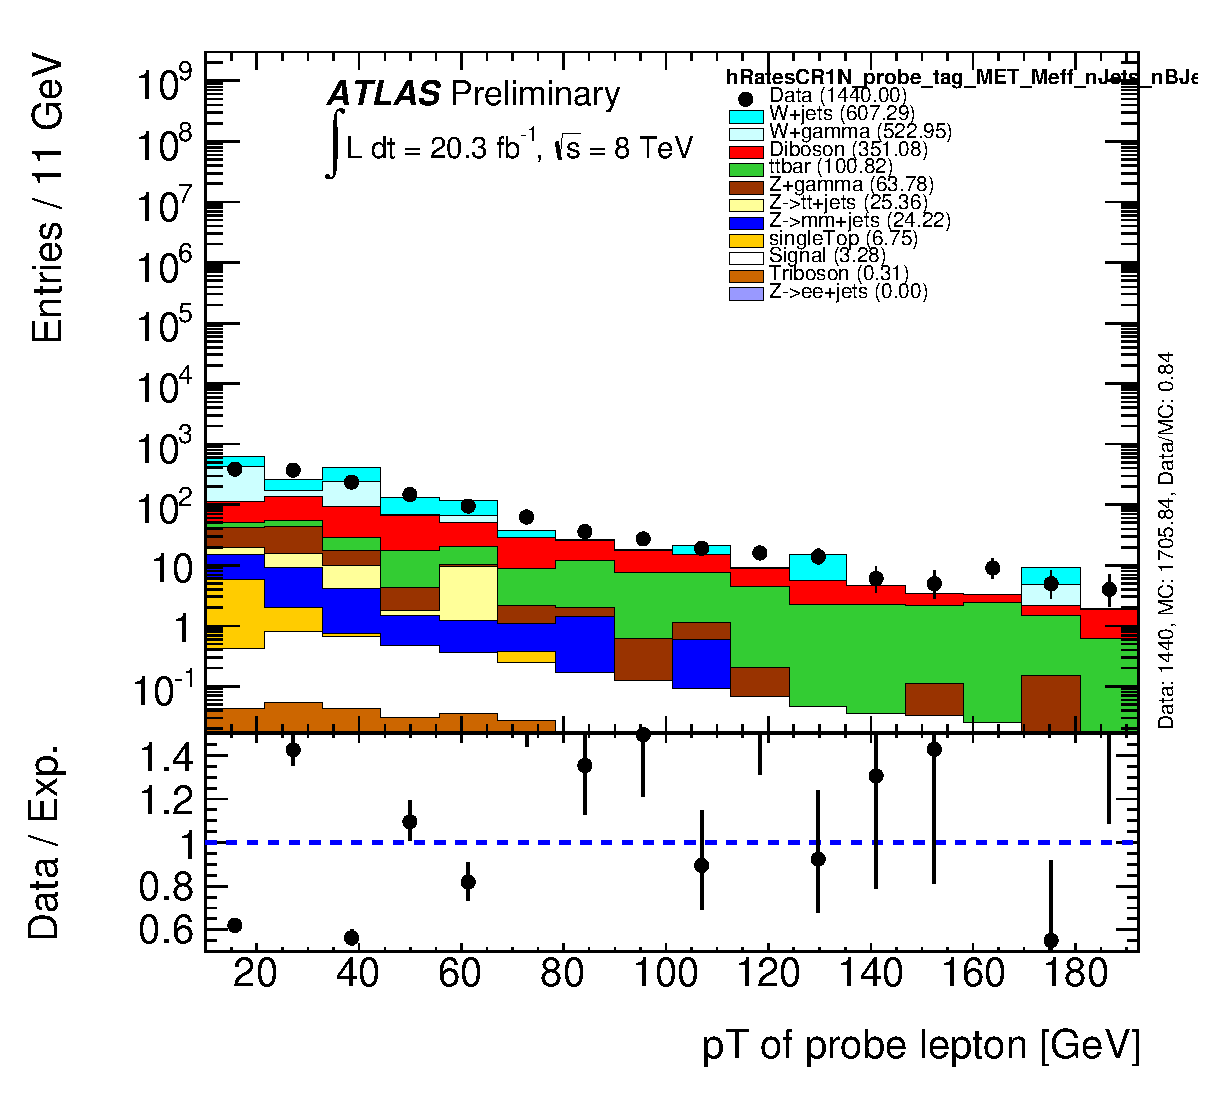
\includegraphics[width=0.3\columnwidth]{figures/fakes_bkg/CRs/CR1N_probePt_tight_total.eps}
%}
%\centering
%\subfigure{
%\includegraphics[width=0.3\columnwidth]{figures/fakes_bkg/CRs/CR2N_probePt_tight_total.eps}
%}
%\vspace{-10mm}\caption{Transverse momentum distributions \pt\ of probe electron (left) and muon (right) in the control regions. The probe passes pre-selection (top) and signal (bottom) criteria.}
%\label{fig:fakeEff_CRs}
%\end{figure}


\begin{figure}[h!]
\centering
\subfigure{
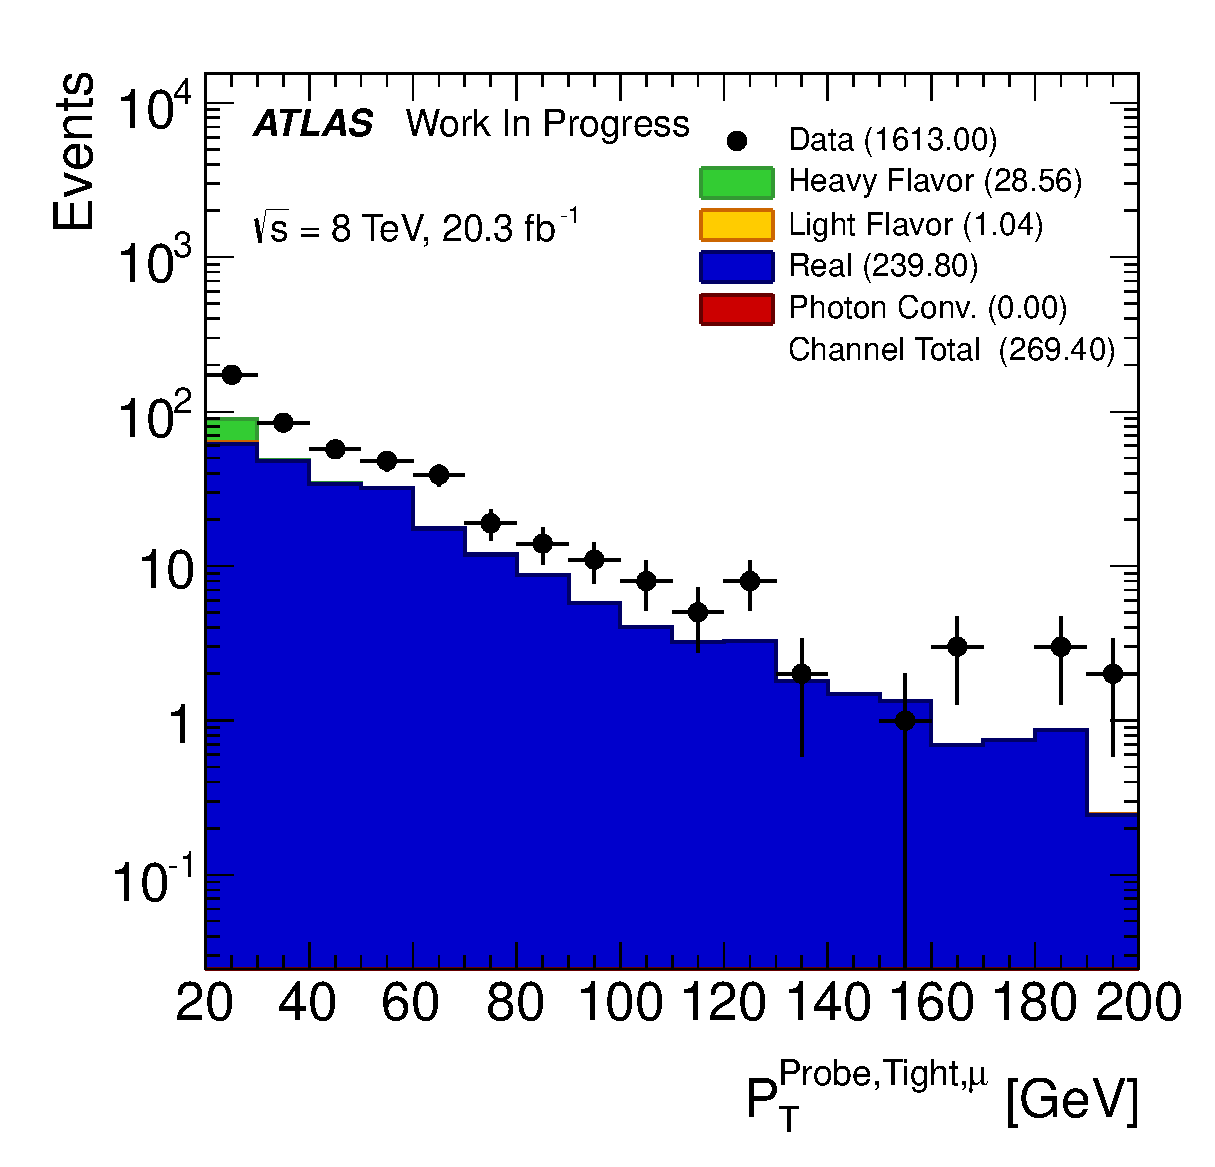
\includegraphics[width=0.45\columnwidth]{figures/fakes_bkg/CRs/SameSignMuonMuon/NoStack/ProbeTightMuonPt.eps}
}
%\centering
%\subfigure{
%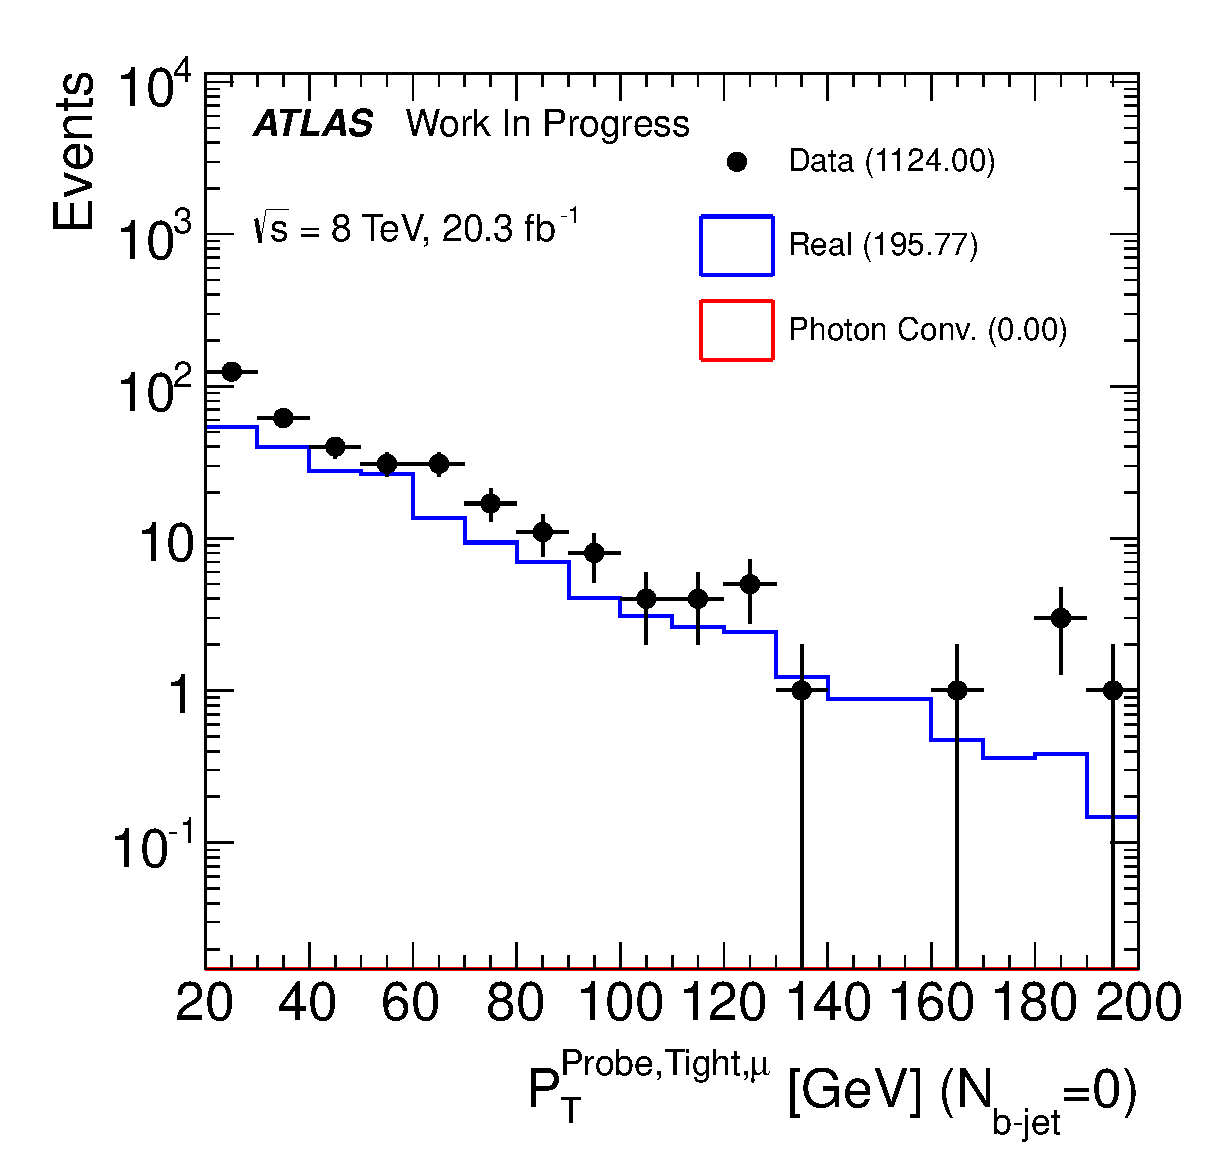
\includegraphics[width=0.3\columnwidth]{figures/fakes_bkg/CRs/SameSignMuonMuon/NoStack/ProbeTightMuonPtBJetEq0.eps}
%}
\centering
\subfigure{
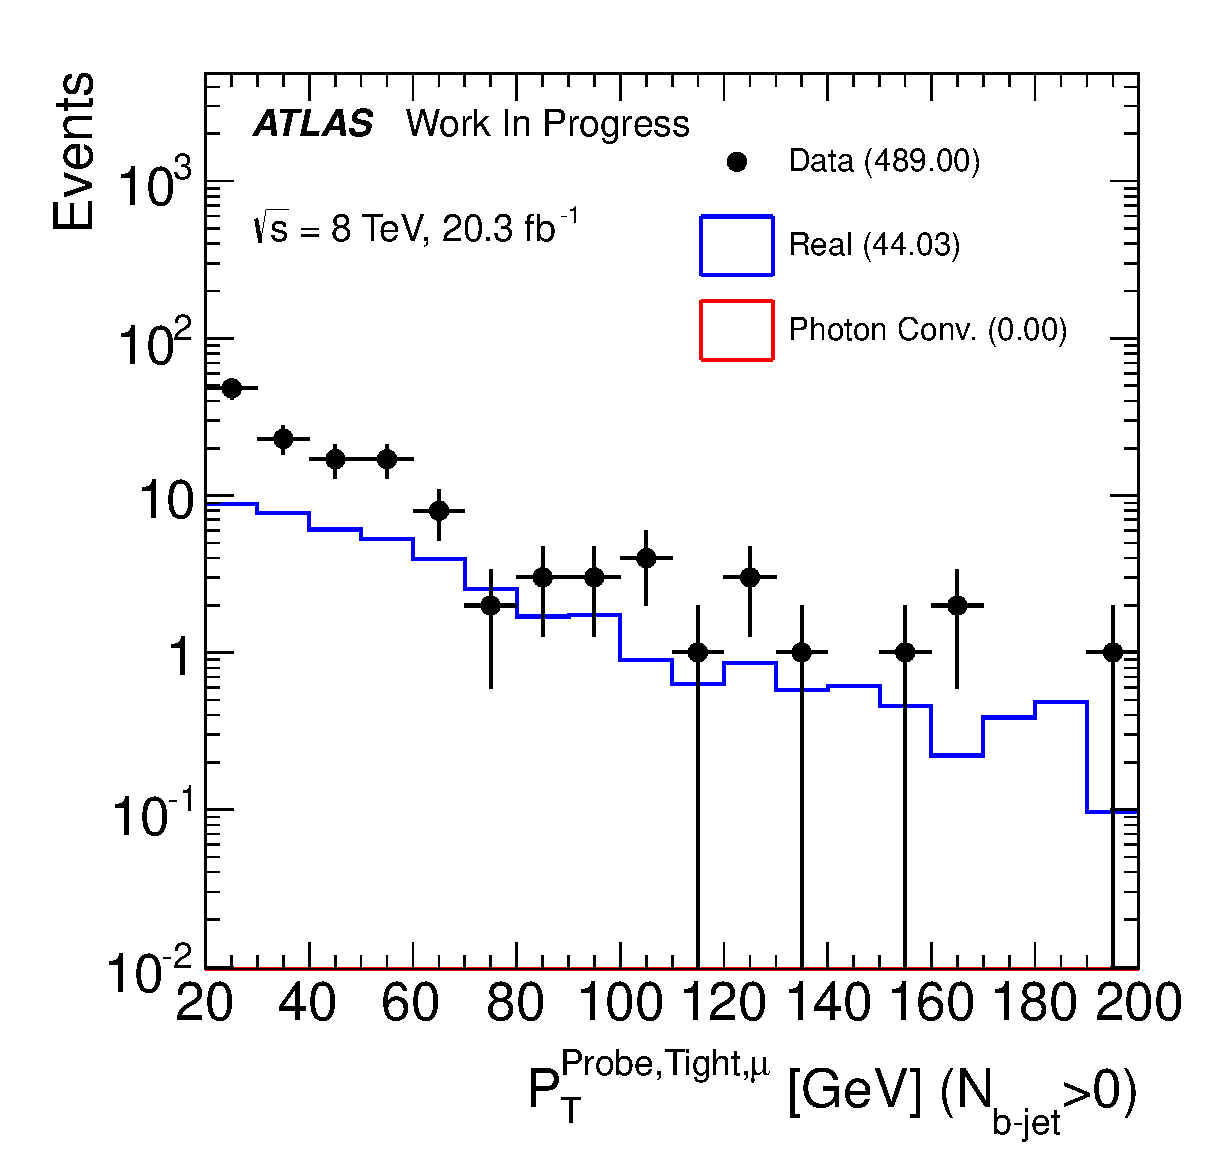
\includegraphics[width=0.45\columnwidth]{figures/fakes_bkg/CRs/SameSignMuonMuon/NoStack/ProbeTightMuonPtBJetGt0.eps}
}
%\vspace{-1mm}
\centering
\subfigure{
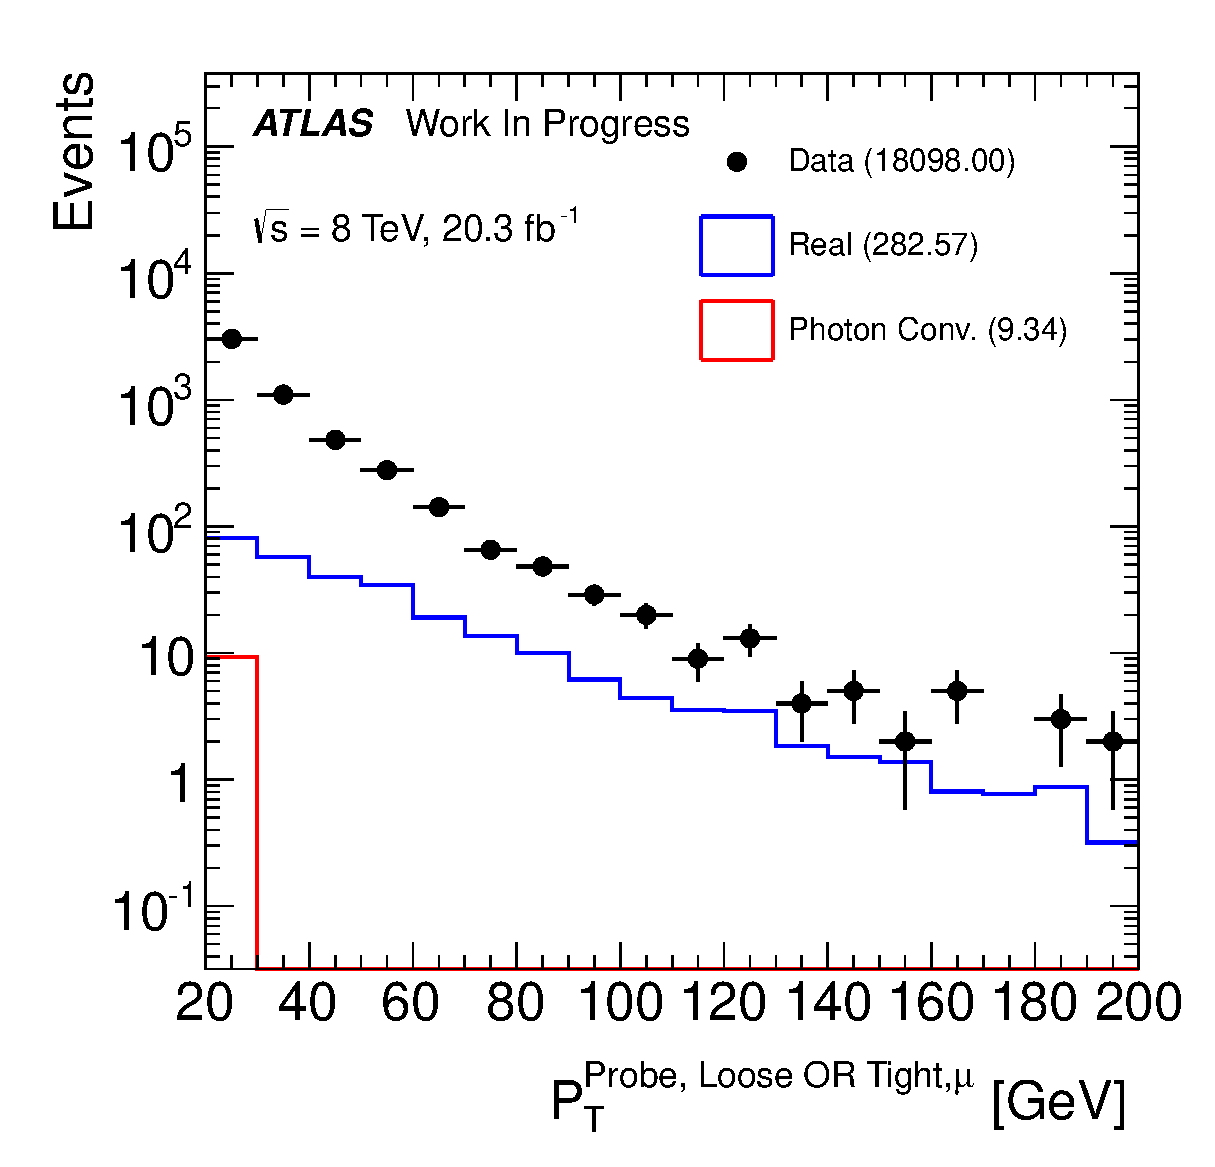
\includegraphics[width=0.45\columnwidth]{figures/fakes_bkg/CRs/SameSignMuonMuon/NoStack/ProbeLooseORTightMuonPt.eps}
}
%\centering
%\subfigure{
%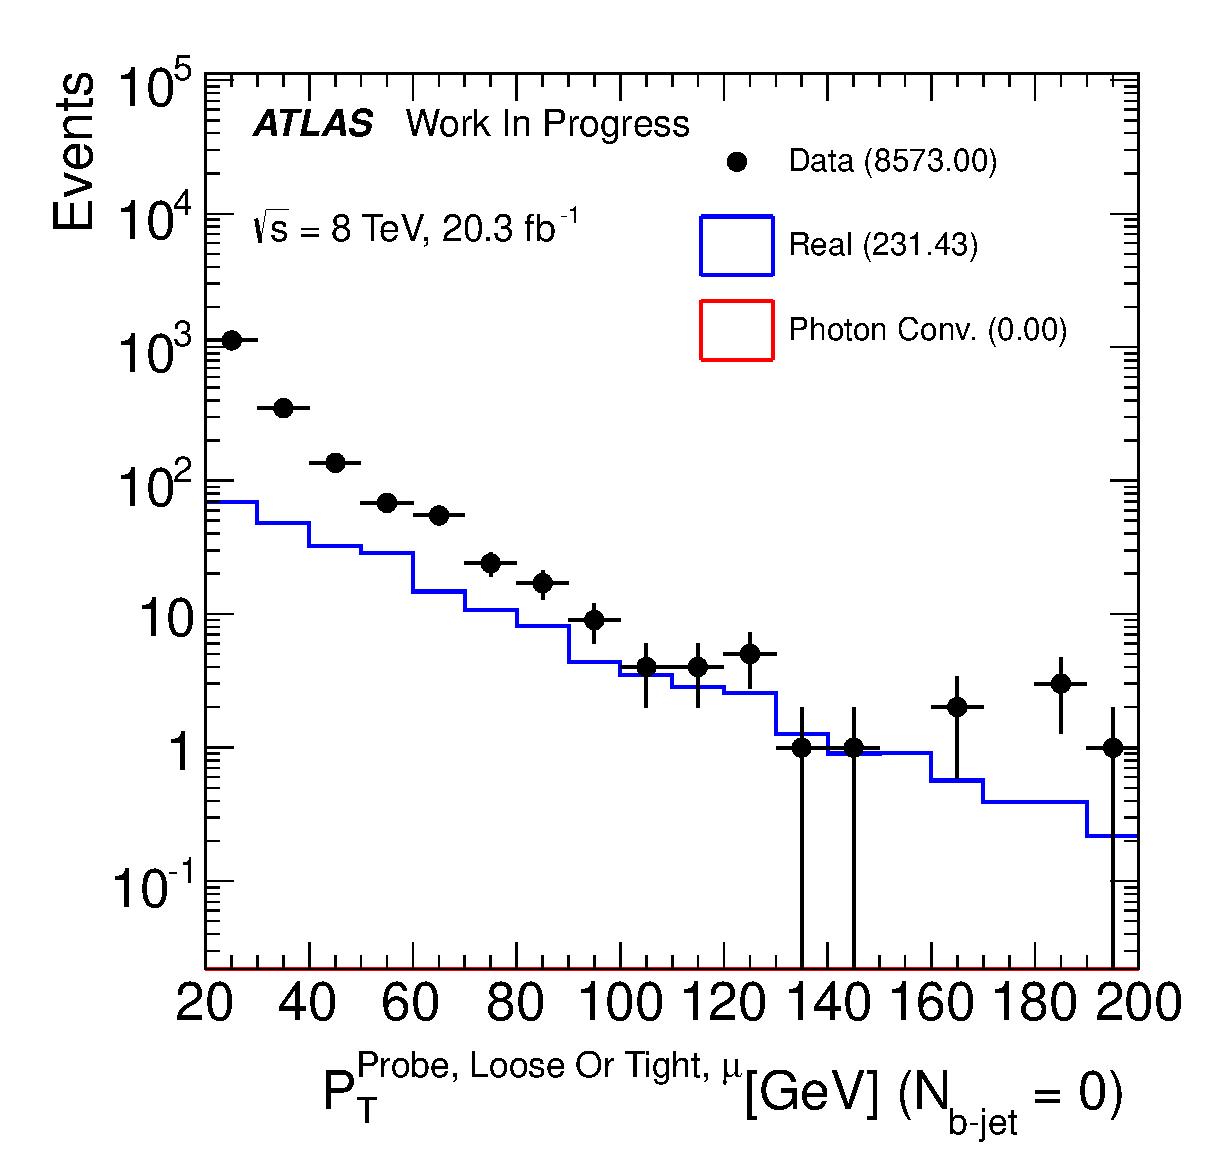
\includegraphics[width=0.45\columnwidth]{figures/fakes_bkg/CRs/SameSignMuonMuon/NoStack/ProbeLooseORTightMuonPtBJetEq0.eps}
%}
\centering
\subfigure{
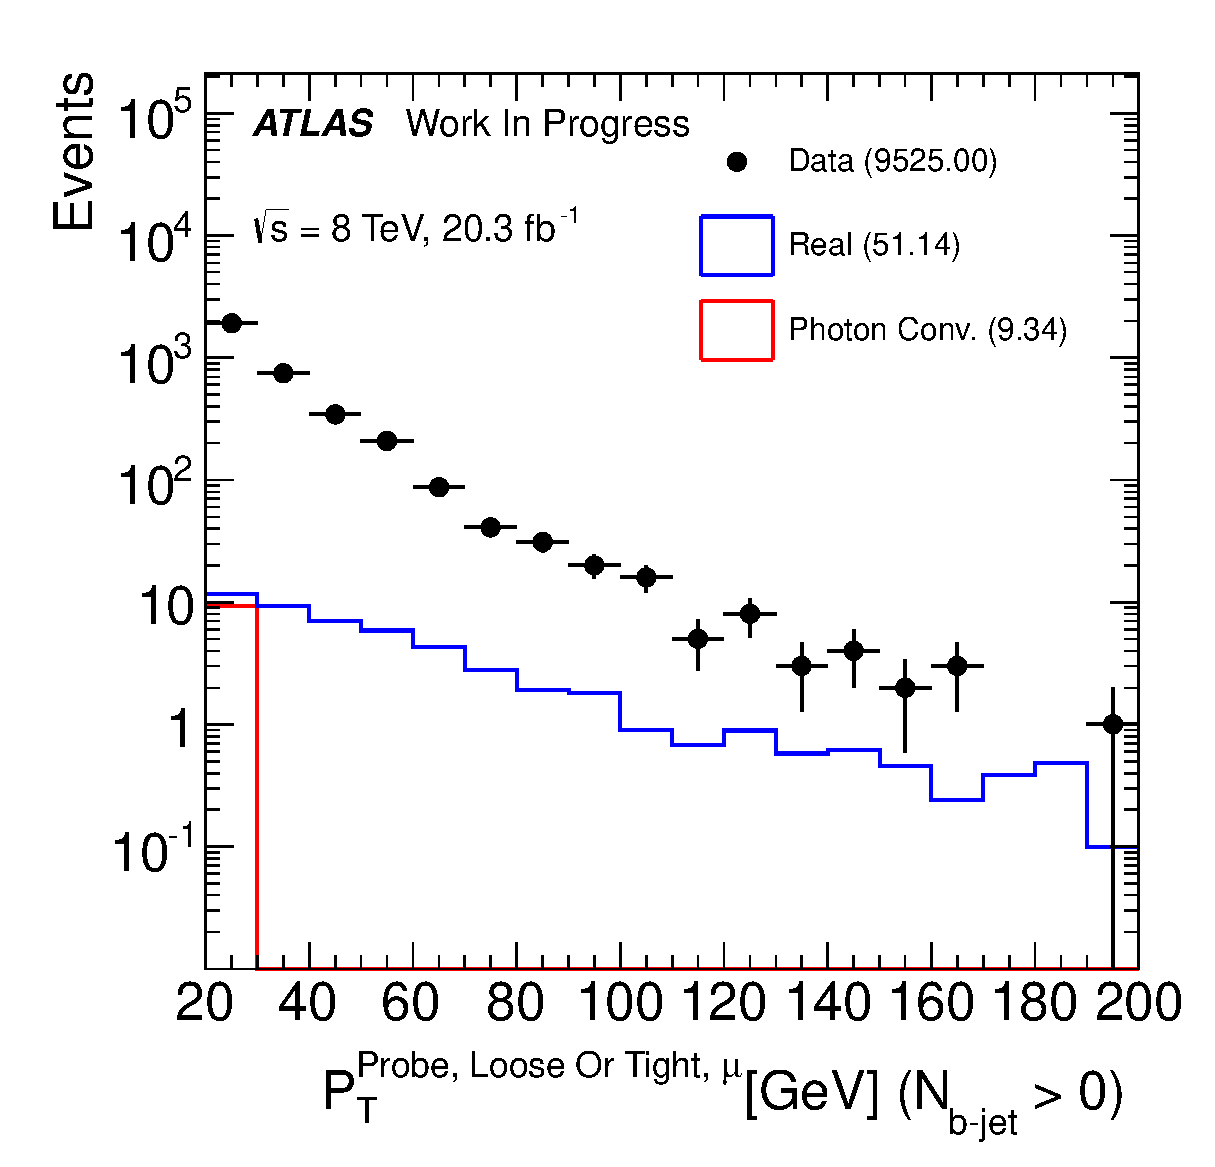
\includegraphics[width=0.45\columnwidth]{figures/fakes_bkg/CRs/SameSignMuonMuon/NoStack/ProbeLooseORTightMuonPtBJetGt0.eps}
}
\vspace{-10mm}\caption{Transverse momentum distributions \pt\ of tight probe muons (top) and loose OR tight probe muons (bottom) passing signal selection criteria in the control Same-Sign $\mu-\mu$ control region without any additional requirement on $b$-jets in the event (left) and at least one $b$-jet (right). 
The amount observed in data (black points) corresponds to $n$ (bottom) and $n_{\textrm{Tight}}$ (top) in Eq.~\ref{eq:fakerate}. 
Meanwhile, the contribution determined in MC to come from real leptons (blue line) and from photon conversion (red line) are shown 
separately; they are not stacked. The real lepton contribution corresponds to 
$n_{\textrm{Tight}}^{\textrm{Real}}$ (top) and $n^{\textrm{Real}}$ (bottom) and the photon conversion 
contribution corresponds to $n_{\textrm{Tight}}^{\textrm{PC}}$ (top) and $n^{\textrm{PC}}$ (bottom) in Eq.~\ref{eq:fakerate}. The photon conversion is 
observed to be negligible for muons.  }
\label{fig:fakeEff_CRs_muon}
\end{figure}

\begin{figure}[h!]
\centering
\subfigure{
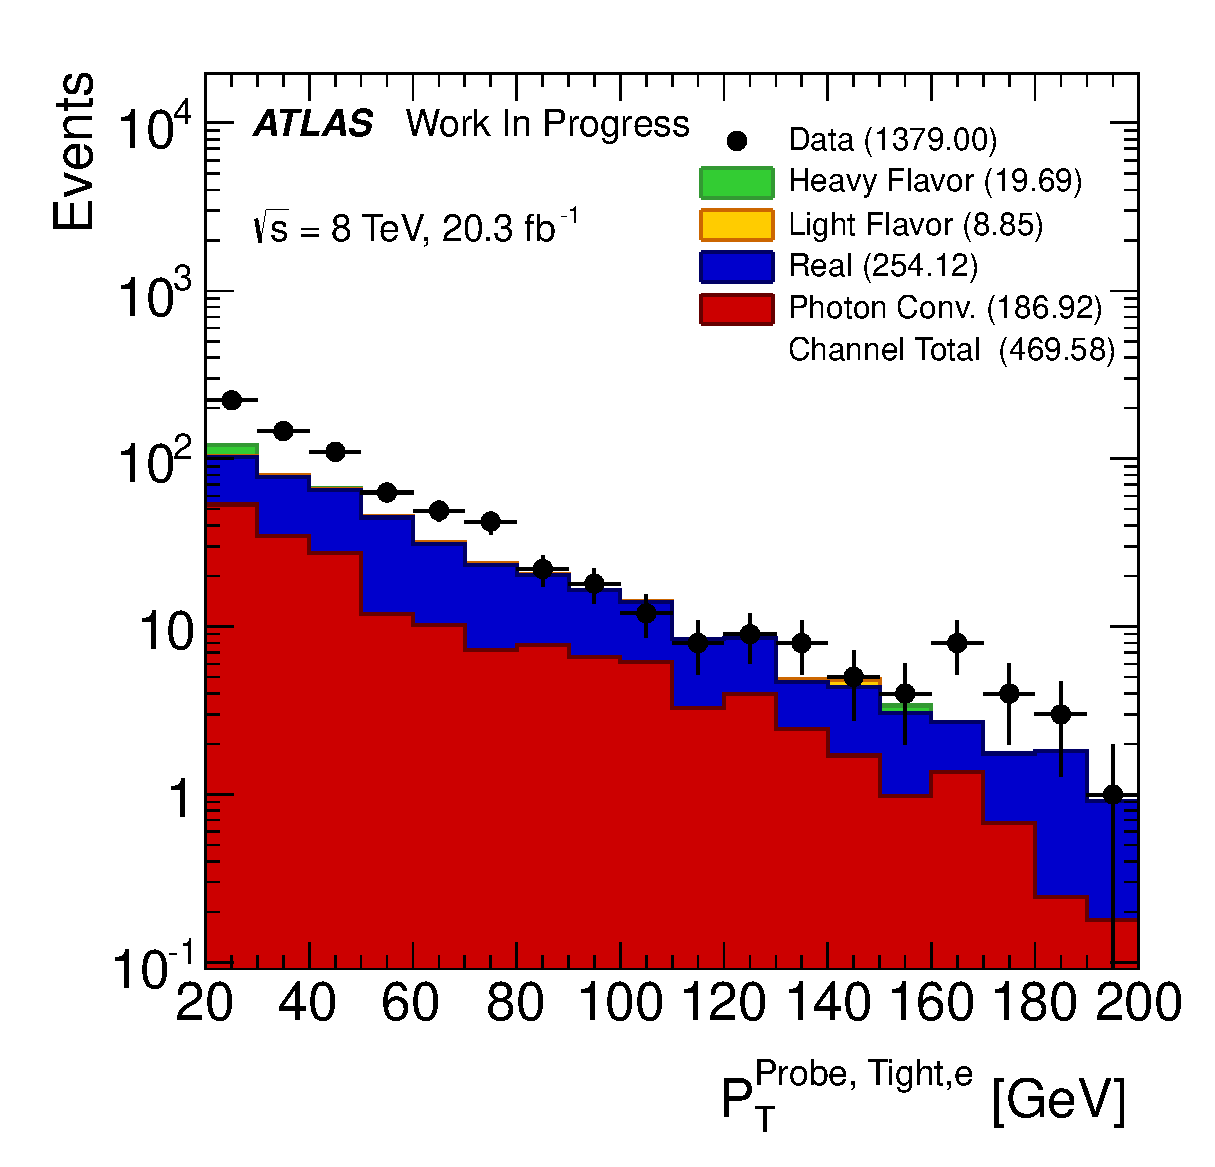
\includegraphics[width=0.45\columnwidth]{figures/fakes_bkg/CRs/SameSignElectronMuon/NoStack/ProbeTightElectronPt.eps}
}
%\centering
%\subfigure{
%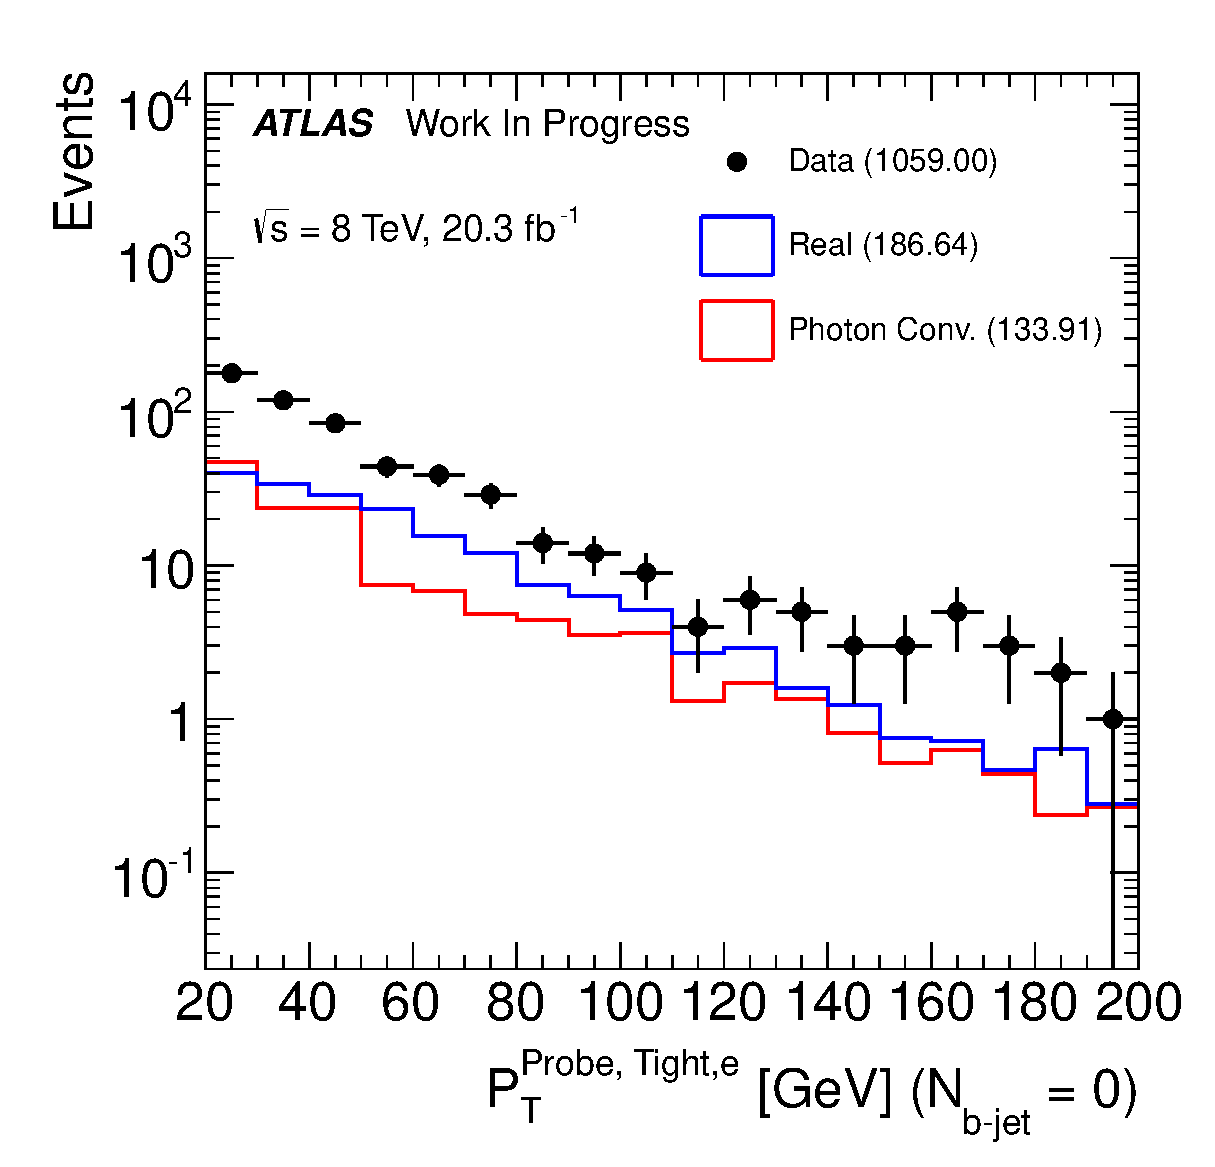
\includegraphics[width=0.3\columnwidth]{figures/fakes_bkg/CRs/SameSignElectronMuon/NoStack/ProbeTightElectronPtBJetEq0.eps}
%}
\centering
\subfigure{
\includegraphics[width=0.45\columnwidth]{figures/fakes_bkg/CRs/SameSignElectronMuon/NoStack/ProbeTightElectronPtBJetGt0.eps}
}
\centering
\subfigure{
\includegraphics[width=0.45\columnwidth]{figures/fakes_bkg/CRs/SameSignElectronMuon/NoStack/ProbeLooseORTightElectronPt.eps}
}
%\centering
%\subfigure{
%\includegraphics[width=0.3\columnwidth]{figures/fakes_bkg/CRs/SameSignElectronMuon/NoStack/ProbeLooseORTightElectronPtBJetEq0.eps}
%}
\centering
\subfigure{
\includegraphics[width=0.45\columnwidth]{figures/fakes_bkg/CRs/SameSignElectronMuon/NoStack/ProbeLooseORTightElectronPtBJetGt0.eps}
}
%\vspace{-1mm}
\vspace{-10mm}\caption{Transverse momentum distributions \pt\ of tight probe electron (top) and loose or tight probe electrons (bottom) passing signal selection criteria in the Same-Sign $e-\mu$ control region without any additional requirement on $b$-jets in the event (left) and at least one $b$-jet (right).
The amount observed in data (black points) corresponds to $n$ (bottom) and $n_{\textrm{Tight}}$ (top) in Eq.~\ref{eq:fakerate}. 
Meanwhile, the contribution determined in MC to come from real leptons (blue line) and from photon conversion (red line) are shown 
separately; they are not stacked. The real lepton contribution corresponds to 
$n_{\textrm{Tight}}^{\textrm{Real}}$ (top) and $n^{\textrm{Real}}$ (bottom) and the photon conversion 
contribution corresponds to $n_{\textrm{Tight}}^{\textrm{PC}}$ (top) and $n^{\textrm{PC}}$ (bottom) in Eq.~\ref{eq:fakerate}.  }
\label{fig:fakeEff_CRs_electron}
\end{figure}






\begin{figure}[ht!]
\centering
\includegraphics[width=0.45\columnwidth]{figures/fakes_bkg/Efficiencies/ElectronFakeRates.png}
\includegraphics[width=0.45\columnwidth]{figures/fakes_bkg/Efficiencies/MuonFakeRates.png}
%\vspace{-10mm}
\caption{Distributions of the electron (left) and muon (right) fake rates as a function of \pt\ extracted in the control regions for three different selections: without any additional requirement on $b$-jets in the event and at least one $b$-jet.}
\label{fig:fakeEff}
\end{figure}




%\tabcolsep=0.1cm
%\begin{table}
%\centering
%\resizebox{0.8\textwidth}{!}{
%\begin{tabular}{l|c|c|c|c|c|c|c} 
%\hline
%\multicolumn{4}{c}{Electrons} &\multicolumn{4}{c}{Muons}\\ \hline
%\pt\ region & Fake eff. & $\sigma_{\mathrm{stat}}$ & $\sigma_{\mathrm{syst}}$ &\pt\ region & Fake eff. & $\sigma_{\mathrm{stat}}$ & $\sigma_{\mathrm{syst}}$ \\\hline
%$\pt \in [10, 15]$ \GeV\ & $0.$ & $0.$ & $0.$ 
%& $\pt \in [10, 15]$ \GeV\ & $0.$ & $0.$ & $0.$ \\
%$\pt \in [15, 30]$ \GeV\ & $0.$ & $0.$ & $0.$
%& $\pt \in [15, 20]$ \GeV\ & $0.$ & $0.$ & $0.$ \\
%$\pt\in [30, 50]$ \GeV\ & $0.$ & $0.$ & $0.$
%& $\pt\in [20, 40]$ \GeV\ & $0.$ & $0.$ & $0.$ \\
%$\pt > 50$ \GeV\ & $0.$ & $0.$ & $0.$
%& $\pt > 40$ \GeV\ & $0.$ & $0.$ & $0.$ \\
%\hline
%\end{tabular}  }
%\caption{Measured fake efficiencies for electrons and muons including statistical and systematic absolute uncertainties.} 
%\label{table:fakeEff_All}
%\end{table} 

\begin{table}[h]
\centering
\begin{tabular}{|l||c|c|c|c||c|c|c|c|}
\hline
 & $\zeta$ & $\sigma_{stat}$ & $\sigma_{sys}^{uncorr}$ & $\sigma_{sys}^{corr}$\\ 
\hline\hline
&\multicolumn{4}{c||}{$N_{b-jet} > 0$}\\ \hline
$p_{T}\in[20,30]$ GeV &  $0.0549$ &  $0.0136$ &  $0.0084$ &  $0.0032$\\ 
$p_{T}\in[30,50]$ GeV &  $0.0645$ &  $0.0272$ &  $0.0203$ &  $0.0161$\\ 
$p_{T} > 50$ GeV &  $0.0816$ &  $0.0723$ &  $0.0764$ &  $0.1088$\\ 
\hline\hline &\multicolumn{4}{c||}{$N_{b-jet} \geq 0$}\\ \hline
$p_{T}\in[20,30]$ GeV &  $0.0995$ &  $0.0141$ &  $0.0270$ &  $0.0099$\\ 
$p_{T}\in[30,50]$ GeV &  $0.1192$ &  $0.0208$ &  $0.0324$ &  $0.0232$\\ 
$p_{T} > 50$ GeV &  $0.1428$ &  $0.0374$ &  $0.0428$ &  $0.0674$\\ 
\hline
\end{tabular}

\caption{Measured fake efficiencies for electrons measured in three regions: with no additional requirements on the presence of $b$-jets and with at least one $b$-jet in a event. Statistical and systematic absolute uncertainties are also shown.} 
\label{table:fakeEff_El}
\end{table} 


\begin{table}[h]
\centering
\begin{tabular}{|l||c|c|c|c||c|c|c|c|}
\hline
 & $\zeta$ & $\sigma_{stat}$ & $\sigma_{sys}^{uncorr}$ & $\sigma_{sys}^{corr}$\\ 
\hline\hline
&\multicolumn{4}{c||}{$N_{b-jet} > 0$}\\ \hline
$p_{T}\in[20,30]$ GeV &  $0.0208$ &  $0.0037$ &  $0.0067$ &  $0.0009$\\ 
$p_{T}\in[30,40]$ GeV &  $0.0207$ &  $0.0066$ &  $0.0113$ &  $0.0020$\\ 
$p_{T} > 40$ GeV &  $0.0492$ &  $0.0109$ &  $0.0259$ &  $0.0068$\\ 
\hline\hline &\multicolumn{4}{c||}{$N_{b-jet} \geq 0$}\\ \hline
$p_{T}\in[20,30]$ GeV &  $0.0378$ &  $0.0046$ &  $0.0140$ &  $0.0040$\\ 
$p_{T}\in[30,40]$ GeV &  $0.0360$ &  $0.0091$ &  $0.0096$ &  $0.0089$\\ 
$p_{T} > 40$ GeV &  $0.0967$ &  $0.0166$ &  $0.0252$ &  $0.0244$\\ 
\hline
\end{tabular}

\caption{Measured fake efficiencies for muons measured in three regions: with no additional requirements on the presence of $b$-jets and with at least one $b$-jet in the event.  Statistical and systematic absolute uncertainties are also shown.} 
\label{table:fakeEff_Mu}
\end{table} 


\clearpage

\subsubsection{Study of the fake lepton composition}
\label{sec:fakecomposition}

The use of the generalized matrix method to determine the 
relies on the assumption that the 
fake rates derived in the di-lepton control regions may be extrapolated to the three lepton signal regions.  
The fake rate depends primarily on the source of the fake leptons, thus
one can check the validity of this assumption by looking at the composition of the
different fake lepton sources in the dilepton control regions and comparing 
them to the
composition in the three lepton signal regions. 

The fake composition is investigated by classifying the MC events as a function of the origin of the fake leptons found in each event.  The MCTruthClassifier tool~\cite{MCtruthclassifier:twiki} is used
to identify the fake laptops origin as follows:

\begin{itemize}
\item Real - Prompt leptons
		\begin{itemize}
		\item \emph{IsoElectron} 
		\item \emph{IsoMuon}
		\item In $Z\gamma$ events classified as either \emph{UnknownElectron} or \emph{UnknownMuon} and parent of lepton is $\gamma$.
		\item In $Z\rightarrow\tau\tau$ events classified as either \emph{NonIsoElectron} or \emph{NonIsoMuon} and lepton has $\tau$ as parent.
		\end{itemize}
\item Heavy Flavor (HF) - Leptons from heavy flavor jets or heavy hadron decays
		\begin{itemize}
		\item \emph{NonIsoElectron} 
		\item \emph{NonIsoMuon}
		\end{itemize}
\item Light Flavor (LF) -  Leptons from light flavor jets
		\begin{itemize}
		\item \emph{Hadron} 
		\item \emph{Others}
		\item In $ZWW$ and $ZZZ$ events classified as either \emph{UnknownElectron} or \emph{UnknownMuon} and parent of lepton is either an up quark, down quark, or a gluon.
		\end{itemize}
\item Photon Conversion (PC)  - Leptons due to radiation
		\begin{itemize}
		\item \emph{BkgElectron} 
		\item \emph{BkgMuon}
		\end{itemize}

\end{itemize}

The composition is shown for electrons in the dilepton control 
regions in Table~\ref{table:CompositionElectronCR} and in the event pre-selection and in region close to the signal regions in Table~\ref{table:CompositionElectronSR}.
First, one can see that the PC contribution is roughly half of the fake contribution
estimate using MC
in the control regions and in the region close to the signal regions. Since this is being estimated
using MC close to the signal regions, 
this component is subtracted out in order to remove any double counting
in the final estimate. Then, after subtraction,
if one compares the composition in the control regions
to the composition in the region close to the signal regions only for electrons, 
in particular after tight selection, one can see that 
the composition is similar for both, 
with about 50 to 75 \% coming from HF and the rest from LF.

For the muons, one can see the composition in the dilepton control regions in 
Table~\ref{table:CompositionMuonCR} and in the event pre-selection
and region close to the signal regions in Table~\ref{table:CompositionMuonSR}. For the muons the PC
component is negligible, as expected, and there is no need for subtraction.
In this case, the composition is dominated by HF, contributing about 90\% with the
rest coming from LF.  This is true in the region close to the signal regions and in the control regions.

The differences observed in the composition between the inclusive $b-jet$ and $b-jet$ 
tagged dilepton control regions is observed to be of a similar size
to the difference in the composition for the region close to the signal regions for both the electron 
and muon cases.
Thus, comparing the rates derived in the control regions using the two different
$b-jet$ criteria should take into account any differences in the composition due
to extrapolation. This is the motivation for choosing the difference in these two 
control regions as an additional systematic on the fake rates.

Using this study of the composition, we conclude that the composition appears to be
consistent between the control regions and the region close to the signal regions.  We have chosen 
a comparison of two different dilepton control regions to be used a systematic
which should take into account any remaining differences in the composition.

It should be said that in the dilepton control regions, 
the MC estimate strongly underestimates the amount observed
in data, presumably because of additional sources of fakes 
not modeled in our MC, such as from QCD. 
The difference in the estimates can be clearly seen in Figures~\ref{fig:fakeEff_CRs_muon_stacked}
and \ref{fig:fakeEff_CRs_electron_stacked} which show the stacked MC estimate from real, photon conversion,
heavy flavor and light flavor sources compared to data.
Thus, the composition estimates shown are only reliable 
if these additional sources would have a similar composition to the ones observed
in this study that we are able to model. This effectively 
puts a large uncertainty on the composition estimates observed in this study. Also,
because the additinonal sources are most likely dominated by QCD, the PC 
contribution to these sources should be small. Thus, the PC component before subtraction
is likely overstated as shown in 
Tables~\ref{table:CompositionElectronCR} 
and \ref{table:CompositionElectronSR}.
As discussed earlier, we subtract the PC
component from the data when obtaining the fake rate. This procedure then assumes
explicitly that all of the photon conversion contribution is modeled in MC and is 
small.


\begin{figure}[h!]
\centering
\subfigure{
\includegraphics[width=0.45\columnwidth]{figures/fakes_bkg/CRs/SameSignMuonMuon/Stacked/ProbeTightMuonPt.eps}
}
%\centering
%\subfigure{
%\includegraphics[width=0.3\columnwidth]{figures/fakes_bkg/CRs/SameSignMuonMuon/Stacked/ProbeTightMuonPtBJetEq0.eps}
%}
\centering
\subfigure{
\includegraphics[width=0.45\columnwidth]{figures/fakes_bkg/CRs/SameSignMuonMuon/Stacked/ProbeTightMuonPtBJetGt0.eps}
}
%\vspace{-1mm}
\centering
\subfigure{
\includegraphics[width=0.45\columnwidth]{figures/fakes_bkg/CRs/SameSignMuonMuon/Stacked/ProbeLooseORTightMuonPt.eps}
}
%\centering
%\subfigure{
%\includegraphics[width=0.45\columnwidth]{figures/fakes_bkg/CRs/SameSignMuonMuon/Stacked/ProbeLooseORTightMuonPtBJetEq0.eps}
%}
\centering
\subfigure{
\includegraphics[width=0.45\columnwidth]{figures/fakes_bkg/CRs/SameSignMuonMuon/Stacked/ProbeLooseORTightMuonPtBJetGt0.eps}
}
\vspace{-10mm}\caption{Transverse momentum distributions \pt\ of tight probe muons (top) and loose OR tight probe muons (bottom) passing signal selection criteria in the control Same-Sign $\mu-\mu$ control region without any additional requirement on $b$-jets in the event (left) and at least one $b$-jet (right). 
The amount observed in data (black points) corresponds to $n$ (bottom) and $n_{\textrm{Tight}}$ (top) in Eq.~\ref{eq:fakerate}. 
Meanwhile, the contribution determined in MC to come from real leptons (blue), photon conversion (red), heavy flavor (green) and light
flavor (orange) are shown stacked on top of each other. 
The difference between the data and MC does not effect the data-driven
fake estimate but may have an impact on the composition estiamte.
}
\label{fig:fakeEff_CRs_muon_stacked}
\end{figure}

\begin{figure}[h!]
\centering
\subfigure{
\includegraphics[width=0.45\columnwidth]{figures/fakes_bkg/CRs/SameSignElectronMuon/Stacked/ProbeTightElectronPt.eps}
}
%\centering
%\subfigure{
%\includegraphics[width=0.3\columnwidth]{figures/fakes_bkg/CRs/SameSignElectronMuon/Stacked/ProbeTightElectronPtBJetEq0.eps}
%}
\centering
\subfigure{
\includegraphics[width=0.45\columnwidth]{figures/fakes_bkg/CRs/SameSignElectronMuon/Stacked/ProbeTightElectronPtBJetGt0.eps}
}
\centering
\subfigure{
\includegraphics[width=0.45\columnwidth]{figures/fakes_bkg/CRs/SameSignElectronMuon/Stacked/ProbeLooseORTightElectronPt.eps}
}
%\centering
%\subfigure{
%\includegraphics[width=0.3\columnwidth]{figures/fakes_bkg/CRs/SameSignElectronMuon/Stacked/ProbeLooseORTightElectronPtBJetEq0.eps}
%}
\centering
\subfigure{
\includegraphics[width=0.45\columnwidth]{figures/fakes_bkg/CRs/SameSignElectronMuon/Stacked/ProbeLooseORTightElectronPtBJetGt0.eps}
}
%\vspace{-1mm}
\vspace{-10mm}\caption{Transverse momentum distributions \pt\ of tight probe electron (top) and loose or tight probe electrons (bottom) passing signal selection criteria in the Same-Sign $e-\mu$ control region without any additional requirement on $b$-jets in the event (left) and at least one $b$-jet (right).
The amount observed in data (black points) corresponds to $n$ (bottom) and $n_{\textrm{Tight}}$ (top) in Eq.~\ref{eq:fakerate}. 
Meanwhile, the contribution determined in MC to come from real leptons (blue), photon conversion (red), heavy flavor (green) and light
flavor (orange) are shown stacked on top of each other.
The difference between the data and MC does not effect the data-driven
fake estimate but may have an impact on the composition estiamte.
}
\label{fig:fakeEff_CRs_electron_stacked}
\end{figure}

%%%%%%%%%%%scaled

%\begin{figure}[h!]
%\centering
%\subfigure{
%\includegraphics[width=0.45\columnwidth]{figures/fakes_bkg/CRs/SameSignMuonMuon/Scaled/coarse/ProbeTightMuonPtFakeRate_histratio.png}
%}
%\centering
%\subfigure{
%\includegraphics[width=0.45\columnwidth]{figures/fakes_bkg/CRs/SameSignMuonMuon/Scaled/coarse/ProbeTightMuonPtBJetGt0FakeRate_histratio.png}
%}
%\centering
%\subfigure{
%\includegraphics[width=0.45\columnwidth]{figures/fakes_bkg/CRs/SameSignMuonMuon/Scaled/coarse/ProbeLooseORTightMuonPtFakeRate_histratio.png}
%}
%\centering
%\subfigure{
%\includegraphics[width=0.45\columnwidth]{figures/fakes_bkg/CRs/SameSignMuonMuon/Scaled/coarse/ProbeLooseORTightMuonPtBJetGt0FakeRate_histratio.png}
%}
%\vspace{-10mm}\caption{Scaled....Transverse momentum distributions \pt\ of tight probe muons (top) and loose OR tight probe muons (bottom) passing signal selection criteria in the control Same-Sign $\mu-\mu$ control region without any additional requirement on $b$-jets in the event (left) and at least one $b$-jet (right). 
%The amount observed in data (black points) corresponds to $n$ (bottom) and $n_{\textrm{Tight}}$ (top) in Eq.~\ref{eq:fakerate}. 
%Meanwhile, the contribution determined in MC to come from real leptons (blue), photon conversion (red), heavy flavor (green) and light
%flavor (orange) are shown stacked on top of each other. 
%The difference between the data and MC does not effect the data-driven
%fake estimate but may have an impact on the composition estiamte.
%}
%\label{fig:fakeEff_CRs_muon_stacked_scaled}
%\end{figure}

%\begin{figure}[h!]
%\centering
%\subfigure{
%\includegraphics[width=0.45\columnwidth]{figures/fakes_bkg/CRs/SameSignElectronMuon/Scaled/coarse/ProbeTightElectronPtFakeRate_histratio.png}
%}
%\centering
%\subfigure{
%\includegraphics[width=0.45\columnwidth]{figures/fakes_bkg/CRs/SameSignElectronMuon/Scaled/coarse/ProbeTightElectronPtBJetGt0FakeRate_histratio.png}
%}
%\centering
%\subfigure{
%\includegraphics[width=0.45\columnwidth]{figures/fakes_bkg/CRs/SameSignElectronMuon/Scaled/coarse/ProbeLooseORTightElectronPtFakeRate_histratio.png}
%}
%\centering
%\subfigure{
%\includegraphics[width=0.45\columnwidth]{figures/fakes_bkg/CRs/SameSignElectronMuon/Scaled/coarse/ProbeLooseORTightElectronPtBJetGt0FakeRate_histratio.png}
%}
%\vspace{-10mm}\caption{Scaled...Transverse momentum distributions \pt\ of tight probe electron (top) and loose or tight probe electrons (bottom) passing signal selection criteria in the Same-Sign $e-\mu$ control region without any additional requirement on $b$-jets in the event (left) and at least one $b$-jet (right).
%The amount observed in data (black points) corresponds to $n$ (bottom) and $n_{\textrm{Tight}}$ (top) in Eq.~\ref{eq:fakerate}. 
%Meanwhile, the contribution determined in MC to come from real leptons (blue), photon conversion (red), heavy flavor (green) and light
%flavor (orange) are shown stacked on top of each other.
%The difference between the data and MC does not effect the data-driven
%fake estimate but may have an impact on the composition estiamte.
%}
%\label{fig:fakeEff_CRs_electron_stacked_scaled}
%\end{figure}


\begin{table}[ht!]
\centering
\begin{tabular}{|lc|ccc|}
    \hline
    \multicolumn{5}{|c|}{\bf{Control regions}}   \\ \hline \hline
    PC subtracted &$N_{b-jet}$  &{HF} &{PC} &{LF} \\ \hline
    yes &--- &$57\pm 4$\%  &$0$\% &$43\pm 6$\% \\
    yes &$N_{b-jet}>0$  &$75\pm 5$\% &$0$\% &$25\pm 3$\% \\ \hline
    no &--- &$22\pm 3$\% &$61\pm 13$\% &$17\pm 3$\% \\
    no &$N_{b-jet}>0$  &$43\pm 3$\% &$42\pm 6$\% &$15\pm 2$\% \\ 
    \hline
	
\end{tabular}




\caption{
Composition of fake electrons taken from  MC events in the same-sign electron-muon dilepton control regions
used to extract electron fake rates. The composition is split as either Heavy Flavor (HF), Photon
Conversion (PC), and Light Flavor (LF) are shown. In the ``PC subtracted'' case, the PC component
has been explicitly removed.  This corresponds to the scenario ultimately used in the
fake rate estimation.
}
\label{table:CompositionElectronCR}
\end{table}

\begin{table}[ht!]
\centering
    \begin{tabular}{|l||cc|}
    \hline 
    \multicolumn{3}{|c|}{\bf{Pre-selection and signal regions}}   \\ 
    & Heavy Flavor & Light Flavor \\
    \hline \hline
    \hline

    Pre-selection &$53.7 \pm 9.4$\% & $46.3\pm 10.0$\% \\
    0 SFOS &$80.2 \pm 19.9$\% & $19.8\pm 11.8$\% \\
    1 SFOS &$52.4 \pm 12.5$\% & $47.6\pm 11.9$\% \\
    2 SFOS &$47.7 \pm 16.1$\% & $52.3\pm 23.3$\% \\
    \hline


  \end{tabular}
  








\caption{
Composition of fake electrons taken from  MC events in the event pre-selection and regions close to the signal regions used in the analysis. 
The composition is split as either Heavy Flavor (HF) or Light Flavor (LF). 
}
\label{table:CompositionElectronSR}
\end{table}


\begin{table}[ht!]
\centering
    \begin{tabular}{|lc|ccc|}
    \hline
    \multicolumn{5}{|c|}{\bf{Control regions}}   \\ \hline \hline
    PC subtracted &$N_{b-jet}$  &{HF} &{PC} &{LF} \\ \hline
    yes &--- &$89\pm 4$\% &$0$\% &$11\pm 1$\% \\
    yes &$N_{b-jet}>0$  &$95\pm 3$\% &$0$\% &$4\pm 1$\%\\ \hline
    no &--- &$89\pm 4$\% &$0$\% &$11\pm 1$\% \\
    no &$N_{b-jet}>0$  &$95\pm 3$\% &$0$\% &$4\pm 1$\%\\ 
    %\color{yellow!70!black}\met\ $>10$GeV &\color{yellow!70!black}$N_{b-jet}>1$  &\color{yellow!70!black}91\% &\color{yellow!70!black}0\% &\color{yellow!70!black}9\% \\ 
    \hline
  \end{tabular}
  

\caption{
Composition of fake muons taken from  MC events in the event pre-selection and regions close to the signal regions used in the analysis. 
The composition is split as either Heavy Flavor (HF), Photon
Conversion (PC), and Light Flavor (LF) are shown. The photon conversion component
is measured to be negligible. No PC subtraction is performed.
}
\label{table:CompositionMuonCR}
\end{table}

\begin{table}[ht!]
\centering
    \begin{tabular}{|l||cc|}
    \hline 
    \multicolumn{3}{|c|}{\bf{Pre-selection and signal regions}}   \\ 
    & Heavy Flavor & Light Flavor \\
    \hline \hline
    \hline

    Pre-selection &$78.9 \pm 10.0$\% & $21.1\pm 4.6$\% \\
    0 SFOS &$96.7 \pm 21.0$\% & $3.3\pm 3.7$\% \\
    1 SFOS &$77.4 \pm 14.1$\% & $22.6\pm 7.2$\% \\
    2 SFOS &$77.3 \pm 15.9$\% & $22.8\pm 7.1$\% \\
    \hline


  \end{tabular}
  








\caption{
Composition of fake muons taken from  MC events in the same-sign muon-muon dilepton control regions
used to extract the muon fake rates. The composition is split into either Heavy Flavor (HF) or Light Flavor (LF). 
}
\label{table:CompositionMuonSR}
\end{table}

\clearpage
\subsubsection{Fake lepton background validation}

A Monte Carlo closure test of the generalized matrix method is performed. The fake rates are computed from MC samples in the dilepton control regions defined in section~\ref{sec:fakecomposition}, and the method is then applied on the most important MC samples contributing to the event pre-selection: $Z$+jets and $t\bar{t}$. The event pre-selection is used for this test, because the statistics available for the MC samples containing fake leptons in the signal region is too small to be able to draw any conclusion. Figure~\ref{fig:MCFakeRatesClosure}, show the MC fake rates obtained from the CR, while figure~\ref{fig:MCClosureCheckMatrixMethod} show the MC agreement with the MC events reweighted using the generalized matrix method in the event pre-selection region, for the third-leading lepton $\pt$ and the $\met$ distribution. As it can be seen the shape agreement and the overall normalization are pretty good, showing that the matrix method is performing well.

\begin{figure}[ht!]
\centering
\includegraphics[width=0.42\columnwidth]{figures/ClosureCheck_MatrixMethod/ElFakeRates_MC_topZjets_new.pdf}
\includegraphics[width=0.42\columnwidth]{figures/ClosureCheck_MatrixMethod/MuFakeRates_MC_topZjets_new.pdf}
\caption{Distribution of the fake rates obtained from MC samples in the dilepton control regions. The errors shown here are statistical only. These rates are used to performed a MC closure check of the global matrix method.}
\label{fig:MCFakeRatesClosure}
\end{figure}

\begin{figure}[ht!]
\centering
\includegraphics[width=0.42\columnwidth]{figures/ClosureCheck_MatrixMethod/PtThirdLepSignal_TTT_total_new.pdf}
\includegraphics[width=0.42\columnwidth]{figures/ClosureCheck_MatrixMethod/VR_PMET_lepTTT_total_new.pdf}
\caption{Distributions of the third leading lepton $\pt$ and $\met$ in the event pre-selection region, for $Z$+jets and $t\bar{t}$, compared to events from these samples reweigthed using the global matrix method and the rates shown in Figure~\ref{fig:MCFakeRatesClosure}. Good agreement is observed}
\label{fig:MCClosureCheckMatrixMethod}
\end{figure}




The ability of the generalized matrix method just described to model accurately
the fake lepton background is tested in a control region designed to be enhanced
in the fake lepton background while mainitaining orthogonality with the signal
regions described in Section~\ref{sec:signal_regions}. The control region 
starts by using the event pre-selection region described in Section~\ref{sec:preselection}. To reduce contamination in the 
control region from the $WZ$ process, it is required that none
of the three leptons selected form a Same-Flavor Opposite-Sign lepton pair.
Finally, to ensure orthogonality with the signal regions which require that no
$b$-tagged jets are present in the event, this control region requires
the presence of at least one $b$-tagged jet in the event. 

This control region
is clearly dominated by the data-driven fake lepton background as can
be seen in Fig.~\ref{fig:FakeCR} and in Table~\ref{tab:FakeCR}. 
Furthermore, Table~\ref{tab:FakeCR} shows good agreement between data
and the fake background modeling on the total event yield, which is within 
the statistical uncertainties.  One can even see from
Fig.~\ref{fig:FakeCR} that the shape description does a reasonable job,
although the statistical uncertainty is a bit too large to draw strong conclusions.
One can also see that the systematic uncertainty easily covers most
of the differences that are observed. Thus, we conclude that the fake background
description is working and may be used in our signal regions.  Especially since
the fake background is most important in the 0 SFOS region (described in more
detail in Section~\ref{sec:signal_regions}) which differs primarily from this
control region only by the $b$-veto requirement.




\begin{figure}[ht!]
\centering
\includegraphics[width=0.3\columnwidth]{figures/Fake_CR/LeadingLeptonPt_histratio.eps}
\includegraphics[width=0.3\columnwidth]{figures/Fake_CR/SubleadingLeptonPt_histratio.eps}
\includegraphics[width=0.3\columnwidth]{figures/Fake_CR/MinimumLeptonPt_histratio.eps}
\includegraphics[width=0.3\columnwidth]{figures/Fake_CR/MET_Et_histratio.eps}
\includegraphics[width=0.3\columnwidth]{figures/Fake_CR/NBTaggedJets_histratio.eps}
\includegraphics[width=0.3\columnwidth]{figures/Fake_CR/NJets_histratio.eps}
\includegraphics[width=0.3\columnwidth]{figures/Fake_CR/NMuons_histratio.eps}
\caption{Distributions in a control region designed to study the data-driven fake lepton background estimate.  The selection used is as follows: Event pre-selection + 0 SFOS + at least 1 $b$-jet.  Good agreement is observed}
\label{fig:FakeCR}
\end{figure}

\begin{table}[ht!]
\centering
\begin{tabular}{|c||c|c|c|c|}
\hline
 & Event Yield\\ 
\hline\hline
$WZ$ &  $0.338 \pm 0.021$\\ 
$ZZ$ &  $0.0747 \pm 0.0064$\\ 
$Z\gamma$ &  $0.0058 \pm 0.0058$\\ 
$ZWW+ZZZ$ &  $0.026 \pm 0.005$\\ 
$t\bar{t}+V$ &  $3.228 \pm 0.039$\\ 
Fake (data-driven) &  $10.91 \pm 0.73$\\ 
$WWW$ &  $0.1431 \pm 0.0052$\\ 
\hline
Expected Background &  $14.58 \pm 0.73$\\ 
Expected Signal + Background &  $14.72 \pm 0.73$\\ 
\hline
Observed Data &  $18$\\ 
\hline
\end{tabular}

\caption{Expected and observed yields for the fake lepton control region.}
\label{tab:FakeCR}
\end{table}



